\documentclass[12pt]{article}
\usepackage{url}
\usepackage{listings}
\usepackage{graphicx}
\usepackage{float}
\usepackage{titlesec}
\usepackage{CJK}
\begin{CJK}{UTF8}{gkai}
\title{Linux内核0.01源代码分析}
\author{Chuzy}
\date{2020/05/03}
%以上部分叫做"导言区",下面才开始写正文
\begin{document}
%先插入标题
\maketitle
\tableofcontents
\newpage 

\section{版本概况}
\paragraph{•}
这是第一个正式对外公布的Linux版本,含多线程文件系统、分段和分页内存管理,还不包含软盘驱动程序。
\begin{figure}[htbp]
\centering
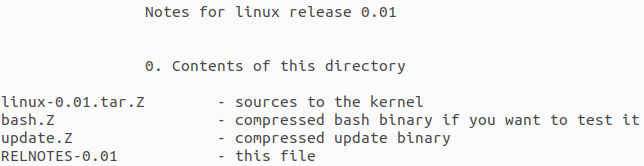
\includegraphics[scale=0.5]{fig/1.png}
\caption{第一个内核版本包}
\label{fig:Content of Linux 0.01}
\end{figure}
\begin{list}{•}{•}
\item 第一个文件夹boot,实现计算机加电自检引导扇区;
\item 第二个文件夹fs ,也就是文件系统file system;
\item 第三个文件夹include,头文件都聚集在这里;
\item 第四个文件夹init,main函数在这里;
\item 第五个文件夹kernel,内核代码文件;
\item 第六个文件夹lib,库文件;
\item 第七个文件夹mm,内存管理;
\item 第八个文件夹tools,只有内核是没有用的,这里包含shell的bin文件
\end{list}
%\subparagraph{123}
\section{Makefile}
\paragraph{•}
相对0.00版本,0.01版本的文件数量大大增加,Makefile也变得更加复杂。我们分成几个小节来分别研究。
\subsection{编译工具链}
\paragraph{•}
在Unbutu 1910版本中,工具链已经发生了比较大的变化。
\begin{list}{•}{•}
\item 现象1: 提示gas gld 不识别,措施:用gcc替代;
\item 现象2: 提示字节对齐需要是2的倍数,措施:利用命令
sed -i 's/align 2/align 4/g' filename
替换align 2 为 align 4(align 3 替换为 align 8);
\item 现象3: -fcombine-regs -mstring-insns选项不识别, 措施:此两个选项已经过时,直接去掉即可;
\item 现象4: warning 特别多, 措施:将-Wall 替换为 -w;
\item 现象5: main.c 中\_syscall0重复定义, main.c static inline \_syscall0(int, fork) 去掉static即可;
\item 现象6: 提示内嵌汇编不符合语法限制, 'asm' operand has impossible constraints. 措施:类似的问题在后面编译中出现好多,C内嵌汇编的格式asm(汇编语句:输入寄存器:输出寄存器:可能被修改的寄存器),最新的GCC规定 输入或输出寄存器不能出现在可能被修改的寄存器中,目前看到网上的方法是把所有类似问题的可能被修改的寄存器全部删掉;
\item 现象7: keyboard.s,`\%al' not allowed with `xorl',将xorl替换为xorb;
\item 现象8: traps.c,'get\_super' 被多次定义,类似错误出现很多,将segment.h string.h mm.h中定义的函数extern inline全部改成static inline的;
\item 现象9 : file\_dev.c: In function 'file\_read', unsupported size for integer register, 需要关闭编译优化来解决,即去掉gcc编译参数中的-O,采用默认值(-O0);
\item 现象10 :链接错误, head.o: In function `startup\_32'...,错误原因为是过去的gcc编译器会把符号前加下划线,现代gcc去除这一规则,此处将.s中引用.c中的及.s提供给.c使用的所有符号前的下划线去掉。
\item 现象11: \_\_stack\_chk\_fail 未定义, 需要在Makefile中的\$(CFLAGS)后面加上-fno-stack-protector,即不需要栈保护

%原文链接:https://blog.csdn.net/lp_19880801/java/article/details/80800651
%现象8: 在 control.c 中清楚定义了 static unsigned char attr = 0x70,而在链接 control.o 时,却爆出 attr未定义。
%措施:用 nm -C control.o 查看其符号,发现attr确实处于未定义状态。故单独编译一个小程序定义静态变量,查看其 .o 文件中,发现静态变量定义正常。故考虑为编译选项差异导致,最终发现因为 -O 编译优化选项导致,目前处理方式是去掉该选项。
%现象9: build.c:(.text+0xde): undefined reference to `MAJOR'
%措施: 通过分析编译打印信息,发现编译时没有加入头文件路径 -Iinclude
%现象10: fs/fs.o: In function check_disk_change':(.text+0x1b2f): undefined reference toinvalidate_buffers'
%措施: 查找发现此函数定义在buffer.c 中,且为内联函数, 故尝试将其更改为普通函数, 然后编译通过.
%现象11: 编译 build.c 时报错:/usr/include/i386-linux -gnu/bits/stdio2.h:57:8: error: unknown type name ‘__gnuc_va_list’
%措施: 分析发现时此系列错误均由 -Iinclude 选项导致, 而该选项在想象9中加入, 故考虑去掉该选项, 直接在build.c 中加入 MAJOR 宏定义.
\end{list}

\begin{lstlisting}[breaklines]
AS86	=as -0 -a
CC86	=cc -0
LD86	=ld -0

AS	=gas
LD	=gld
LDFLAGS	=-s -x -M
CC	=gcc
CFLAGS	=-Wall -O -fstrength-reduce -fomit-frame-pointer -fcombine-regs
CPP	=gcc -E -nostdinc -Iinclude
\end{lstlisting}
\begin{lstlisting}
ARCHIVES=kernel/kernel.o mm/mm.o fs/fs.o
LIBS	=lib/lib.a

.c.s:
	$(CC) $(CFLAGS) \
	-nostdinc -Iinclude -S -o $*.s $<
.s.o:
	$(AS) -c -o $*.o $<
.c.o:
	$(CC) $(CFLAGS) \
	-nostdinc -Iinclude -c -o $*.o $<

all:	Image

Image: boot/boot tools/system tools/build
	tools/build boot/boot tools/system > Image
	sync

tools/build: tools/build.c
	$(CC) $(CFLAGS) \
	-o tools/build tools/build.c
	chmem +65000 tools/build

boot/head.o: boot/head.s

tools/system:	boot/head.o init/main.o \
		$(ARCHIVES) $(LIBS)
	$(LD) $(LDFLAGS) boot/head.o init/main.o \
	$(ARCHIVES) \
	$(LIBS) \
	-o tools/system > System.map

kernel/kernel.o:
	(cd kernel; make)

mm/mm.o:
	(cd mm; make)

fs/fs.o:
	(cd fs; make)

lib/lib.a:
	(cd lib; make)

boot/boot:	boot/boot.s tools/system
	(echo -n "SYSSIZE = (";ls -l tools/system | grep system \
		| cut -c25-31 | tr '\012' ' '; echo "+ 15 ) / 16") > tmp.s
	cat boot/boot.s >> tmp.s
	$(AS86) -o boot/boot.o tmp.s
	rm -f tmp.s
	$(LD86) -s -o boot/boot boot/boot.o

clean:
	rm -f Image System.map tmp_make boot/boot core
	rm -f init/*.o boot/*.o tools/system tools/build
	(cd mm;make clean)
	(cd fs;make clean)
	(cd kernel;make clean)
	(cd lib;make clean)

backup: clean
	(cd .. ; tar cf - linux | compress16 - > backup.Z)
	sync

dep:
	sed '/\#\#\# Dependencies/q' < Makefile > tmp_make
	(for i in init/*.c;do echo -n "init/";$(CPP) -M $$i;done) >> tmp_make
	cp tmp_make Makefile
	(cd fs; make dep)
	(cd kernel; make dep)
	(cd mm; make dep)

### Dependencies:
init/main.o : init/main.c include/unistd.h include/sys/stat.h \
  include/sys/types.h include/sys/times.h include/sys/utsname.h \
  include/utime.h include/time.h include/linux/tty.h include/termios.h \
  include/linux/sched.h include/linux/head.h include/linux/fs.h \
  include/linux/mm.h include/asm/system.h include/asm/io.h include/stddef.h \
  include/stdarg.h include/fcntl.h 
\end{lstlisting}

%    #
%    # Makefile for linux.
%    # If you don't have '-mstring-insns' in your gcc (and nobody but me has :-)
%    # remove them from the CFLAGS defines.
%    #
%    #
%    #8086汇编编译器和连接器. -0生成8086目标程序;-a生成与gas和gld部分兼容的代码
%    #
%    AS86 =as -0 -a
%    CC86 =cc -0
%    LD86 =ld -0
%    #
%    #GNU汇编编译器和连接器
%    #
%    AS =gas
%    LD =gld
%    #
%    #GNU连接器gld运行时用到的选项
%    #-s 输出文件中省略所有的符号信息
%    #-x 删除所有的局部符号
%    #-M 在标准输出设备(显示器)上打印连接映象(link map).
%    #连接映象:由连接程序产生的一种内存地址映象,其中列出了程序装入到内存中的位置信息,具体有如下信息:
%    #目标文件及符号信息映射到内存中的位置
%    #公共符号如何放置
%    #连接中包含的所有文件成员及其引用的符号
%    #
%    LDFLAGS =-s -x -M
%    #
%    #gcc是GNU C程序编译器,对于UNIX类的脚本程序而言,
%    #在引用定义的标识符时,需在前面加上$符号并用括号括住标识符
%    #
%    CC =gcc
%    #
%    #GCC的选项.
%    #-Wall 打印所有的警告信息
%    #-O 对代码进行优化
%    #-fstrength-reduce 优化循环语句
%    #
%    CFLAGS =-Wall -O -fstrength-reduce -fomit-frame-pointer -fcombine-regs
%    #
%    #CPP是gcc的预处理程序
%    #-nostdinc -Iinclude 不要搜索标准的头文件目录中的文件,
%    #而是使用-I选项指定的目录或者是在当前的目录里搜索头文件
%    #
%    CPP =gcc -E -nostdinc -Iinclude
%    #
%    # kernel目录,mm目录,fs目录所产生的目标代码文件。
%    # 为了方便引用,在这里将它们用ARCHIVES(归档文件)标识符表示
%    #
%    ARCHIVES=kernel/kernel.o mm/mm.o fs/fs.o
%    #
%    # 由lib/目录中生成的通用库文件
%    #
%    LIBS =lib/lib.a
%    #
%    # make隐式后缀规则
%    # 指示make利用下面的命令将所有的.c文件编译生成.s汇编程序
%    # ':'表示下面是该规则的命令
%    # 规则:指使gcc采用前面CFLAGS所指定的选项以及仅使用include/目录中的头文件,
%    # 在适当的编译后不进行汇编就停止(-S),从而产生与输入的各个C文件对应的汇编语言形式的代码文件。
%    # 默认情况下所产生的汇编程序文件是原C文件名去掉.c而加上.s后缀。
%    # -o表示其后是输出文件的形式。
%    # 其中$*.s(或$@)是自动目标变量,$<代表第一个先决条件,这里即是符合条件*.c的文件。
%    #
%    .c.s:
%    $(CC) $(CFLAGS) \
%    -nostdinc -Iinclude -S -o $*.s $<
%    #
%    # 将所有.s汇编程序文件编译成.o目标文件。下一条是实现该操作的具体命令
%    # 使用gas编译器将汇编程序编译成.o目标文件。-c表示只编译或汇编,但不进行连接操作
%   #
%    .s.o:
%    $(AS) -c -o $*.o $<
%    #
%    # 使用gcc将c语言编译成目标文件但不连接
%    #
%    .c.o:
%    $(CC) $(CFLAGS) \
%    -nostdinc -Iinclude -c -o $*.o $<
%    #
%    # all表示创建Makefile所知的最顶层目标。这里即是image文件
%    #
%    all: Image
%    #
%    # 第一行说明:目标文件(Image文件)是由分号后面的3个元素产生
%    # 下面两行是执行的命令
%    # 第一行表示使用tools目录下的build工具程序将boot,system文件组装成内核映象文件Image
%    # 第二行的sysn同步命令是迫使缓冲块数据立即写盘并更新超级块
%    #
%    Image: boot/boot tools/system tools/build
%    tools/build boot/boot tools/system > Image
%    sync
%    #chmem -- 修改系统内存数据
%    tools/build: tools/build.c
%    $(CC) $(CFLAGS) \
%    -o tools/build tools/build.c
%    chmem +65000 tools/build
%    #
%    # 利用上面的.s.o规则生成head.o文件
%    #
%    boot/head.o: boot/head.s
%    #
%    # 最后的>System.map表示gld需要将连接映象重定向存放在System.map文件中
%    #
%    tools/system: boot/head.o init/main.o \
%    $(ARCHIVES) $(LIBS)
%    $(LD) $(LDFLAGS) boot/head.o init/main.o \
%    $(ARCHIVES) \
%    $(LIBS) \
%    -o tools/system > System.map
%    #
%    # 内核目标模块kernel.o
%    #
%    kernel/kernel.o:
%    (cd kernel; make)
%    #
%    # 内核管理模块mm.o
%    #
%    mm/mm.o:
%    (cd mm; make)
%    #
%    # 文件系统目标模块fs.o
%    #
%    fs/fs.o:
%    (cd fs; make)
%    #
%    # 库函数lib.a
%    #
%    lib/lib.a:
%    (cd lib; make)
%    #
%    # 在boot.s程序开口添加一行有关system文件长度信息
%    # 首先生成含有 "SYSSIZE = 文件实际长度"一行信息的tmp.s文件,然后将boot.s文件添加在其后。
%    # 取得system长度的方法是:
%    # 利用ls命令对system文件进行长列表显示
%    # 用grep命令取得列表上文件字节数字段信息,并定向保存在tmp.s临时文件中
%    # cut命令用于剪切字符串
%    # tr用于去除行尾的回车符
%    # (实际长度 + 15)/16用于获得'节'表示的长度信息,1节=16字节
%    # 用8086汇编和连接器对setup.s文件进行编译生成setup文件
%    # -s表示要取出目标文件中的符号信息
%    #
%    boot/boot: boot/boot.s tools/system
%    (echo -n "SYSSIZE = (";ls -l tools/system | grep system \
%    | cut -c25-31 | tr '\012' ' '; echo "+ 15 ) / 16") > tmp.s
%    cat boot/boot.s >> tmp.s
%    $(AS86) -o boot/boot.o tmp.s
%    rm -f tmp.s
%    $(LD86) -s -o boot/boot boot/boot.o
%    #
%    # 当执行"make clean"时,就会执行以下命令,去除所有编译连接生成的文件
%    # "rm"是文件删除命令,选项-f含义是忽略不存在的文件,并且不显示删除信息
%    # (cd mm;make clean)表示进入mm/目录,执行该目录Makefile文件中的clean规则
%    #
%    clean:
%    rm -f Image System.map tmp_make boot/boot core
%    rm -f init/*.o boot/*.o tools/system tools/build
%    (cd mm;make clean)
%    (cd fs;make clean)
%    (cd kernel;make clean)
%    (cd lib;make clean)
%    #
%    # 该规则首先执行上面的clean规则,然后对linux/目录进行压缩,生成backup.Z压缩文%件。
%    # "cd .."表示退到linux/的上一级(父)目录
%    # "tar cf - linux"表示对linux/目录执行tar归档程序,-cf表示需要创建新的归档文件
%    # "| compress -"表示将tar程序的执行通过管道操作('|')传递给压缩程序compress,并将压缩程序的输
%    #出存成backup.Z文件
%    # sysn同步命令迫使缓冲块数据立即写盘并更新超级块
%    #
%    backup: clean
%    (cd .. ; tar cf - linux | compress16 - > backup.Z)
%    sync
%    #
%    # 该规则用于各文件的依赖关系。创建这些依赖关系是为了给make用来确定是否需要重建一个目标对象
%    # 比如当某个文件头被改动过后,make就通过生成的依赖关系,重新编译与该头文件有关的所有*.c文件。
%    # 具体方法如下:
%    # 使用字符串编辑程序sed对Makefile文件(这里即是自己)进行处理,
%    # 输出为删除Makefile文件中"### Dependencies"行后面的所有行,并生成tmp_make临时文件
%    # 然后对init/目录下的每一个C文件(其实只有一个C文件main.c)执行gcc预处理操作
%    # -M标志告诉预处理程序输出描述每个目标文件相关性的规则,并且这些规则符合make语法
%    # 对于每一个源文件,预处理程序输出一个make规则,其结果形式是相应源程序文件的目标文件名加上其依赖关系--该源文件中包含的所有头文件列表
%    # "$$i"实际上是$($i)的意思,"$i"是前面shell变量的值
%    # 然后把预处理结果都加到临时文件tmp_make中,然后将该临时文件复制成新的makefile文件
%    #
%    dep:
%    sed '/\#\#\# Dependencies/q' < Makefile > tmp_make
%    (for i in init/*.c;do echo -n "init/";$(CPP) -M $$i;done) >> tmp_make
%    cp tmp_make Makefile
%    (cd fs; make dep)
%    (cd kernel; make dep)
%    (cd mm; make dep)
%    ### Dependencies:
%    init/main.o : init/main.c include/unistd.h include/sys/stat.h \
%    include/sys/types.h include/sys/times.h include/sys/utsname.h \
%    include/utime.h include/time.h include/linux/tty.h include/termios.h %\
%    include/linux/sched.h include/linux/head.h include/linux/fs.h \
%    include/linux/mm.h include/asm/system.h include/asm/io.h include/%stddef.h \
%    include/stdarg.h include/fcntl.h
%    
%http://blog.chinaunix.net/uid-26435987-id-3374592.html

\section{boot文件夹}
\paragraph{•}
第一个文件夹boot ,包含boot.s 和head.s 。boot.s 实现计算机加电自检引导扇区,第一次加载扇区和第二次加载操作系统的功能,head.s 主要包括初始设置的代码、时钟中断int 0x08的过程代码、系统调用中断int 0x80的过程代码以及任务A 和任务B 等的代码和数据。 
\subsection{boot.s}
\paragraph{•}
加电自检结束后,boot.s 的代码被加载到 0x7C00 处,然后 boot.s 将自身移动到物理地址的 0x90000 处,接着跳转到该处执行。boot.s 使用 BIOS 中断在屏幕上打印 “/nLoading system.../n/n”接着读取核心镜像文件到 0x100000 处,然后关闭引导设备,保存光标位置,关闭所有中断,再将系统核心从 0x100000 复制到 0x0000 处。接着载入中断描述符表和全局描述符表,进入保护模式。
\subsubsection{常量定义}
\paragraph{•}
如果要使用不同的软盘,需要修改源代码;SYSSIZE根据编译之后实际的system文件的大小,在Makefile中完成计算,详见Makefile相关内容。
\begin{lstlisting}
| 1.44Mb disks:
sectors = 18
| 1.2Mb disks:
| sectors = 15
| 720kB disks:
| sectors = 9

.globl begtext, begdata, begbss, endtext, enddata, endbss
.text
begtext:
.data
begdata:
.bss
begbss:
.text

BOOTSEG = 0x07c0
INITSEG = 0x9000
SYSSEG  = 0x1000 | system loaded at 0x10000 (65536).
ENDSEG	= SYSSEG + SYSSIZE
\end{lstlisting}
\subsubsection{第一次跳转}
\paragraph{•}
这次跳转的目的不清楚,不过0x9000实际的地址是0x90000,即586k,接近640k低端内存的极限,暂且理解为不希望被system覆盖掉。
\begin{lstlisting}
entry start
start:
	mov	ax,#BOOTSEG
	mov	ds,ax
	mov	ax,#INITSEG
	mov	es,ax
	mov	cx,#256
	sub	si,si
	sub	di,di
	rep
	movw
	jmpi	go,INITSEG
\end{lstlisting}	

\subsubsection{显示加载信息}
\paragraph{•}
在前一次jmpi指令后,cs段寄存器内容已经正确填充。汇编中的10H中断是由BIOS对显示器和屏幕所提供的服务程序。使用int 10h服务程序时,必须先指定ah寄存器为以下显示服务编号之一,以指定需要调用的功用。
\begin{list}{•}{•}
\item 03H:读取光标信息
\item 入口参 
\item 数:AH=03H
\item BH=显示页码
\item 出口参数:
\item CH=光标的起始行
\item CL=光标的终止行
\item DH=行(Y坐标)
\item DL=列 (X坐标)
\item 
\item 13H:在Teletype模式下显示字符串
\item 入口参数:
\item AH=13H
\item BH=页码
\item BL=属性(若AL=00H或01H)
\item 在彩色显示器里,如 CGA、EGA、VGA 等,常用一个字节 ( 8 个位 ) 来表示文字颜色和背景颜色,通常以第 0~3位表示文字本身颜色;第 4~6 位表示背景颜色;但是在单色显示器里,如 MDA 和 Hercules 卡中,这些颜色表并无意义:
\item 00H 	空格,不显示任何数据
\item 77H 	显示白色方块
\item 07H 	正常的黑底白字
\item 70H 	反白的白底黑字
\item 01H 	加底线
\item CX=显示字符串长度
\item (DH、DL)=坐标(行、列)
\item ES:BP=显示字符串的地址 AL=显示输出方式
\item 0—— 字符串中只含显示字符,其显示属性在BL中。显示后,光标位置不变
\item 1——字符串中只含显示字符,其显示属性在BL中。显示后,光标位置改变
\item 2 ——字符串中含显示字符和显示属性。显示后,光标位置不变
\item 3——字符串中含显示字符和显示属性。显示后,光标位置改变
\item 出口参数:无
\end{list}
\paragraph{•}
这里只是简单的显示内核加载已经开始,所以没有必要作显示模式的检测等,只采用最简单的输出模式。第一次调用int 10h,获取坐标到dx中;第二次调用int 10h输出msg1。
\begin{lstlisting}
go:	mov	ax,cs
	mov	ds,ax
	mov	es,ax
	mov	ss,ax
	mov	sp,#0x400 | arbitrary value >>512

	mov	ah,#0x03 | read cursor pos
	xor	bh,bh
	int	0x10
	
	mov	cx,#24
	mov	bx,#0x0007 | page 0, attribute 7 (normal)
	mov	bp,#msg1
	mov	ax,#0x1301 | write string, move cursor
	int	0x10
\end{lstlisting}	
\subsubsection{加载内核映像}
\paragraph{•}
先调用子程序读取软盘内容到0x100000,即从64k开始的地方;接下来,把从软盘读取的前64k内容,转移到以0开始的内存地址,为什么不直接读取到以0开始的内存空间呢?内存搬移前关闭了中断,以后需要使用中断获取的信息,如光标位置,就趁这时先保存下来。(保存光标位置的操作,似乎解释了一开始要把boot.s自身搬移到0x90000的原因。)
\begin{lstlisting}[breaklines]
| ok, we've written the message, now
| we want to load the system (at 0x10000)

	mov	ax,#SYSSEG
	mov	es,ax		| segment of 0x010000
	call	read_it
	call	kill_motor

| if the read went well we get current cursor position ans save it for
| posterity.

	mov	ah,#0x03	| read cursor pos
	xor	bh,bh
	int	0x10		| save it in known place, con_init fetches
	mov	[510],dx	| it from 0x90510.
		
| now we want to move to protected mode ...

	cli			| no interrupts allowed !

| first we move the system to it's rightful place

	mov	ax,#0x0000
	cld			| 'direction'=0, movs moves forward
do_move:
	mov	es,ax		| destination segment
	add	ax,#0x1000
	cmp	ax,#0x9000
	jz	end_move
	mov	ds,ax		| source segment
	sub	di,di
	sub	si,si
	mov 	cx,#0x8000
	rep
	movsw
	j	do_move
\end{lstlisting}	
\subsubsection{打开A20Gate}
\paragraph{A20Gate}
在0.00版本的内核代码中,没有打开A20Gate的这一段操作,那么开启A20Gate对于内存访问有什么影响呢?

在8086/8088中采用16位地址模式,能够表示的地址范围是0-64K,为了能够访问1M内存,Intel采取了分段的模式:16位段基地址:16位偏移。其绝对地址计算方法为:16位基地址左移4位+16位偏移=20位地址。通过上述分段模式,能够表示的最大内存为:\\
FFFFh:FFFFh=FFFF0h+FFFFh=10FFEFh=1M+64K-16Bytes\\
(1M多余出来的部分被称做高端内存区HMA)。但这样又超出了20根地址总线可以访问的地址$2^{20}$=1M(100000H)的范围。这种情况下,8086/8088被设计为当程序员给出超过1M(100000H-10FFEFH)的地址时,系统并不认为其访问越界,而是自动从重新0开始计算,也就是对1M求模,这种技术被称为wrap-around。

当发展到80286时,地址总线发展为24根,这样能够访问的内存可以达到$2^24$=16M,如何既能支持程序员访问100000H以上的内存,又能和8086/8088兼容的目标呢?IBM使用键盘控制器上剩余的一些输出线来管理第21根地址线(从0开始数是第20根),被称为A20Gate:如果A20Gate被禁止,则当程序员给出100000H-10FFEFH之间的地址的时候,系统仍然使用8086/8088的方式。绝大多数IBM PC兼容机默认的A20Gate是被禁止的;如果A20 Gate被打开,则当程序员给出100000H以上的地址的时候,系统将真正访问这块内存区域;

对于80386及其后的32-bit芯片来说,如果地址的第20-bit在CPU做地址访问的时候是无效的,则永远只能被作为0。也即在保护模式下,可以访问的内存只能是00000-FFFFF,200000-2FFFFF,300000-3FFFFF…。如果A20 Gate被打开,则可以访问的内存则是连续的。

那么如何打开A20呢?当时IBM使用了键盘控制器来操作A20 Gate. 打开A20Gate的方法是通过设置8042芯片输出端口(64h)的2nd-bit,但当我们向8042芯片输出端口进行写操作的时候,在键盘缓冲区中,或许还有别的数据尚未处理,因此你必须首先处理这些数据。
\begin{list}{•}{•}
\item 1. 禁止中断;
\item 2. 等待,直到8042 Inputbuffer为空为止;
\item 3. 发送禁止键盘操作命令到8042Input buffer;
\item 4. 等待,直到8042 Inputbuffer为空为止;
\item 5. 发送读取8042 OutputPort命令;
\item 6. 等待,直到8042 Outputbuffer有数据为止;
\item 7. 读取8042 Outputbuffer,并保存得到的字节;
\item 8. 等待,直到8042 Inputbuffer为空为止;
\item 9. 发送Write 8042Output Port命令到8042 Input buffer;
\item 10. 等待,直到8042 Inputbuffer为空为止;
\item 11. 将从8042 OutputPort得到的字节的第2位置1(OR 2),然后写入8042 Input buffer;
\item 12. 等待,直到8042 Inputbuffer为空为止;
\item 13. 发送允许键盘操作命令到8042Input buffer;
\item 14. 打开中断。
\end{list}{•}{•}
在许多新型PC上, 可以通过芯片来直接控制A20 Gate的BIOS功能,我们在RealMode下只需要调用BIOS中断就可以实现A20 Gate的控制功能。这个BIOS中断为 INT 15h, AX=2401h。被称为Fast A20。
\begin{lstlisting}[breaklines]
	movw $0x2401, %ax
	int $0x15
\end{lstlisting}	
此外,还有一种方式是通过0x92端口的方式:
\begin{lstlisting}[breaklines]
	in      al,92h
	or      al,00000010b
	out     92h,al
\end{lstlisting}	

\paragraph{IO端口}
在打开A20Gate时,我们使用到了8042芯片的输出端口。具体来说,设备驱动程序要访问外设或其接口卡上的物理电路,通常都是以访问寄存器的形式出现。外设寄存器称为I/O端口,通常包括:控制寄存器、状态寄存器和数据寄存器三大类。
\paragraph{代码解读}
这段代码中通过键盘操作的方式打开A20Gate,和键盘相关的最重要的硬件是两个芯片,一个是 intel 8042 芯片,位于主板上,CPU 通过 IO 端口直接和这个芯片通信;另一个是 intel 8048 芯片或者其兼容芯片,位于键盘中,这个芯片主要作用是从键盘的硬件中得到被按的键所产生的扫描码,与 8042 通信,控制键盘本身。所以对于驱动来说,直接发生联系的只有 8042 ,8042 有 4 个 8 bits 的寄存器,他们是 Status Register(状态寄存器),Output Buffer(输出缓冲器),Input Buffer(输入缓冲器),Control Register(控制寄存器)。使用两个 IO 端口,60h (数据端口)和 64h(命令端口)。代码中首先在64h端口上写入D1h,表示准备写Output端口。随后通过60h端口写入的字节,会被放置在Output Port中;然后在60h端口上写入了0xDF。

驱动对键盘控制器发送命令是通过写端口64h实现的,共有12条命令:
\begin{list}{•}{•}
\item 20h 准备读取8042芯片的Command Byte;其行为是将当前8042 Command Byte的内容放置于Output Register中,下一个从60H端口的读操作将会将其读取出来。
\item 60h 准备写入8042芯片的Command Byte;下一个通过60h写入的字节将会被放入Command Byte。
\item A4h 测试一下键盘密码是否被设置;测试结果放置在Output Register,然后可以通过60h读取出来。测试结果可以有两种值:FAh=密码被设置;F1h=没有密码。
\item A5h 设置键盘密码。其结果被按照顺序通过60h端口一个一个被放置在Input Register中。密码的最后是一个空字节(内容为0)。
\item A6h 让密码生效。在发布这个命令之前,必须首先使用A5h命令设置密码。
\item AAh 自检。诊断结果放置在Output Register中,可以通过60h读取。55h=OK。
\item ADh 禁止键盘接口。Command Byte的bit-4被设置。当此命令被发布后,Keyboard将被禁止发送数据到Output Register。
\item AEh 打开键盘接口。Command Byte的bit-4被清除。当此命令被发布后,Keyboard将被允许发送数据到Output Register。
\item C0h 准备读取Input Port。Input Port的内容被放置于Output Register中,随后可以通过60h端口读取。
\item D0h 准备读取Outport端口。结果被放在Output Register中,随后通过60h端口读取出来。
\item D1h 准备写Output端口。随后通过60h端口写入的字节,会被放置在Output Port中。
\item D2h 准备写数据到Output Register中。随后通过60h写入到Input Register的字节会被放入到Output Register中,此功能被用来模拟来自于Keyboard发送的数据。如果中断被允许,则会触发一个中断。
\end{list}{•}{•}

代码中通过empty\_8042等待键盘的输入缓冲区为空,然后通过0x64写入控制命令;之后,再等待键盘的输入缓冲区为空,通过0x60写入数据,需要置位的是第2bit,但这里用了DF而不是D2。(只置位D1的第二bit可能和其他命令混淆,直接全部置位?)再次等待缓冲区为空,命令生效。

\begin{lstlisting}[breaklines]
end_move:

	mov	ax,cs | right, forgot this at first. didn't work :-)
	mov	ds,ax
	lidt	idt_48 | load idt with 0,0
	lgdt	gdt_48 | load gdt with whatever appropriate
	
| that was painless, now we enable A20

	call	empty_8042
	mov	al,#0xD1 | command write
	out	#0x64,al
	call	empty_8042
	mov	al,#0xDF | A20 on
	out	#0x60,al
	call	empty_8042
\end{lstlisting}
\subsubsection{准备中断处理}
%https://blog.csdn.net/longintchar/article/details/79439466
ICW1 被设置为 0x11。表示中断请求是边沿触发、多片 8259A 级联并且需要发送 ICW4。在对主芯片设置了ICW1之后,0x00eb,0x00eb 和jmp short \$+2 差不多,都是因为 I/O 的端口延时, 延时几微秒给端口一个反应时间。\\\\
ICW2的 T7~T3 是中断号的高5位,与 8259A 芯片自动设置的低3位(8259A 按 IR0~IR7 三位编码值自动填入)组成一个8位的中断号。\\
这里把主片的 ICW2 设置为 0x20,表示主片中断请求0~7级对应的中断号是 0x20~0x27;把从片的 ICW2 设置成 0x28,表示从片中断请求8~15级对应的中断号是 0x28~0x2f。 \\\\
把8259A主片的 ICW3 设置为 0x04,即 S2=1,其余各位为0。表示主芯片的 IR2 引脚连接一个从芯片。从芯片的 ICW3 被设置为 0x02,即其标识号为2。表示此从片连接到主片的IR2引脚。 因此,中断优先级的排列次序为:0级最高,1级次之,接下来是从片上的 8~15 级,最后是主片的 3~7 级。 \\\\
主芯片和从芯片的 ICW4 命令字的值均为 0x01。表示 8259A 芯片被设置成普通全嵌套、非缓冲、非自动结束中断方式,并且用于 8086 及其兼容系统。\\\\
在对 8259A 设置了初始化命令字后,芯片就已准备好接收设备的中断请求信号了。在 8259A 工作期间,我们也可以利用操作命令字 OCW1~OCW3 来监测 8259A 的工作状况,或者随时改变初始化时设定的 8259A 的工作方式。操作命令字OCW1~OCW3的设置没有规定其先后顺序,使用时可根据需要灵活选择不同的操作命令字写入到8259A中。\\\\
这里利用该操作命令字屏蔽中断请求。
\begin{lstlisting}[breaklines]
	mov	al,#0x11 | initialization sequence
	out	#0x20,al | send it to 8259A-1
	.word	0x00eb,0x00eb | jmp $+2, jmp $+2
	out	#0xA0,al | and to 8259A-2
	.word	0x00eb,0x00eb
	mov	al,#0x20 | start of hardware int's (0x20)
	out	#0x21,al
	.word	0x00eb,0x00eb
	mov	al,#0x28 | start of hardware int's 2 (0x28)
	out	#0xA1,al
	.word	0x00eb,0x00eb
	mov	al,#0x04 | 8259-1 is master
	out	#0x21,al
	.word	0x00eb,0x00eb
	mov	al,#0x02 | 8259-2 is slave
	out	#0xA1,al
	.word	0x00eb,0x00eb
	mov	al,#0x01 | 8086 mode for both
	out	#0x21,al
	.word	0x00eb,0x00eb
	out	#0xA1,al
	.word	0x00eb,0x00eb
	mov	al,#0xFF | mask off all interrupts for now
	out	#0x21,al
	.word	0x00eb,0x00eb
	out	#0xA1,al
\end{lstlisting}	
\subsubsection{设置CR0寄存器的PE位}	
\paragraph{•}
进入保护模式还是实模式,靠CR0寄存器的PE标志位来控制:如果PE=1,则CPU切换到PM,否则,则进入RM。设置CR0-PE位的方法有两种:

第一种是80286所使用的LMSW指令,后来的80386及更高型号的CPU为了保持向后兼容,都保留了这个指令。这个指令只能影响最低的4 bit,即PE,MP,EM和TS,对其它的没有影响。
\begin{lstlisting}[breaklines]
	movw $0x0001, %ax
	lmsw %ax
\end{lstlisting}	
第二种是Intel所建议的在80386以后的CPU上使用的进入PM的方式,即通过移动MOV指令。MOV指令可以设置CR0寄存器的所有域的值。
\begin{lstlisting}[breaklines]
	movl %cr0, %eax
	xorb $0x01, %al
	movl %eax, %cr0
\end{lstlisting}	
这里采用了第一种方式进入保护模式,并跳转到保护模式的代码,0地址处。
\begin{lstlisting}[breaklines]
	mov	ax,#0x0001 | protected mode (PE) bit
	lmsw	ax | This is it!
	jmpi	0,8 | jmp offset 0 of segment 8 (cs)
\end{lstlisting}	
\subsubsection{子程序1, 等待清空键盘缓冲区}	
\paragraph{•}
其中,0x00eb在前面我们已经见过了,等同于jmp到下一调指令,给IO处理留一点时间,然后循环检测键盘缓冲区是否为空。
\begin{lstlisting}[breaklines]
empty_8042:
	.word	0x00eb,0x00eb
	in	al,#0x64	| 8042 status port
	test	al,#2		| is input buffer full?
	jnz	empty_8042	| yes - loop
	ret
\end{lstlisting}	
\subsubsection{子程序2, 从磁盘读取内核映像}	
\paragraph{•}
这段从磁盘读取内核映像的代码有些复杂,原因之一是由于软盘的结构造成的。3.5寸1.44M软盘结构是这样的:
\begin{list}{•}{•}
\item 2面(Head): 编号0----1; 
\item 每面80道(Track): 编号0----79 ;
\item 每道18扇区:编号1----18 ;
\item 扇区总数:2面 * 80道/面 * 18扇区/道  =  2880扇区 
\item 存储容量: 512字节/扇区 * 扇区数 =  1440 KB
\end{list}
但软盘的排列并不是把0面先排完了再开始排1面,而是交替排列的。即0面,0道,18扇区后,跟着的是1面,0道,1扇区。这样我们在通过int 13h读取磁盘文件时,就需要注意计算出对应的面、道和扇区。\\\\
通过int 13h读取磁盘的参数如下:
\begin{list}{•}{•}
\item 功能02H  
\item 功能描述:读扇区 
\item 入口参数:AH=02H 
\item AL=扇区数 
\item CH=柱面(Track) 
\item CL=扇区 
\item DH=磁头 
\item DL=驱动器,00H~7FH:软盘;80H~0FFH:硬盘 
\item ES:BX=缓冲区的地址 
\item 出口参数:CF=0——操作成功,AH=00H,AL=传输的扇区数,否则,AH=状态代码,参见功能号01H中的说明 
\end{list}
在下面的代码中,ok2\_read是真正读磁盘的地方,且其第一行语句就是读磁盘,因此在进入ok2\_read之前,就需要准备好对应的参数;而进入ok2\_read的唯一路径是ok1\_read。ok1\_read有三种方式进入ok2\_read,当ax-sread左移9bit,即待读取扇区数*512等于待读取字节数,加上bx,读取的目的offset超过16bit寄存器边界(64k边界)时,要做特殊处理;而等于边界或小于边界时,可以直接读取。这个特殊处理就是少读取一些扇区,使读取的结果,不超过64k的地址边界。sread的初始值为1,即第一次读取时,不用读取boot扇区。\\\\
ok2\_read在成功读取后,正常情况下,读取的扇区数+sread应该等于一个track的扇区总数,这样就要计算下一次要读取的head。如果当前head=1, 下次head=0, track保持不变;如果当前head=1, 下次head=0, track=tack+1。\\\\
ok3\_read记录当前读取的sector,要么是中间停止的sector,要么是新的一个track的开始;然后,根据读取到的字节数,更新目的地址的offset,如果超过64K的边界,要改变es段地址,并把offset置为0,实际读取时已经做了保护。然后回到rp\_read开始下一次的读取。

\begin{lstlisting}[breaklines]
sread:	.word 1 | sectors read of current track
head:	.word 0 | current head
track:	.word 0 | current track
read_it:
	mov ax,es
	test ax,#0x0fff
die:	jne die	 | es must be at 64kB boundary
	xor bx,bx | bx is starting address within segment
rp_read:
	mov ax,es
	cmp ax,#ENDSEG	| have we loaded all yet?
	jb ok1_read
	ret
ok1_read:
	mov ax,#sectors
	sub ax,sread
	mov cx,ax
	shl cx,#9
	add cx,bx
	jnc ok2_read
	je ok2_read
	xor ax,ax
	sub ax,bx
	shr ax,#9
ok2_read:
	call read_track
	mov cx,ax
	add ax,sread
	cmp ax,#sectors
	jne ok3_read
	mov ax,#1
	sub ax,head
	jne ok4_read
	inc track
ok4_read:
	mov head,ax
	xor ax,ax
ok3_read:
	mov sread,ax
	shl cx,#9
	add bx,cx
	jnc rp_read
	mov ax,es
	add ax,#0x1000
	mov es,ax
	xor bx,bx
	jmp rp_read
	
read_track:
	push ax
	push bx
	push cx
	push dx
	mov dx,track
	mov cx,sread
	inc cx
	mov ch,dl
	mov dx,head
	mov dh,dl
	mov dl,#0
	and dx,#0x0100
	mov ah,#2
	int 0x13
	jc bad_rt
	pop dx
	pop cx
	pop bx
	pop ax
	ret
bad_rt:	mov ax,#0
	mov dx,#0
	int 0x13
	pop dx
	pop cx
	pop bx
	pop ax
	jmp read_track
\end{lstlisting}
\subsubsection{子程序3, 关闭软盘驱动器}	
这里通过直接操作软盘控制器的方式关闭马达。对软盘控制器的编程需要访问4个端口,分别对应一个或多个寄存器:
\begin{list}{•}{•}
\item 0x3f2 只写 数字输出寄存器(DOR)(数字控制寄存器)
\item 0x3f4 只读 FDC主状态寄存器(STATUS)
\item 0x3f5 读/写 FDC数据寄存器(DATA)
\item 0x3f7 只读 数字输入寄存器(DIR)  
\end{list}
其中数字输出寄存器定义:
\begin{list}{•}{•}
\item bit7 MOT\_EN3 启动软驱D马达:1-启动;0-关闭.
\item bit6 MOT\_EN2 启动软驱C马达:1-启动;0-关闭.
\item bit5 MOT\_EN1 启动软驱B马达:1-启动;0-关闭.
\item bit4 MOT\_EN0 启动软驱A马达:1-启动;0-关闭.
\item bit3 DMA\_INT 允许DMA和中断请求;0-禁止DMA和中断请求.
\item bit2 RESET 允许软盘控制器FDC工作.0-复位FDC.
\item bit1 DRV\_SEL1
\item bit0 DRV\_SEL0
\end{list}
最后两位是在驱动器A-D之间选择驱动器,这里直接把所有bit都置为0了。
\begin{lstlisting}[breaklines]
kill_motor:
	push dx
	mov dx,#0x3f2
	mov al,#0
	outb
	pop dx
	ret
\end{lstlisting}
\subsubsection{gdt,gdt和idt描述符及其他数据}	
这部分的内容和0.00类似。不同的是没有用于填充第一个扇区的00,以及扇区表示00 5A,这些内容由makefile完成。
\begin{lstlisting}[breaklines]
gdt:
	.word	0,0,0,0		| dummy

	.word	0x07FF		| 8Mb - limit=2047 (2048*4096=8Mb)
	.word	0x0000		| base address=0
	.word	0x9A00		| code read/exec
	.word	0x00C0		| granularity=4096, 386

	.word	0x07FF		| 8Mb - limit=2047 (2048*4096=8Mb)
	.word	0x0000		| base address=0
	.word	0x9200		| data read/write
	.word	0x00C0		| granularity=4096, 386

idt_48:
	.word	0			| idt limit=0
	.word	0,0			| idt base=0L

gdt_48:
	.word	0x800		| gdt limit=2048, 256 GDT entries
	.word	gdt,0x9		| gdt base = 0X9xxxx
	
msg1:
	.byte 13,10
	.ascii "Loading system ..."
	.byte 13,10,13,10

.text
endtext:
.data
enddata:
.bss
endbss:
\end{lstlisting}
\subsection{head.s}
\paragraph{•}
head.s编译后,被连接成system模块的最前面开始部分。这部分采用AT\&T格式编写,赋值方向与之前相反。
\begin{list}{•}{•}
\item 首先加载各个段寄存器,重新设置中断描述符表,共256项,并使各个表项均指向一个只报错误的哑中断程序。
\item 重新设置全局描述符表,对比物理地址0与1M开始处的内容是否相同,如果相同那么没有开启A20地址线,进入死循环。
\item 测试PC机是否含有数据协处理器芯片,并在控制寄存器CR0中设置相应的标志位
\item 设置管理内存的分页处理机制,将页目录表放在绝对物理地址0开始处。
\item 紧随其后放置共可寻址16MB内存的4个页表,并分别设置它们的表项。
最后利用返回指令将预先放置在堆栈中的/init/main.c程序的入口地址弹出,运行main()程序。
\end{list}
\subsubsection{初始化段寄存器}	
\paragraph{•}
0x10对应之前在boot.s中设置的第二个段描述符,数据段描述符。这里先使用boot.s中的设置完成对初始化程序的调用,然后重新装在初始化后的段描述符。
\begin{lstlisting}[breaklines]
.text
.globl idt,gdt,pg_dir
pg_dir:
startup_32:
	movl $0x10,%eax
	mov %ax,%ds
	mov %ax,%es
	mov %ax,%fs
	mov %ax,%gs
	lss stack_start,%esp
	call setup_idt
	call setup_gdt
	movl $0x10,%eax # reload all the segment registers
	mov %ax,%ds # after changing gdt. CS was already
	mov %ax,%es # reloaded in 'setup_gdt'
	mov %ax,%fs
	mov %ax,%gs
	lss stack_start,%esp
\end{lstlisting}
\subsubsection{循环检验A20是否已经开启}	
\paragraph{•}
如果A20没有被打开,在保护模式下访问0x100000,第21bit为1,等同于访问0x000000,进入死循环。
\begin{lstlisting}[breaklines]
	xorl %eax,%eax
1:	incl %eax # check that A20 really IS enabled
	movl %eax,0x000000
	cmpl %eax,0x100000
	je 1b
\end{lstlisting}
\subsubsection{检验是否具备80387}	
\paragraph{•}
控制寄存器(CR0~CR3)用于控制和确定处理器的操作模式以及当前执行任务的特性,CR0中含有控制处理器操作模式和状态的系统控制标志;CR1保留不用;CR2含有导致页错误的线性地址;CR3中含有页目录表物理内存基地址,因此该寄存器也被称为页目录基地址寄存器PDBR(Page-Directory Base address Register)。\\\\
\begin{figure}[htbp]
\centering
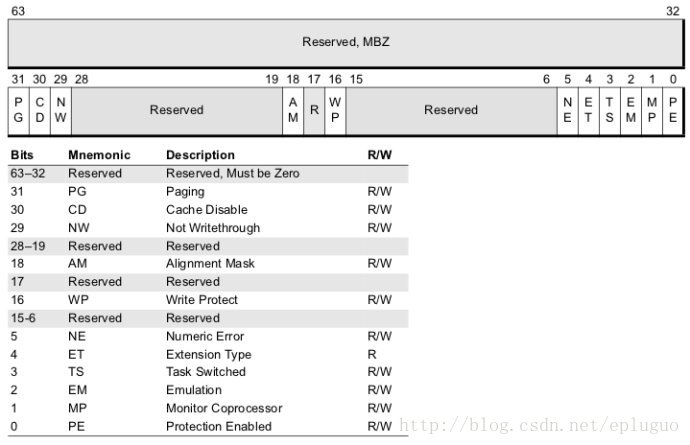
\includegraphics[scale=0.5]{fig/9.jpeg}
\caption{CRO寄存器}
\label{fig:CR0}
\end{figure}
PE: CR0的位0是启用保护(Protection Enable)标志。当设置该位时即开启了保护模式;当复位时即进入实地址模式。这个标志仅开启段级保护,而并没有启用分页机制。若要启用分页机制,那么PE和PG标志都要置位。\\\\
MP: CR0的位1是监控协处理器(Monitor coProcessor或Math Present)标志。用于控制WAIT/FWAIT指令与TS标志的交互作用。如果MP=1、TS=1,那么执行WAIT指令将产生一个设备不存在异常;如果MP=0,则TS标志不会影响WAIT的执行。\\\\
EM:CR0的位2是仿真(EMulation)标志。当该位设置时,表示处理器没有内部或外部协处理器,执行协处理器指令时会引起设备不存在异常;当清除时,表示系统有协处理器。设置这个标志可以迫使所有浮点指令使用软件来模拟。\\\\
TS:CR0的位3是任务已切换(Task Switched)标志。该标志用于推迟保存任务切换时的协处理器内容,直到新任务开始实际执行协处理器指令。处理器在每次任务切换时都会设置该标志,并且在执行协处理器指令时测试该标志。如果设置了TS标志并且CR0的EM标志为0,那么在执行任何协处理器指令之前会产生一个设备不存在异常。如果设置了TS标志但没有设置CR0的MP和EM标志,那么在执行协处理器指令WAIT/FWAIT之前不会产生设备不存在异常。如果设置了EM标志,那么TS标志对协处理器指令的执行无影响。在任务切换时,处理器并不自动保存协处理器的上下文,而是会设置TS标志。这个标志会使得处理器在执行新任务指令流的任何时候遇到一条协处理器指令时产生设备不存在异常。设备不存在异常的处理程序可使用CLTS指令清除TS标志,并且保存协处理器的上下文。如果任务从没有使用过协处理器,那么相应协处理器上下文就不用保存。\\\\
ET:CR0的位4是扩展类型(Extension Type)标志。当该标志为1时,表示指明系统中有80387协处理器,并使用32位协处理器协议。ET=0指明使用80287协处理器。如果仿真位EM=1,则该位将被忽略。在处理器复位操作时,ET位会被初始化指明系统中使用的协处理器类型。如果系统中有80387,则ET被设置成1,否则若有一个80287或者没有协处理器,则ET被设置成0。\\\\
NE:对于Intel 80486或以上的CPU,CR0的位5是协处理器错误(Numeric Error)标志。当设置该标志时,就启用了x87协处理器错误的内部报告机制;若复位该标志,那么就使用PC形式的x87协处理器错误报告机制。当NE为复位状态并且CPU的IGNNE输入引脚有信号时,那么数学协处理器x87错误将被忽略。当NE为复位状态并且CPU的IGNNE输入引脚无信号时,那么非屏蔽的数学协处理器x87错误将导致处理器通过FERR引脚在外部产生一个中断,并且在执行下一个等待形式浮点指令或WAIT/FWAIT指令之前立刻停止指令执行。CPU的FERR引脚用于仿真外部协处理器80387的ERROR引脚,因此通常连接到中断控制器输入请求引脚上。NE标志、IGNNE引脚和FERR引脚用于利用外部逻辑来实现PC形式的外部错误报告机制。\\\\
WP:对于Intel 80486或以上的CPU,CR0的位16是写保护(Write Proctect)标志。当设置该标志时,处理器会禁止超级用户程序(例如特权级0的程序)向用户级只读页面执行写操作;当该位复位时则反之。该标志有利于UNIX类操作系统在创建进程时实现写时复制(Copy on Write)技术。\\\\
PG:CR0的位31是分页(Paging)标志。当设置该位时即开启了分页机制;当复位时则禁止分页机制,此时所有线性地址等同于物理地址。在开启这个标志之前必须已经或者同时开启PE标志。当改变PE和PG位时,必须小心。只有当执行程序至少有部分代码和数据在线性地址空间和物理地址空间中具有相同地址时,我们才能改变PG位的设置。此时这部分具有相同地址的代码在分页和未分页世界之间起着桥梁的作用。无论是否开启分页机制,这部分代码都具有相同的地址。另外,在开启分页(PG=1)之前必须先刷新页高速缓冲TLB。在修改该了PE位之后程序必须立刻使用一条跳转指令,以刷新处理器执行管道中已经获取的不同模式下的任何指令。在设置PE位之前,程序必须初始化几个系统段和控制寄存器。在系统刚上电时,处理器被复位成PE=0和PG=0(即实模式状态),以允许引导代码在启用分段和分页机制之前能够初始化这些寄存器和数据结构。
\begin{lstlisting}[breaklines]
	movl %cr0,%eax # check math chip
	andl $0x80000011,%eax # Save PG,ET,PE
	testl $0x10,%eax
	jne 1f # ET is set - 387 is present
	orl $4,%eax	# else set emulate bit
1:	movl %eax,%cr0
\end{lstlisting}
\subsubsection{跳转到页表之后}	
\paragraph{•}
为什么要跳到页表建立之后呢?
\begin{lstlisting}[breaklines]
	jmp after_page_tables
\end{lstlisting}
\subsubsection{子程序1, 建立idt}	
\paragraph{•}
IDT表最大有256个门描述符,setup\_idt子程序,将256项中都设置中断处理函数为ignore\_int,然后用lidt加载IDT表。其中EAX:0x00080000中,高位的0x0008(0b1000)1为索引,0表示GDT,RPL=00表示最高优先级;低位的0x0000随后被置为ignore\_int。由于ignore\_int偏移的高位部分均为0,只需要处理高32bit中的低16bit,DX:0x8e00,其中0xe=0b1110,表示描述符为中断描述符;0x8=0b1000,即P=1,表示段存在标记;DPL=00,表示访问限制在内核态。
\begin{lstlisting}[breaklines]
setup_idt:
	lea ignore_int,%edx
	movl $0x00080000,%eax
	movw %dx,%ax /* selector = 0x0008 = cs */
	movw $0x8E00,%dx /* interrupt gate - dpl=0, present */

	lea idt,%edi
	mov $256,%ecx
rp_sidt:
	movl %eax,(%edi)
	movl %edx,4(%edi)
	addl $8,%edi
	dec %ecx
	jne rp_sidt
	lidt idt_descr
	ret
\end{lstlisting}
\subsubsection{子程序2, 建立gdt}	
GDT表后面会在init.s中被重写,这里只有两项,在gdt\_descr指向的区域描述。
\begin{lstlisting}[breaklines]
setup_gdt:
	lgdt gdt_descr
	ret
\end{lstlisting}
\subsubsection{页表空间}	
内核的页目录从0地址开始,在head.s最开始用pg\_dir定义。这里使用pg0到pg2定义了3个表,每个页表长为4 Kb 字节,而每个页表项需要4 个字节,因此一个页表共可以存放1024个表项。一个页表项寻址4 Kb 的地址空间,则一个页表就可以寻址4 Mb 的物理内存。这里定义了3个页表,最大可以寻址到12Mb的物理内存。
\begin{lstlisting}[breaklines]
.org 0x1000
pg0:

.org 0x2000
pg1:

.org 0x3000
pg2: # This is not used yet, but if you
 # want to expand past 8 Mb, you'll have
 # to use it.
 .org 0x4000
\end{lstlisting}
\subsubsection{准备到main的对栈}	
setup\_paging看起来是一个函数,但这里是跳转到setup\_paging而不是通过函数调用,利用setup\_paging的返回,直接返回到main函数。
\begin{lstlisting}[breaklines]
after_page_tables:
	pushl $0 # These are the parameters to main :-)
	pushl $0
	pushl $0
	pushl $L6 # return address for main, if it decides to.
	pushl $_main
	jmp setup_paging
L6:
	jmp L6 # main should never return here, but
 # just in case, we know what happens.
\end{lstlisting}
\subsubsection{子程序3, 缺省的中断处理函数}	
用直接写显存的方式,显示一个字符。
\begin{lstlisting}[breaklines]
.align 2
ignore_int:
	incb 0xb8000+160 # put something on the screen
	movb $2,0xb8000+161	# so that we know something
	iret # happened
\end{lstlisting}
\subsubsection{建立页表, 返回到main函数}	
cld设置edi或同esi为递增方向,rep做(\%ecx)次重复操作,stosl表示edi每次增加4,cld;rep;stosl这条语句达到按4字节清空前3*1024*4字节地址空间的目的。\\\\
pg\_dir从0开始,从0到pg0(0x1000)之间的内存是留给页目录的。
页目录项的结构4 个字节为1 项。格式为:
\begin{list}{•}{•}
\item 前0-11 位存放标志,例如是否在内存中(P 位0)、读写许可(R/W 位1)、普通用户还是超级用户使用(U/S 位2)、PWT 位3、PCD 位4、是否被访问过 位5、是否修改过(是否脏了)(D 位6)等;
\item 表项的位12-31 是页框地址,用于指出一页内存的物理起始地址。
\end{list}
\begin{figure}[htbp]
\centering
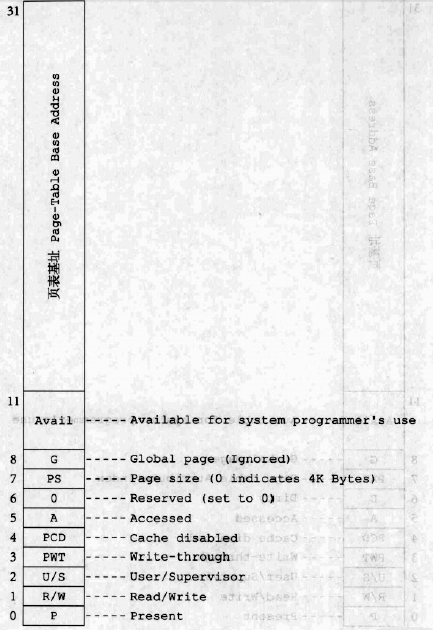
\includegraphics[scale=0.5]{fig/10.png}
\caption{页目录项结构}
\label{fig:PDE}
\end{figure}
目录项只有pg0和pg1两个,"\$pg0+7"表示:0x00001007,第1 个页表所在的地址 = 0x00001007 \& 0xfffff000 = 0x1000;第1 个页表的属性标志 = 0x00001007 \& 0x00000fff = 0x07,表示该页存在、用户可读写。\\\\
然后,从pg1的最后一个表项开始,往回填充。其中0x000007为标志位,和目录项类似,稍有不同。前20位同样为该表项对应的物理内存的地址,每个表项以4k,即0x1000为间隔。
\begin{figure}[htbp]
\centering
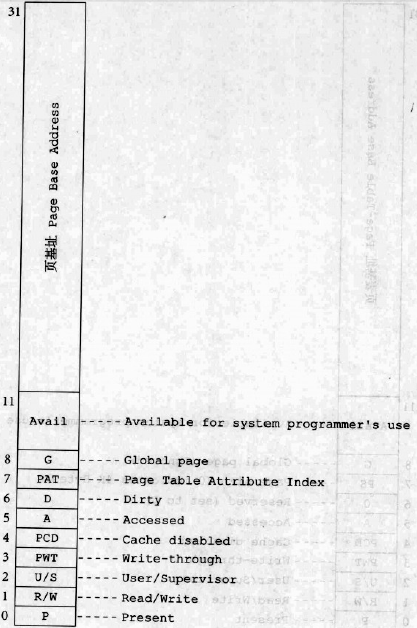
\includegraphics[scale=0.5]{fig/11.png}
\caption{页表项结构}
\label{fig:PTE}
\end{figure}
cr3又叫PDBR,它的高20位是页目录表首地址的高20位(低12为零,即页目录表会是4KB对齐的)。其第3bit为PWT (Write-through) 标记,第4bit为PCD (Cache Disabled) 标记。
\begin{lstlisting}[breaklines]
.align 2
setup_paging:
	movl $1024*3,%ecx
	xorl %eax,%eax
	xorl %edi,%edi /* pg_dir is at 0x000 */
	cld;rep;stosl
	movl $pg0+7,_pg_dir /* set present bit/user r/w */
	movl $pg1+7,_pg_dir+4 /*  --------- " " --------- */
	movl $pg1+4092,%edi
	movl $0x7ff007,%eax /*  8Mb - 4096 + 7 (r/w user,p) */
	std
1:	stosl /* fill pages backwards - more efficient :-) */
	subl $0x1000,%eax
	jge 1b
	xorl %eax,%eax /* pg_dir is at 0x0000 */
	movl %eax,%cr3 /* cr3 - page directory start */
	movl %cr0,%eax
	orl $0x80000000,%eax
	movl %eax,%cr0 /* set paging (PG) bit */
	ret	 /* this also flushes prefetch-queue */	
\end{lstlisting}
\subsubsection{idt, gdt描述符和表项空间}	
idt, gdt描述符和表项空间和内核0.00类似,这里不再赘述。
\begin{lstlisting}[breaklines]
.align 2
.word 0
idt_descr:
	.word 256*8-1 # idt contains 256 entries
	.long idt
.align 2
.word 0
gdt_descr:
	.word 256*8-1 # so does gdt (not that that's any
	.long gdt # magic number, but it works for me :^)

	.align 8 
idt:	.fill 256,8,0 # idt is uninitialized

gdt:
	.quad 0x0000000000000000 /* NULL descriptor */
	.quad 0x00c09a00000007ff /* 8Mb */
	.quad 0x00c09200000007ff /* 8Mb */
	.quad 0x0000000000000000 /* don't use */
	.fill 252,8,0 /*for LDT's and TSS's etc */
\end{lstlisting}
\subsubsection{stack\_start在那里?}	
\part{init目录}
init目录下面只有一个main.c。 系统在执行完boot目录下的head.s后,通过一个ret指令将执行权交给main.c中的main函数,完成内核初始化的所有工作。
\section{main.c}
这是我们遇到的一个C程序,远比汇编程序复杂,不能再像看汇编代码那样一步步顺序往前看。更便于理解的方式是从主流程上向各分支扩展。\\
main.c首先确定如何分配使用系统的物理内存,然后调用内核各部分的初始化函数分别对内存管理、中断处理、块设备和字符设备、进程管理以及硬盘和软盘硬件进行初始化。在完成了这些操作之后,程序手工吧自己移动到任务0中运行,并使用fork创建出进程1,并在其中调用init函数,继续进行应用化境的初始化并执行shell登录程序。原进程0则在系统空闲时被调度执行。
\subsection{main函数}
在head.s的最后,通过setup\_paging的返回,将控制权交给了main。在main中,首先进行了一系列的初始化,然后开中断,进入到用户态,然后通过fork创建子进程,在子进程中调用init()。在init的最后,通过\_exit退出。父进程则进入pause。
\begin{lstlisting}[breaklines]
void main(void)
{
	time_init();
	tty_init();
	trap_init();
	sched_init();
	buffer_init();
	hd_init();
	sti();
	move_to_user_mode();
	if (!fork()) {
		init();
	}
	for(;;) pause();
}
\end{lstlisting}
\subsubsection{理解fork的处理}
复刻(英语:fork,又译作派生、分支)是UNIX或类UNIX中的分叉函数,fork函数将运行着的程序分成2个(几乎)完全一样的进程,每个进程都启动一个从代码的同一位置开始执行的线程。这两个进程中的线程继续执行,就像是两个用户同时启动了该应用程序的两个副本。\\
新进程,称为子进程,它与进程(称为系统调用fork的进程)同时运行,此进程称为父进程。创建新的子进程后,两个进程将执行fork()系统调用之后的下一条指令。子进程使用相同的pc(程序计数器),相同的CPU寄存器,在父进程中使用的相同打开文件。\\
调用fork之后,数据、堆、栈有两份,代码仍然为一份。这个代码段成为两个进程的共享代码段,都从fork函数中返回,箭头表示各自的执行处。当父子进程有一个想要修改数据或者堆栈时,两个进程真正分裂。由于在复制时复制了父进程的堆栈段,所以两个进程都停留在fork函数中,等待返回。因此fork函数会返回两次,一次是在父进程中返回,另一次是在子进程中返回,这两次的返回值是不一样的。两次返回区别是子进程中返回0值而父进程中返回子进程ID。我们可以通过fork返回的值来判断当前进程是子进程还是父进程。
\begin{lstlisting}[breaklines]
	if (!fork()) {
		init();
	}
\end{lstlisting}
上面代码中对fork返回值的判断,说明init函数只在子进程中被调用。
\subsubsection{理解Copy-on-write}	
写入时复制(英语:Copy-on-write,简称COW)核心思想是,如果有多个调用者(callers)同时请求相同资源(如内存或磁盘上的数据存储),他们会共同获取相同的指针指向相同的资源,直到某个调用者试图修改资源的内容时,系统才会真正复制一份专用副本(private copy)给该调用者,而其他调用者所见到的最初的资源仍然保持不变。这过程对其他的调用者都是透明的(transparently)。优点是如果调用者没有修改该资源,就不会有副本(private copy)被建立,因此多个调用者只是读取操作时可以共享同一份资源。\\
在Linux程序中,fork()会产生一个和父进程完全相同的子进程,出于效率考虑,linux中引入了“写时复制“技术,也就是只有进程空间的各段的内容要发生变化时,才会将父进程的内容复制一份给子进程。在fork之后两个进程用的是相同的物理空间(内存区),子进程的代码段、数据段、堆栈都是指向父进程的物理空间,也就是说,两者的虚拟空间不同,但其对应的物理空间是同一个。当父子进程中有更改相应段的行为发生时,再为子进程相应的段分配物理空间。
\subsubsection{宏和内联函数定义}	
Linux在内核空间创建进程时不使用写时复制技术(意味着代码段、数据段、堆栈段是独立空间,都复制一份?)。main()在从内核态移动到用户态(任务0)后,父进程和子进程的堆栈中都会保留调用fork的痕迹。通过将fork函数定义为内联函数,可以让堆栈干净。\\
定义LIBRARY宏的目的是为了使用在include目录下的unistd.h中的内嵌汇编代码。
\begin{lstlisting}
#define __LIBRARY__
#include <unistd.h>
#include <time.h>

static inline _syscall0(int,fork)
static inline _syscall0(int,pause)
static inline _syscall0(int,setup)
static inline _syscall0(int,sync)
\end{lstlisting}
其中,\_syscall0为一个宏,在unistd.h中定义为:
\begin{lstlisting}
#define _syscall0(type,name) \
type name(void) \
{ \
type __res; \
__asm__ volatile ("int $0x80" \
	: "=a" (__res) \
	: "0" (__NR_##name)); \
if (__res >= 0) \
	return __res; \
errno = -__res; \
return -1; \
}
\end{lstlisting}
c语言里,\#把宏参数变为一个字符串,\#\#把两个宏参数贴合在一起。以fork为例,在main.c中的定义,就会被替换为:
\begin{lstlisting}
static inline int fork(void) \
{ \
int __res; \
__asm__ volatile ("int $0x80" \
	: "=a" (__res) \
	: "0" (__NR_fork)); \
if (__res >= 0) \
	return __res; \
errno = -__res; \
return -1; \
}
\end{lstlisting}
GCC 支持在C/C++代码中嵌入汇编代码,这些汇编代码被称作GCC Inline ASM——GCC内联汇编。基本内联汇编的格式是:\\\\
\begin{lstlisting}
__asm__ __volatile__("Instruction List");
\end{lstlisting}
\_\_asm\_\_是GCC关键字asm的宏定义;\\
\_\_volatile\_\_ 或volatile是可选的,你可以用它也可以不用它。如果你用了它,则是向GCC声明“不要动我所写的Instruction List,我需要原封不动的保留每一条指令”,否则当你使用了优化选项(-O)进行编译时,GCC将会根据自己的判断决定是否将这个内联汇编表达式中的指 令优化掉;\\
Instruction List是汇编指令序列, 任意两个指令间要么被分号(;)分开,要么被放在两行; \\\\
带有C/C++表达式的内联汇编格式为:
\begin{lstlisting}[breaklines]
__asm__ __volatile__("Instruction List" : Output : Input : Clobber/Modify)
\end{lstlisting}
此时"Instruction List"中的寄存器写法要遵守相关规定,比如寄存器前必须使用两个百分号(\%\%),而不是像基本汇编格式一样在寄存器前只使用一个百分号(\%)。\\
Output: "=a" (\_\_res),它包含两个约束:等号(=)和字母a,其中等号(=)说明括号中左值表达式\_\_res是一个 Write-Only的,只能够被作为当前内联汇编的输入,而不能作为输入。而字母a是寄存器EAX / AX / AL的简写,说明\_\_res的值要从eax寄存器中获取,也就是说\_\_res = eax \\
Input: "0" (\_\_NR\_\#\#name)),引号中的部分是约束部分,和输出表达式约束不同的是,它不允许指定加号(+)约束和等号(=)约束,也就是说它只能是默认的Read-Only的。数字0,1,2,3,4,5,6,7,8,9 I 表示和第n个操作表达式使用相同的寄存器/内存。\_\_NR\_fork则在unistd.h中定义为2。\\
Clobber/Modify:有时候,你想通知GCC当前内联汇编语句可能会对某些寄存器或内存进行修改,希望GCC在编译时能够将这一点考虑进去。那么你就可以在Clobber/Modify域声明这些寄存器或内存。如果你在一个内联汇编语句的Clobber/Modify域向GCC声明某个寄存器内容发生了改变,GCC在编译时,如果发现这个被声明的寄存器的内容在此 内联汇编语句之后还要继续使用,那么GCC会首先将此寄存器的内容保存起来,然后在此内联汇编语句的相关生成代码之后,再将其内容恢复。
\subsection{time\_init函数}	
time\_init函数读取CMOS时间,并将其转换到startup\_time中。这里循环读取CMOS时间,判断连续2次的读取结果的一致性,避免在时间眺变,如果满60s时,min值改变出错?
\begin{lstlisting}[breaklines]
extern long kernel_mktime(struct tm * tm);
extern long startup_time;

#define CMOS_READ(addr) ({ \
outb_p(0x80|addr,0x70); \
inb_p(0x71); \
})

#define BCD_TO_BIN(val) ((val)=((val)&15) + ((val)>>4)*10)

static void time_init(void)
{
	struct tm time;

	do {
		time.tm_sec = CMOS_READ(0);
		time.tm_min = CMOS_READ(2);
		time.tm_hour = CMOS_READ(4);
		time.tm_mday = CMOS_READ(7);
		time.tm_mon = CMOS_READ(8)-1;
		time.tm_year = CMOS_READ(9);
	} while (time.tm_sec != CMOS_READ(0));
	BCD_TO_BIN(time.tm_sec);
	BCD_TO_BIN(time.tm_min);
	BCD_TO_BIN(time.tm_hour);
	BCD_TO_BIN(time.tm_mday);
	BCD_TO_BIN(time.tm_mon);
	BCD_TO_BIN(time.tm_year);
	startup_time = kernel_mktime(&time);
}
\end{lstlisting}
\subsection{tty\_init函数}
终端是一种字符型设备,它有多种类型。我们通常使用tty来简称各种类型的终端设备。tty是Teletype的缩写,Teletype是一种由Teletype公司生产的最早出现的终端设备,样子很象电传打字机。现在的终端设备可以分为以下几种类型:
\begin{enumerate}
\item 串行端口终端:计算机把每个串行端口都看作是一个字符设备。
\item 伪终端:功能类似与终端设备,但不与硬件相关,如通过网络登录主机时,为网络服务器和登录shenll程序之前提供一个终端接口。
\item 控制终端:进程的控制终端。
\item 控制台:计算机显示器通常被称为控制台终端或控制台。
\item 其他类型
\end{enumerate}
在Linux 0.01系统中可以使用两类终端。一类是主机上的控制台终端,另一类是串行硬件终端设备。
\begin{lstlisting}[breaklines]
void tty_init(void)
{
	rs_init();
	con_init();
}
\end{lstlisting}
\subsubsection{rs\_init函数}
串行接口 (Serial Interface)是指数据一位一位地顺序传送。其特点是通信线路简单,只要一对传输线就可以实现双向通信(可以直接利用电话线作为传输线),PC机上通常有2个符合RS-232C标准的串行接口,并使用异步接收/发送控制芯片UART(Universal Asynchronous Receiver/Transmitter)来处理串行数据的收发。rs\_init在kernel下的serial.c中
\begin{lstlisting}[breaklines]
void rs_init(void)
{
	set_intr_gate(0x24,rs1_interrupt);
	set_intr_gate(0x23,rs2_interrupt);
	init(tty_table[1].read_q.data);
	init(tty_table[2].read_q.data);
	outb(inb_p(0x21)&0xE7,0x21);
}
\end{lstlisting}
\paragraph{设置两个串口对应中断处理函数}
在boot.s中,已通过ICW2的设置,将主片中断请求0~7级对应的中断号设置为0x20~0x27;从片的ICW2设置成 0x28,表示从片中断请求8~15级对应的中断号是 0x28~0x2f。因此,和两个串口对应的IRQ3和IRQ4,中断号为0x23和0x24。set\_intr\_gate在include目录下的asm子目录中的system.h中定义。
\paragraph{tty\_table[]的定义}
在tty\_io.c中,一共定义了3个tty\_struct,其中tty\_table[0]对应控制台终端,tty\_table[1]和tty\_table[2]分别对应rs1和rs2.
\begin{lstlisting}[breaklines]
struct tty_struct tty_table[] = {
	{
		{0,
		OPOST|ONLCR,/* change outgoing NL to CRNL */
		0,
		ICANON | ECHO | ECHOCTL | ECHOKE,
		0,/* console termio */
		INIT_C_CC},
		0,/* initial pgrp */
		0,/* initial stopped */
		con_write,
		{0,0,0,0,""},/* console read-queue */
		{0,0,0,0,""},/* console write-queue */
		{0,0,0,0,""}/* console secondary queue */
	},{
		{0, /*IGNCR*/
		OPOST | ONLRET,	/* change outgoing NL to CR */
		B2400 | CS8,
		0,
		0,
		INIT_C_CC},
		0,
		0,
		rs_write,
		{0x3f8,0,0,0,""},/* rs 1 */
		{0x3f8,0,0,0,""},
		{0,0,0,0,""}
	},{
		{0, /*IGNCR*/
		OPOST | ONLRET,	/* change outgoing NL to CR */
		B2400 | CS8,
		0,
		0,
		INIT_C_CC},
		0,
		0,
		rs_write,
		{0x2f8,0,0,0,""},/* rs 2 */
		{0x2f8,0,0,0,""},
		{0,0,0,0,""}
	}
};
\end{lstlisting}
\paragraph{tty\_struct和tty\_queue的定义}
tty\_struct在tty.h中定义\\
\begin{lstlisting}[breaklines]
struct tty_struct {
	struct termios termios;
	int pgrp;
	int stopped;
	void (*write)(struct tty_struct * tty);
	struct tty_queue read_q;
	struct tty_queue write_q;
	struct tty_queue secondary;
	};
\end{lstlisting}
tty\_queue在tty.h中定义.\\
\begin{lstlisting}[breaklines]
struct tty_queue {
	unsigned long data;
	unsigned long head;
	unsigned long tail;
	struct task_struct * proc_list;
	char buf[TTY_BUF_SIZE];
};
\end{lstlisting}
read\_q.data在tty\_table[]全局变量中已经定义好\\
tty\_table[1].read\_q.data = 0x3f8,对应rs1端口\\
tty\_table[2].read\_q.data = 0x2f8,对应rs2端口
\paragraph{初始化对应的端口}
与终端控制芯片8259A一样,URAT也是一个可编程的控制芯片。通过对其内部寄存器进行设置,可以设置串行通信的工作参数和UART的工作方式。以rs1为例:
\begin{enumerate}
\item 通过0x3fb端口,写线路控制寄存器LCR,bit7为1是允许访问除数锁存寄存器DLAB=1。
\item 通过0x3f8端口,读/写波特率因子低字节,0x30对应48,UART时钟频率1843200/48/16=2400bps。
\item 通过0x3f9端口,读/写波特率因子高字节,0x0。
\item 通过0x3fb端口,写线路控制寄存器LCR,bit7为0清空除数锁存访问位,bit1-0为0b11,表示8位数据位。
\item 通过0x3fc端口,bit3=1设置为中断方式,bit1-0=11设置为数据终端就绪和请求发送。
\item 通过0x3f8端口,DLAB=0, bit3=1 Modem状态允许中断,bit2=1 接收线路允许中断, bit0=1 接收到数据允许中断, bit1=0 当前没有数据发送,不允许中断。
\end{enumerate}
\begin{lstlisting}[breaklines]
static void init(int port)
{
	outb_p(0x80,port+3);/* set DLAB of line control reg */
	outb_p(0x30,port);/* LS of divisor (48 -> 2400 bps */
	outb_p(0x00,port+1);/* MS of divisor */
	outb_p(0x03,port+3);/* reset DLAB */
	outb_p(0x0b,port+4);/* set DTR,RTS, OUT_2 */
	outb_p(0x0d,port+1);/* enable all intrs but writes */
	(void)inb(port);/* read data port to reset things (?) */
}
\end{lstlisting}
其中的outb\_p为带有延时的outb操作,inb不带延时,均在io.h中定义。最后一个读串口的操作,但没有对结果进行处理。
\paragraph{允许IRQ3和IRQ4中断}
通过inb\_p(0x21),读出8259A的OCW, 和0xe7与操作, 将OCW的bit3和bit4置0,允许中断。

\subsubsection{con\_init函数}
另一类要激活的是主机上的控制台终端,在文件console.c中;
\begin{lstlisting}[breaklines]
void con_init(void)
{
	register unsigned char a;

	gotoxy(*(unsigned char *)(0x90000+510),*(unsigned char *)(0x90000+511));
	set_trap_gate(0x21,&keyboard_interrupt);
	outb_p(inb_p(0x21)&0xfd,0x21);
	a=inb_p(0x61);
	outb_p(a|0x80,0x61);
	outb(a,0x61);
}
\end{lstlisting}
\paragraph{保存屏幕光标位置}
boot.s中,把当前光标位置,保存在内存0x90510处。con\_init首先通过gotoxy函数,把boot.s中保存在内存0x90510处的当前光标位置保存在console.c的全局变量x,y中。
\begin{lstlisting}[breaklines]
	mov	ah,#0x03	| read cursor pos
	xor	bh,bh
	int	0x10		| save it in known place, con_init fetches
	mov	[510],dx	| it from 0x90510.
\end{lstlisting}
gotoxy函数,更新console.c的全局变量x,y。
\begin{lstlisting}[breaklines]
static inline void gotoxy(unsigned int new_x,unsigned int new_y)
{
	if (new_x>=columns || new_y>=lines)
		return;
	x=new_x;
	y=new_y;
	pos=origin+((y*columns+x)<<1);
}
\end{lstlisting}
\paragraph{设置键盘中断处理函数} set\_trap\_gate将0x21号中断设置为键盘处理函数;这里设置为陷井门可能是出于几个考虑:\\
1. 若设置为中断门,则中断允许标志IF会被置为0,即中断处理过程中cpu不允许响应其他中断请求。而对于控制台终端而言,响应键盘处理应该是一种常用操作,不需要将IF置位;\\
2. 陷阱处理程序提供的服务为当前进程所用,而中断处理程序的服务不是为了当前进程的。\\
3. 在boot.s中,已通过ICW2的设置,将主片中断请求0~7级对应的中断号设置为0x20~0x27;从片的ICW2设置成 0x28,表示从片中断请求8~15级对应的中断号是 0x28~0x2f。因此,IRQ1对应的中断号即为0x21。
\paragraph{允许主8259A响应IRQ1的中断请求} 
通过inb\_p(0x21),读出8259A的OCW, 和0xfd与操作, 将OCW的bit1置0,允许中断。
\paragraph{复位键盘} 通过0x61端口读入键盘状态,设置禁止单板工作,然后再恢复,起到复位键盘的作用。61H早期用于8255B口,bit 7用于应答键盘(仅早期pc机),bit 0~1用于开关8253/4输出到SPEAKER,其他的位不要去动。
\subsection{trap\_init函数}	
在文件traps.c中,设置中断向量表,可以看到0~17号中断向量被设置为对应的异常处理函数,3~5可以被用户态调用,17~31保留。(上节中我们看到35/36被串口IRQ3/4占用,33被IRQ1,键盘中断占用)
\begin{lstlisting}[breaklines]
void trap_init(void)
{
	int i;

	set_trap_gate(0,&divide_error);
	set_trap_gate(1,&debug);
	set_trap_gate(2,&nmi);
	set_system_gate(3,&int3);	/* int3-5 can be called from all */
	set_system_gate(4,&overflow);
	set_system_gate(5,&bounds);
	set_trap_gate(6,&invalid_op);
	set_trap_gate(7,&device_not_available);
	set_trap_gate(8,&double_fault);
	set_trap_gate(9,&coprocessor_segment_overrun);
	set_trap_gate(10,&invalid_TSS);
	set_trap_gate(11,&segment_not_present);
	set_trap_gate(12,&stack_segment);
	set_trap_gate(13,&general_protection);
	set_trap_gate(14,&page_fault);
	set_trap_gate(15,&reserved);
	set_trap_gate(16,&coprocessor_error);
	for (i=17;i<32;i++)
		set_trap_gate(i,&reserved);
/*	__asm__("movl $0x3ff000,%%eax\n\t"
		"movl %%eax,%%db0\n\t"
		"movl $0x000d0303,%%eax\n\t"
		"movl %%eax,%%db7"
		:::"ax");*/
}
\end{lstlisting}
\subsection{sched\_init函数}	
在文件sched.c中,linux设置了64个任务,在初始化函数中,设置了每个任务的TSS/LDT,设置了定时器,准备好向TASK[0]切换。

\begin{lstlisting}[breaklines]
void sched_init(void)
{
	int i;
	struct desc_struct * p;

	set_tss_desc(gdt+FIRST_TSS_ENTRY,&(init_task.task.tss));
	set_ldt_desc(gdt+FIRST_LDT_ENTRY,&(init_task.task.ldt));
	p = gdt+2+FIRST_TSS_ENTRY;
	for(i=1;i<NR_TASKS;i++) {
		task[i] = NULL;
		p->a=p->b=0;
		p++;
		p->a=p->b=0;
		p++;
	}
	ltr(0);
	lldt(0);
	outb_p(0x36,0x43);		/* binary, mode 3, LSB/MSB, ch 0 */
	outb_p(LATCH & 0xff , 0x40);	/* LSB */
	outb(LATCH >> 8 , 0x40);	/* MSB */
	set_intr_gate(0x20,&timer_interrupt);
	outb(inb_p(0x21)&~0x01,0x21);
	set_system_gate(0x80,&system_call);
}
\end{lstlisting}
\subsubsection{初始化init\_task}
\paragraph{task相关的数据结构} task[]数组\\
task[NR\_TASKS]为全局变量,定义在sched.c中,NR\_TASKS为64;数组中的task[0]一开始就被初始化,指向全局变量init\_task。
\begin{lstlisting}[breaklines]
struct task_struct * task[NR_TASKS] = {&(init_task.task), };
\end{lstlisting}
\paragraph{task数据结构} task\_union\\
task\_union是定义了stack的task结构。从task\_union的定义可以看到,task和该task的stack共用一个页面的内存空间。init\_task就是这样定义的一个结构。
\begin{lstlisting}[breaklines]
union task_union {
	struct task_struct task;
	char stack[PAGE_SIZE];
};

static union task_union init_task = {INIT_TASK,};
\end{lstlisting}
\paragraph{task数据结构} task\_struct\\
task的结构定义在sched.h中,在每个task中,有一个tss结构,和一个有着3个表项的ldt结构。每个任务的tss和ldt需要注册到GDT表中以完成任务切换。init\_task.task就对应这这样一个结构。
\begin{lstlisting}[breaklines]
struct task_struct {
/* these are hardcoded - don't touch */
	long state;	/* -1 unrunnable, 0 runnable, >0 stopped */
	long counter;
	long priority;
	long signal;
	fn_ptr sig_restorer;
	fn_ptr sig_fn[32];
/* various fields */
	int exit_code;
	unsigned long end_code,end_data,brk,start_stack;
	long pid,father,pgrp,session,leader;
	unsigned short uid,euid,suid;
	unsigned short gid,egid,sgid;
	long alarm;
	long utime,stime,cutime,cstime,start_time;
	unsigned short used_math;
/* file system info */
	int tty;		/* -1 if no tty, so it must be signed */
	unsigned short umask;
	struct m_inode * pwd;
	struct m_inode * root;
	unsigned long close_on_exec;
	struct file * filp[NR_OPEN];
/* ldt for this task 0 - zero 1 - cs 2 - ds&ss */
	struct desc_struct ldt[3];
/* tss for this task */
	struct tss_struct tss;
};
\end{lstlisting}
\paragraph{init\_task.task的初始值} INIT\_TASK\\
在sched.c中:
\begin{lstlisting}[breaklines]
#define INIT_TASK \
/* state etc */	{ 0,15,15, \
/* signals */	0,NULL,{(fn_ptr) 0,}, \
/* ec,brk... */	0,0,0,0,0, \
/* pid etc.. */	0,-1,0,0,0, \
/* uid etc */	0,0,0,0,0,0, \
/* alarm */	0,0,0,0,0,0, \
/* math */	0, \
/* fs info */	-1,0133,NULL,NULL,0, \
/* filp */	{NULL,}, \
	{ \
		{0,0}, \
/* ldt */	{0x9f,0xc0fa00}, \
		{0x9f,0xc0f200}, \
	}, \
/*tss*/	{0,PAGE_SIZE+(long)&init_task,0x10,0,0,0,0,(long)&pg_dir,\
	 0,0,0,0,0,0,0,0, \
	 0,0,0x17,0x17,0x17,0x17,0x17,0x17, \
	 _LDT(0),0x80000000, \
		{} \
	}, \
}
\end{lstlisting}
\paragraph{初始化init\_task.task.tss}
TSS的结构定义在sched.h中\\
\begin{lstlisting}[breaklines]
struct tss_struct {
	long	back_link;	/* 16 high bits zero */
	long	esp0;
	long	ss0;		/* 16 high bits zero */
	long	esp1;
	long	ss1;		/* 16 high bits zero */
	long	esp2;
	long	ss2;		/* 16 high bits zero */
	long	cr3;
	long	eip;
	long	eflags;
	long	eax,ecx,edx,ebx;
	long	esp;
	long	ebp;
	long	esi;
	long	edi;
	long	es;		/* 16 high bits zero */
	long	cs;		/* 16 high bits zero */
	long	ss;		/* 16 high bits zero */
	long	ds;		/* 16 high bits zero */
	long	fs;		/* 16 high bits zero */
	long	gs;		/* 16 high bits zero */
	long	ldt;		/* 16 high bits zero */
	long	trace_bitmap;	/* bits: trace 0, bitmap 16-31 */
	struct i387_struct i387;
};
\end{lstlisting}
结合INIT\_TASK中对TSS初始值的设置,我们可以得到:
\begin{lstlisting}[breaklines]
	long	back_link = 0	
	long	esp0 = PAGE_SIZE+(long)&init_task
	long	ss0 = 0x10		
	long	esp1 = 0
	long	ss1 = 0
	long	esp2 = 0
	long	ss2 = 0
	long	cr3 = (long)&pg_dir
	long	eip = 0
	long	eflags = 0
	long	eax = 0, ecx = 0,edx = 0,ebx = 0;
	long	esp = 0;
	long	ebp = 0;
	long	esi = 0;
	long	edi = 0;
	long	es = 0x17;
	long	cs = 0x17;
	long	ss = 0x17;
	long	ds = 0x17;
	long	fs = 0x17;	
	long	gs = 0x17;	
	long	ldt = _LDT(0);
	long	trace_bitmap = 0x80000000;
	struct i387_struct i387 = {};
\end{lstlisting}
其中,从esp0的设置可以看出,初始任务的堆栈+代码段总共占了一个页面的大小,这个和union结构的定义相对应,对应的段描述符为GDT中的第一个段0x10;而从ss=0x17的设置可以看出,低位0x7表示从初始任务切换到的目标任务时,ss同样是第一个段,但对应在LDT中非在GDT中。
\paragraph{init\_task.task.ldt} ldt[3]\\
一个任务的ldt表里有3项,第一项为0,不使用;第二项指向代码段;第三项指向数据段。
\begin{lstlisting}[breaklines]
ldt[0] = {0,0},
ldt[1] = {0x9f,0xc0fa00},
ldt[2] = {0x9f,0xc0f200}
\end{lstlisting}
\paragraph{ldt[1]}代码段描述符\\
0x0000009f,0x00c0fa00的含义:\\
0x009f,Limit,段长低16bit,对应159;\\
0x0000, 段基地址的低16bit\\
0x00,段基地址的中8bit\\
0xfa, 0b11111010,8bit;\\
p,p=1,表示段在内存中存在\\
dpl,dpl=11,表示非内核特权级\\
s,s=1,表示数据段/代码段\\
type,0b1010,Ebit3 = 1,代码段;Cbit2 = 0,非一致代码段;Rbit1 = 1,表示可读;Abit0 = 0,未被访问。\\
0x0,段长高4位\\
0xC,0b1100
g,g=1,表示长度单位为4k字节\\
d,d=1,表示指令和数据是32位\\
x,未使用,填0\\
avl,保留,填0\\
0x00,基地址高8位
\paragraph{ldt[2]}数据段描述符\\
0x0000009f,0x00c0f200参数的含义:\\
0x009f,Limit,段长低16bit,对应159;\\
0x0000, 段基地址的低16bit\\
0x00,段基地址的中8bit\\
0xf2, 0b11110010,8bit;\\
p,p=1,表示段在内存中存在\\
dpl,dpl=11,表示非内核特权级\\
s,s=1,表示数据段/代码段\\
type,0b0010,Ebit3 = 0,数据段;EDbit2 = 0,向高位生长;Wbit1 = 1,表示可写;Abit0 = 0,未被访问。\\
0x0,段长高4位\\
0xC,0b1100
g,g=1,表示长度单位为4k字节\\
d,d=1,表示指令和数据是32位\\
x,未使用,填0\\
avl,保留,填0\\
0x00,基地址高8位
\subsubsection{初始化其他task}
其他任务的初始化分为3部分:\\
1. task[i]初始化为null;\\
2. task[i]在gdt表中的tss描述符置为0;\\
3. task[i]在gdt表中的ldt描述符置为0;
\begin{lstlisting}[breaklines]
	struct desc_struct * p;
	p = gdt+2+FIRST_TSS_ENTRY;
	for(i=1;i<NR_TASKS;i++) {
		task[i] = NULL;
		p->a=p->b=0;
		p++;
		p->a=p->b=0;
		p++;
	}
\end{lstlisting}
64位的段描述用两个unsigned long表示。
\begin{lstlisting}[breaklines]
typedef struct desc_struct {
	unsigned long a,b;
} desc_table[256];
\end{lstlisting}
\subsubsection{加载tss和ldt,准备切换到task[0]}
\begin{lstlisting}[breaklines]
	ltr(0);
	lldt(0);
\end{lstlisting}
通过任务号,得到GDT表中对应描述符的索引,加载task[0]的tss和ldt,准备切换到task[0]
\begin{lstlisting}[breaklines]
#define FIRST_TSS_ENTRY 4
#define FIRST_LDT_ENTRY (FIRST_TSS_ENTRY+1)
#define _TSS(n) ((((unsigned long) n)<<4)+(FIRST_TSS_ENTRY<<3))
#define _LDT(n) ((((unsigned long) n)<<4)+(FIRST_LDT_ENTRY<<3))
#define ltr(n) __asm__("ltr %%ax"::"a" (_TSS(n)))
#define lldt(n) __asm__("lldt %%ax"::"a" (_LDT(n)))
\end{lstlisting}
\subsubsection{初始化定时器,设置时钟中断IRQ0}
PC默认分配给8253三个计数器的端口地址分别为40H~42H,控制字寄存器的端口址为43H。首先通过43H,设置通道0以读写16位的方式、工作在方式3、计数器值采用二进制,控制字为0b00110110 (0x36)。然后向计数器通道0(40H)写入计数器初始值。
\begin{lstlisting}[breaklines]
	outb_p(0x36,0x43);		/* binary, mode 3, LSB/MSB, ch 0 */
	outb_p(LATCH & 0xff , 0x40);	/* LSB */
	outb(LATCH >> 8 , 0x40);	/* MSB */
	set_intr_gate(0x20,&timer_interrupt);
	
#define LATCH (1193180/HZ)
#define HZ 100	
\end{lstlisting}
在trap\_init中,0~17号中断向量被设置为对应的异常处理函数,3~5可以被用户态调用,17~31保留。在tty\_init中35/36被串口IRQ3/4占用,33被IRQ1,键盘中断占用; 这里将0x20,即32 IRQ0设置为定时器中断。
\subsubsection{使能IRQ0外所有中断,初始化系统调用}
\begin{lstlisting}[breaklines]
	outb(inb_p(0x21)&~0x01,0x21);
	set_system_gate(0x80,&system_call);
\end{lstlisting}	
\subsection{buffer\_init函数}
buffer.c位于fs目录下,用于对缓冲区进行操作和管理。缓冲区位于内核代码块和主内存区之间。缓冲区在块设备和内核程序之间起着一个桥梁的作用。除了块设备驱动程序以外,内核程序如果需要访问块设备中的数据,就都需要经过缓冲区间接地操作。
\begin{lstlisting}[breaklines]
void buffer_init(void)
{
	struct buffer_head * h = start_buffer;
	void * b = (void *) BUFFER_END;
	int i;

	while ( (b -= BLOCK_SIZE) >= ((void *) (h+1)) ) {
		h->b_dev = 0;
		h->b_dirt = 0;
		h->b_count = 0;
		h->b_lock = 0;
		h->b_uptodate = 0;
		h->b_wait = NULL;
		h->b_next = NULL;
		h->b_prev = NULL;
		h->b_data = (char *) b;
		h->b_prev_free = h-1;
		h->b_next_free = h+1;
		h++;
		NR_BUFFERS++;
		if (b == (void *) 0x100000)
			b = (void *) 0xA0000;
	}
	h--;
	free_list = start_buffer;
	free_list->b_prev_free = h;
	h->b_next_free = free_list;
	for (i=0;i<NR_HASH;i++)
		hash_table[i]=NULL;
}	
\end{lstlisting}	
\subsubsection{buffer的空间}
buffer的起点是内核代码块的结束点,该点保存在内核模块链接期间由链接程序ld生成外部变量end中。
\begin{lstlisting}[breaklines]
extern int end;
struct buffer_head * start_buffer = (struct buffer_head *) &end;

#define BUFFER_END 0x200000
#define BLOCK_SIZE 1024
\end{lstlisting}	
从start\_buffer开始,保存buffer\_head结构类型,该结构中的b\_data指向数据缓冲块,每个缓冲块大小是1024字节。缓冲块从0x200000反向分配,每分配一个缓冲块,就分配有一个buffer\_head结构与之对应。中间跳过0xA0000到0x100000的显存和BIOS ROM区段,直到buffer\_head结构和缓冲块把buffer区的内存分配完,缓冲块的数量保存在NR\_BUFFERS中。
\subsubsection{hash表}
为了能够快速而有效地在缓冲区判断出请求的数据块是佛已经被读入到缓冲区,buffer使用了有307项的hash表。hash表使用的散列函数由设备号和逻辑块号通过异或操作组合,然后mode 307。buffer\_head中的b\_prev和b\_next就是用于hash表中散列到同一项的多个缓冲块的双向链接。
\begin{lstlisting}[breaklines]
#define NR_HASH 307
\end{lstlisting}	
\subsection{hd\_init函数}
\begin{lstlisting}[breaklines]
void hd_init(void)
{
	int i;

	for (i=0 ; i<NR_REQUEST ; i++) {
		request[i].hd = -1;
		request[i].next = NULL;
	}
	for (i=0 ; i<NR_HD ; i++) {
		hd[i*5].start_sect = 0;
		hd[i*5].nr_sects = hd_info[i].head*
				hd_info[i].sect*hd_info[i].cyl;
	}
	set_trap_gate(0x2E,&hd_interrupt);
	outb_p(inb_p(0x21)&0xfb,0x21);
	outb(inb_p(0xA1)&0xbf,0xA1);
}	
\end{lstlisting}	
\subsubsection{request结构}
request结构保存了最多32组硬盘访问请求。
\begin{lstlisting}[breaklines]
static struct hd_request {
	int hd;		/* -1 if no request */
	int nsector;
	int sector;
	int head;
	int cyl;
	int cmd;
	int errors;
	struct buffer_head * bh;
	struct hd_request * next;
} request[NR_REQUEST];

#define NR_REQUEST	32
\end{lstlisting}	
\subsubsection{hd\_struct结构}
当前最大只支持2块硬盘,通过hd\_struct结构,将硬盘归一化成起始扇区和总扇区数。
\begin{lstlisting}[breaklines]
static struct hd_i_struct{
	int head,sect,cyl,wpcom,lzone,ctl;
	} hd_info[]= { HD_TYPE };

#define NR_HD ((sizeof (hd_info))/(sizeof (struct hd_i_struct)))

static struct hd_struct {
	long start_sect;
	long nr_sects;
} hd[5*MAX_HD]={{0,0},};

#define MAX_HD		2
\end{lstlisting}	
hd\_info[0]默认初始化了一种硬盘结构
\begin{lstlisting}[breaklines]
#if	defined(LASU_HD)
#define HD_TYPE { 7,35,915,65536,920,0 }
#elif	defined(LINUS_HD)
#define HD_TYPE { 5,17,980,300,980,0 },{ 5,17,980,300,980,0 }
#else
#error "must define a hard-disk type"
#endif
\end{lstlisting}	
\subsubsection{设置硬盘中断}
设置硬盘中断处理类型为陷井门(不屏蔽中断)。同时,清除中断控制器的屏蔽位,由于硬盘中断连接在8259A的从片上,所以需要两条语句分别对应端口0x21和0xA1。
\subsection{sti函数}	
使处理器可以响应中断
\begin{lstlisting}[breaklines]
#define sti() __asm__ ("sti"::)
\end{lstlisting}	
\subsection{move\_to\_user\_mode函数}
定义在system.h中,模拟中断调用的返回过程,实现特权的变更和堆栈的切换。把CPU执行控制流移动到初始任务task[0]的环境中。\\\\
iret之前的堆栈操作,用于切换到正确的控制流;iret之后,由于特权变更,需要重新加载正确的段寄存器。
\begin{lstlisting}[breaklines]
#define move_to_user_mode() \
__asm__ ("movl %%esp,%%eax\n\t" \
	"pushl $0x17\n\t" \
	"pushl %%eax\n\t" \
	"pushfl\n\t" \
	"pushl $0x0f\n\t" \
	"pushl $1f\n\t" \
	"iret\n" \
	"1:\tmovl $0x17,%%eax\n\t" \
	"movw %%ax,%%ds\n\t" \
	"movw %%ax,%%es\n\t" \
	"movw %%ax,%%fs\n\t" \
	"movw %%ax,%%gs" \
	:::"ax")
\end{lstlisting}	
\subsection{fork函数}	
fork函数复制正在运行的任务,由于在复制时复制了父进程的堆栈段,所以父子两个进程都停留在fork函数中,等待返回。两次返回区别是子进程中返回0值而父进程中返回子进程ID。我们可以通过fork返回的值来判断当前进程是子进程还是父进程。
\begin{lstlisting}[breaklines]
	if (!fork()) {
		init();
	}
\end{lstlisting}
上面代码中对fork返回值的判断,说明init函数只在子进程中被调用。
\subsubsection{系统调用syscall0}	
syscall0将fork调用转换为调用号为2的系统调用int 0x80。
\begin{lstlisting}[breaklines]
inline _syscall0(int,fork)
#define _syscall0(type,name) \
type name(void) \
{ \
type __res; \
__asm__ volatile ("int $0x80" \
	: "=a" (__res) \
	: "0" (__NR_##name)); \
if (__res >= 0) \
	return __res; \
errno = -__res; \
return -1; \
}

#define __NR_fork	2
\end{lstlisting}	
\subsubsection{int 0x80,system\_call}	
在sched\_init函数中,通过set\_system\_gate,将int 0x80对应的处理函数,设置为system\_call。
\begin{lstlisting}[breaklines]
set_system_gate(0x80,&system_call);
\end{lstlisting}
\subsubsection{system\_call}
system\_call的定义详见kernel目录下的system\_call.s。在该函数中,通过sys\_call\_table[],间接调用sys\_fork函数。sys\_call\_table[]详见include/linux/sys.h。
\subsubsection{sys\_fork}
sys\_fork的定义详见kernel目录下的system\_call.s,该函数调用fork.c里的find\_empty\_process先更新last\_pid,并找到一个空闲的任务号nr;然后调用copy\_process复制当前进程到task[nr]。
\subsubsection{fork的返回}
在sys\_fork中,直到最后一步调用copy\_process复制当前进程到task[nr],子进程复制了和父进程一样的堆栈。子进程的eip是copy\_process的输入参数,保存的应该是调用int 0x80的值。因此,子进程应当是从调用int 0x80之后继续执行,返回的是res的初始值0。
\subsection{init函数}	
init函数运行在刚刚复制出来的子进程中。它首先对第一个将要执行的程序(shell)的环境进行初始化,然后以登录shell方式加载该程序并执行之。
\begin{lstlisting}[breaklines]
void init(void)
{
	int i,j;

	setup();
	if (!fork())
		_exit(execve("/bin/update",NULL,NULL));
	(void) open("/dev/tty0",O_RDWR,0);
	(void) dup(0);
	(void) dup(0);
	printf("%d buffers = %d bytes buffer space\n\r",NR_BUFFERS,
		NR_BUFFERS*BLOCK_SIZE);
	printf(" Ok.\n\r");
	if ((i=fork())<0)
		printf("Fork failed in init\r\n");
	else if (!i) {
		close(0);close(1);close(2);
		setsid();
		(void) open("/dev/tty0",O_RDWR,0);
		(void) dup(0);
		(void) dup(0);
		_exit(execve("/bin/sh",argv,envp));
	}
	j=wait(&i);
	printf("child %d died with code %04x\n",j,i);
	sync();
	_exit(0);	/* NOTE! _exit, not exit() */
}
\end{lstlisting}
\subsubsection{setup函数}	
setup是一个通过宏定义的系统调用。
\begin{lstlisting}[breaklines]
inline _syscall0(int,setup)
#define __NR_setup	0
\end{lstlisting}

,见...\\
第一次fork调用,运行bin下面的update,并退出;这个也不知道是干啥的,但和下面的分支是完全无关的。\\
任务1接下来打开设备tty0,对应终端控制台,RDWR是读和写。由于是第一次打开文件,因此产生的句柄为0,接下来两条语句复制句柄0,产生句柄1和2。0/1/2分别对应句柄stdin,stdout和stderr。\\
接下来创建任务2, 任务1则等待任务2的结束,打印任务2的返回值后,sync同步缓冲区?然后退出。\\
任务2中,首先关闭任务1创建的三个句柄(这个是复制过来的句柄,关闭不会影响任务1),然后通过setsid创建一个新的会话,再创建三个新的句柄。然后启动shell,随shell的结束而退出。
\part{kernel目录}
\section{sytem\_call.s}
\begin{lstlisting}[breaklines]
.align 2
bad_sys_call:
	movl $-1,%eax
	iret
.align 2
reschedule:
	pushl $ret_from_sys_call
	jmp _schedule
.align 2
system_call:
	cmpl $nr_system_calls-1,%eax
	ja bad_sys_call
	push %ds
	push %es
	push %fs
	pushl %edx
	pushl %ecx		# push %ebx,%ecx,%edx as parameters
	pushl %ebx		# to the system call
	movl $0x10,%edx		# set up ds,es to kernel space
	mov %dx,%ds
	mov %dx,%es
	movl $0x17,%edx		# fs points to local data space
	mov %dx,%fs
	call _sys_call_table(,%eax,4)
	pushl %eax
	movl current,%eax
	cmpl $0,state(%eax)		# state
	jne reschedule
	cmpl $0,counter(%eax)		# counter
	je reschedule
ret_from_sys_call:
	movl current,%eax		# task[0] cannot have signals
	cmpl _task,%eax
	je 3f
	movl CS(%esp),%ebx		# was old code segment supervisor
	testl $3,%ebx			# mode? If so - don't check signals
	je 3f
	cmpw $0x17,OLDSS(%esp)		# was stack segment = 0x17 ?
	jne 3f
2:	movl signal(%eax),%ebx		# signals (bitmap, 32 signals)
	bsfl %ebx,%ecx			# %ecx is signal nr, return if none
	je 3f
	btrl %ecx,%ebx			# clear it
	movl %ebx,signal(%eax)
	movl sig_fn(%eax,%ecx,4),%ebx	# %ebx is signal handler address
	cmpl $1,%ebx
	jb default_signal		# 0 is default signal handler - exit
	je 2b				# 1 is ignore - find next signal
	movl $0,sig_fn(%eax,%ecx,4)	# reset signal handler address
	incl %ecx
	xchgl %ebx,EIP(%esp)		# put new return address on stack
	subl $28,OLDESP(%esp)
	movl OLDESP(%esp),%edx		# push old return address on stack
	pushl %eax			# but first check that it's ok.
	pushl %ecx
	pushl $28
	pushl %edx
	call _verify_area
	popl %edx
	addl $4,%esp
	popl %ecx
	popl %eax
	movl restorer(%eax),%eax
	movl %eax,%fs:(%edx)		# flag/reg restorer
	movl %ecx,%fs:4(%edx)		# signal nr
	movl EAX(%esp),%eax
	movl %eax,%fs:8(%edx)		# old eax
	movl ECX(%esp),%eax
	movl %eax,%fs:12(%edx)		# old ecx
	movl EDX(%esp),%eax
	movl %eax,%fs:16(%edx)		# old edx
	movl EFLAGS(%esp),%eax
	movl %eax,%fs:20(%edx)		# old eflags
	movl %ebx,%fs:24(%edx)		# old return addr
3:	popl %eax
	popl %ebx
	popl %ecx
	popl %edx
	pop %fs
	pop %es
	pop %ds
	iret

default_signal:
	incl %ecx
	cmpl $SIG_CHLD,%ecx
	je 2b
	pushl %ecx
	call _do_exit		# remember to set bit 7 when dumping core
	addl $4,%esp
	jmp 3b
\end{lstlisting}
\subsubsection{sys\_fork}
\begin{lstlisting}[breaklines]
.align 2
sys_fork:
	call _find_empty_process
	testl %eax,%eax
	js 1f
	push %gs
	pushl %esi
	pushl %edi
	pushl %ebp
	pushl %eax
	call _copy_process
	addl $20,%esp
1:	ret
\end{lstlisting}
\section{fork.c}
\begin{lstlisting}[breaklines]
extern void write_verify(unsigned long address);

long last_pid=0;

void verify_area(void * addr,int size)
{
	unsigned long start;

	start = (unsigned long) addr;
	size += start & 0xfff;
	start &= 0xfffff000;
	start += get_base(current->ldt[2]);
	while (size>0) {
		size -= 4096;
		write_verify(start);
		start += 4096;
	}
}

int copy_mem(int nr,struct task_struct * p)
{
	unsigned long old_data_base,new_data_base,data_limit;
	unsigned long old_code_base,new_code_base,code_limit;

	code_limit=get_limit(0x0f);
	data_limit=get_limit(0x17);
	old_code_base = get_base(current->ldt[1]);
	old_data_base = get_base(current->ldt[2]);
	if (old_data_base != old_code_base)
		panic("We don't support separate I&D");
	if (data_limit < code_limit)
		panic("Bad data_limit");
	new_data_base = new_code_base = nr * 0x4000000;
	set_base(p->ldt[1],new_code_base);
	set_base(p->ldt[2],new_data_base);
	if (copy_page_tables(old_data_base,new_data_base,data_limit)) {
		free_page_tables(new_data_base,data_limit);
		return -ENOMEM;
	}
	return 0;
}
int find_empty_process(void)
{
	int i;

	repeat:
		if ((++last_pid)<0) last_pid=1;
		for(i=0 ; i<NR_TASKS ; i++)
			if (task[i] && task[i]->pid == last_pid) goto repeat;
	for(i=1 ; i<NR_TASKS ; i++)
		if (!task[i])
			return i;
	return -EAGAIN;
}
\end{lstlisting}
\subsection{copy\_process}	
\paragraph{说明}:
\begin{enumerate}
\item 新申请一个task\_struct结构, p;
\item 复制当前任务current的内容到p;
\item 更新p中需要变化的内容;
\item 复制进程页表中的内容;
\item 更新进程打开的文件计数;
\item 更新进程的pwd, root计数;
\item 更新GDT表,设置对应任务号的TSS和LDT描述符;
\item 设置task[nr]=p
\end{enumerate}
\paragraph{全局变量}:\\
current:task\_struct *, 在sched.c中定义;
\paragraph{输入参数}:\\
nr: 新的任务号,task[]的数组索引。
\paragraph{返回值}:\\
成功: 新分配的pid $>= 0$;\\
失败: -EAGAIN $< 0$\\

\begin{lstlisting}[breaklines]
int copy_process(int nr,long ebp,long edi,long esi,long gs,long none,
		long ebx,long ecx,long edx,
		long fs,long es,long ds,
		long eip,long cs,long eflags,long esp,long ss)
{
	struct task_struct *p;
	int i;
	struct file *f;

	p = (struct task_struct *) get_free_page();
	if (!p)
		return -EAGAIN;
	*p = *current;	/* NOTE! this doesn't copy the supervisor stack */
	p->state = TASK_RUNNING;
	p->pid = last_pid;
	p->father = current->pid;
	p->counter = p->priority;
	p->signal = 0;
	p->alarm = 0;
	p->leader = 0;		/* process leadership doesn't inherit */
	p->utime = p->stime = 0;
	p->cutime = p->cstime = 0;
	p->start_time = jiffies;
	p->tss.back_link = 0;
	p->tss.esp0 = PAGE_SIZE + (long) p;
	p->tss.ss0 = 0x10;
	p->tss.eip = eip;
	p->tss.eflags = eflags;
	p->tss.eax = 0;
	p->tss.ecx = ecx;
	p->tss.edx = edx;
	p->tss.ebx = ebx;
	p->tss.esp = esp;
	p->tss.ebp = ebp;
	p->tss.esi = esi;
	p->tss.edi = edi;
	p->tss.es = es & 0xffff;
	p->tss.cs = cs & 0xffff;
	p->tss.ss = ss & 0xffff;
	p->tss.ds = ds & 0xffff;
	p->tss.fs = fs & 0xffff;
	p->tss.gs = gs & 0xffff;
	p->tss.ldt = _LDT(nr);
	p->tss.trace_bitmap = 0x80000000;
	if (last_task_used_math == current)
		__asm__("fnsave %0"::"m" (p->tss.i387));
	if (copy_mem(nr,p)) {
		free_page((long) p);
		return -EAGAIN;
	}
	for (i=0; i<NR_OPEN;i++)
		if (f=p->filp[i])
			f->f_count++;
	if (current->pwd)
		current->pwd->i_count++;
	if (current->root)
		current->root->i_count++;
	set_tss_desc(gdt+(nr<<1)+FIRST_TSS_ENTRY,&(p->tss));
	set_ldt_desc(gdt+(nr<<1)+FIRST_LDT_ENTRY,&(p->ldt));
	task[nr] = p;	/* do this last, just in case */
	return last_pid;
}
\end{lstlisting}	
\section{hd.c}
\begin{lstlisting}[breaklines]
int sys_setup(void)
{
	static int callable = 1;
	int i,drive;
	struct partition *p;

	if (!callable)
		return -1;
	callable = 0;
	for (drive=0 ; drive<NR_HD ; drive++) {
		rw_abs_hd(READ,drive,1,0,0,(struct buffer_head *) start_buffer);
		if (!start_buffer->b_uptodate) {
			printk("Unable to read partition table of drive %d\n\r",
				drive);
			panic("");
		}
		if (start_buffer->b_data[510] != 0x55 || (unsigned char)
		    start_buffer->b_data[511] != 0xAA) {
			printk("Bad partition table on drive %d\n\r",drive);
			panic("");
		}
		p = 0x1BE + (void *)start_buffer->b_data;
		for (i=1;i<5;i++,p++) {
			hd[i+5*drive].start_sect = p->start_sect;
			hd[i+5*drive].nr_sects = p->nr_sects;
		}
	}
	printk("Partition table%s ok.\n\r",(NR_HD>1)?"s":"");
	mount_root();
	return (0);
}
\end{lstlisting}
\part{tools目录}
此目录包含一个生成内核磁盘映像文件的工具build.c,该程序单独编译成可执行文件。在Makefile中调用该文件,将所有内核编译代码连接和合并成一个可运行的内核映像Image。
\begin{lstlisting}[breaklines]
tools/build boot/boot tools/system > Image
\end{lstlisting}
\section{build.c}
\subsection{功能概述}	
build使用两个参数,分别是boot的文件名和system文件名,build的主要工作是去掉boot的MINIX执行文件头结构信息,以及system文件中的a.out头结构信息,只保留他们的代码和数据部分,然后把他们顺序组合一起写入名为Image的文件。
\subsection{system代码入口地址}	
通过使用readelf命令查看编译出的system文件的ELF头信息,
\begin{lstlisting}[breaklines]
readelf -a tools/system
\end{lstlisting}
\begin{figure}[htbp]
\centering
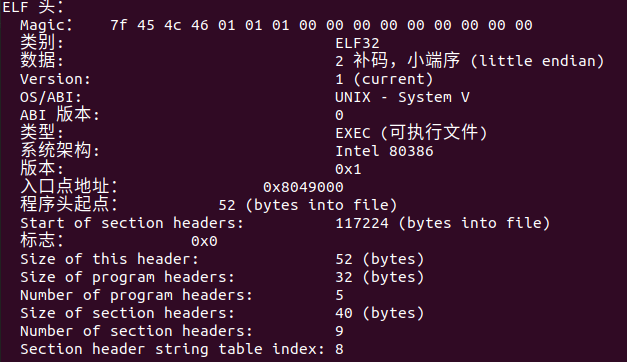
\includegraphics[scale=0.5]{fig/30.png}
\caption{system的ELF HEADER信息}
\label{fig:system's HEADER}
\end{figure}
可以看出,system程序入口点的地址是0x8049000,而不是在build.c中处理system模块时,认定的合法入口点地址0x0:
\begin{lstlisting}[breaklines]
	if (((long *) buf)[5] != 0)
		die("Non-GCC header of 'system'");
\end{lstlisting}
这是因为ld在将所有目标文件链接起来时,并不知道程序的入口点在哪里。实际的内核启动过程是从head.s中开始执行,因此给head.s的.globl中增加startup\_32,用于外部标识
\begin{lstlisting}[breaklines]
.text
.globl idt,gdt,pg_dir,startup_32
\end{lstlisting}
然后给 ./Makefile 中的ld加上选项 -e startup\_32 以指定入口点,同时添加 -Ttext 0 选项使startup\_32标号对应的地址为0x0
\begin{lstlisting}[breaklines]
LD	=ld -melf_i386 -e startup_32 -Ttext 0
\end{lstlisting}
同时,通过od命令:
\begin{lstlisting}[breaklines]
od -w4 -N 80 -x tools/system
0000000 457f 464c
0000004 0101 0001
0000010 0000 0000
*
0000020 0002 0003
0000024 0001 0000
0000030 9000 0804
\end{lstlisting}
可以看出,入口点地址0x08049000事实上位于ELF头中第28-30字节的位置上,也就是((long*)buf)[6]处,而不是build.c中原来的((long*)buf)[5]处,因此这里应修改为6。
\begin{lstlisting}[breaklines]
	if (((long *) buf)[6] != 0)
		die("Non-GCC header of 'system'");
\end{lstlisting}
\subsection{GCC\_HEADER的长度}	
通过使用readelf命令查看其ELF头信息,
\begin{figure}[htbp]
\centering
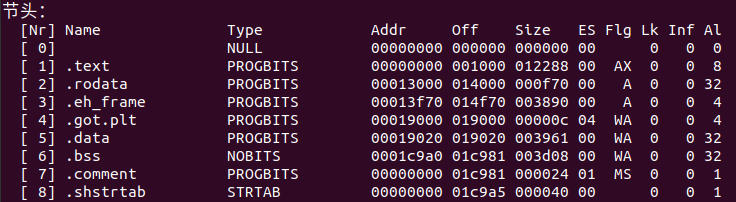
\includegraphics[scale=0.5]{fig/29.png}
\caption{GCC HEADER信息}
\label{fig:GCC HEADER}
\end{figure}
可以看出,.text的offset是从0x1000开始的(可能是由于GCC升级的原因?),因此需要将
\begin{lstlisting}[breaklines]
#define GCC_HEADER 1024
\end{lstlisting}
修改为:
\begin{lstlisting}[breaklines]
#define GCC_HEADER 4096
\end{lstlisting}
对应的main函数中的变量:
\begin{lstlisting}[breaklines]
	char buf[1024];
\end{lstlisting}
也需要修改为:
\begin{lstlisting}[breaklines]
	char buf[4096];
\end{lstlisting}
这样,一次把GCC\_HEADER全部读取,进行合法性检查后,就可以将剩余部分写入Image了。
\subsection{main函数}	
\begin{lstlisting}[breaklines]
int main(int argc, char ** argv)
{
	int i,c,id;
	char buf[4096];

	if (argc != 3)
		usage();
	for (i=0;i<sizeof buf; i++) buf[i]=0;
	if ((id=open(argv[1],O_RDONLY,0))<0)
		die("Unable to open 'boot'");
	if (read(id,buf,MINIX_HEADER) != MINIX_HEADER)
		die("Unable to read header of 'boot'");
	if (((long *) buf)[0]!=0x04100301)
		die("Non-Minix header of 'boot'");
	if (((long *) buf)[1]!=MINIX_HEADER)
		die("Non-Minix header of 'boot'");
	if (((long *) buf)[3]!=0)
		die("Illegal data segment in 'boot'");
	if (((long *) buf)[4]!=0)
		die("Illegal bss in 'boot'");
	if (((long *) buf)[5] != 0)
		die("Non-Minix header of 'boot'");
	if (((long *) buf)[7] != 0)
		die("Illegal symbol table in 'boot'");
	i=read(id,buf,sizeof buf);
	fprintf(stderr,"Boot sector %d bytes.\n",i);
	if (i>510)
		die("Boot block may not exceed 510 bytes");
	buf[510]=0x55;
	buf[511]=0xAA;
	i=write(1,buf,512);
	if (i!=512)
		die("Write call failed");
	close (id);
	
	if ((id=open(argv[2],O_RDONLY,0))<0)
		die("Unable to open 'system'");
	if (read(id,buf,GCC_HEADER) != GCC_HEADER)
		die("Unable to read header of 'system'");
	if (((long *) buf)[6] != 0)
		die("Non-GCC header of 'system'");
	for (i=0 ; (c=read(id,buf,sizeof buf))>0 ; i+=c )
		if (write(1,buf,c)!=c)
			die("Write call failed");
	close(id);
	fprintf(stderr,"System %d bytes.\n",i);
	return(0);
}
\end{lstlisting}
\part{include目录}
\section{asm子目录}
\subsection{system.h}	
\subsubsection{门操作符设置函数}	
\paragraph{\_set\_gate}	
门描述符有三种类型:任务门和中断门,陷井门,在门描述符中用不同的type区分。在\_set\_gate中默认所有的门处理函数的段选择子都是GDT的第一个段描述符。\\\\
\begin{figure}[htbp]
\centering
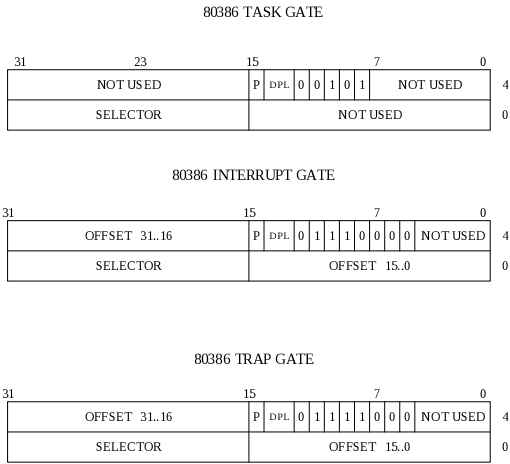
\includegraphics[scale=0.7]{fig/12.png}
\caption{门描述符结构}
\label{fig:Gate Discriptor}
\end{figure}
输入参数:\\
gate\_addr: 对应IDT表或者GDT/LDT表对应表项的位置\\
type: 门描述符的类型\\
dpl: 门描述符的特权等级\\
addr: 处理函数的地址\\
\begin{lstlisting}[breaklines]
#define _set_gate(gate_addr,type,dpl,addr) \
__asm__ ("movw %%dx,%%ax\n\t" \
	"movw %0,%%dx\n\t" \
	"movl %%eax,%1\n\t" \
	"movl %%edx,%2" \
	: \
	: "i" ((short) (0x8000+(dpl<<13)+(type<<8))), \
	"o" (*((char *) (gate_addr))), \
	"o" (*(4+(char *) (gate_addr))), \
	"d" ((char *) (addr)),"a" (0x00080000))
\end{lstlisting}
将\_set\_gate的宏定义展开可得
\begin{lstlisting}[breaklines]
movw dx, ax
movw %0, dx
movl eax,%1
movl edx,%2
\end{lstlisting}
其约束为:
\begin{list}{•}{•}
\item Output: 空
\item Input: 
\begin{enumerate}
\item "i" 允许立即整数操作数(具有常量值的操作数)。
\item "o" 允许使用内存操作数,但前提是该地址是可偏移的。
\item "d" \%edx, \%dx, \%dl
\item "a" \%eax, \%ax, \%al
\end{enumerate}
\item Clobber/Modify:省略。
\end{list}
对应的含义为
\begin{lstlisting}[breaklines]
	%0 = "i" = ((short) (0x8000+(dpl<<13)+(type<<8)))
	%1 = "o" = (*((char *) (gate_addr)))
	%2 = "o" = (*(4+(char *) (gate_addr)))
	"d": edx = ((char *) (addr))
	"a": eax = (0x00080000))
\end{lstlisting}
eax的初始值置为0x00080000,高位的0x0008(0b1000)对应中断处理程序的段选择符(1为索引,0表示GDT,RPL=00表示最高优先级);\\
edx的初始值置为addr,即offset;\\
第一条语句将addr的offset写到ax中,eax的内容即门描述符的低32位:选择子+offset低位;\\
第二条语句将((short) (0x8000+(dpl$<<$13)+(type$<<$8)))写到dx中,0x8=0b1000,即P=1,表示段存在标记;DPL=00,表示访问限制在内核态;type为14对应0xe,0b1110中断类型的门描述符,edx的内容即门描述符的高32位:offset的高位 + 门描述符的属性。\\
第三、四条语句将eax和edx中的内容写入门描述符所在的内存空间中去。
\paragraph{set\_intr\_gate}	
输入参数n和idt[n]表项对应;输入参数addr为对应中断处理函数的地址。\\
通过调用\_set\_gate函数,将idt[n]设置为中断类型的门描述符。\\
参数14为\_set\_gate函数的type,14对应0b1110,即中断类型的门描述符;\\
参数0为\_set\_gate函数的dpl,0对应内核优先级。
\begin{lstlisting}[breaklines]
#define set_intr_gate(n,addr) \
	_set_gate(&idt[n],14,0,addr)
\end{lstlisting}
\paragraph{set\_trap\_gate}	
输入参数n和idt[n]表项对应;输入参数addr为对应trap处理函数的地址。\\
通过调用\_set\_gate函数,将idt[n]设置为trap类型的门描述符。\\
参数15为\_set\_gate函数的type,15对应0b1111,即陷阱类型的门描述符;\\
参数0为\_set\_gate函数的dpl,0对应内核优先级。
\begin{lstlisting}[breaklines]
#define set_trap_gate(n,addr) \
	_set_gate(&idt[n],15,0,addr)
\end{lstlisting}
\paragraph{set\_system\_gate}	
输入参数n和idt[n]表项对应;输入参数addr为对应trap处理函数的地址。\\
通过调用\_set\_gate函数,将idt[n]设置为system类型的门描述符。\\
参数15为\_set\_gate函数的type,15对应0b1111,即陷阱类型的门描述符;\\
参数3为\_set\_gate函数的dpl,3对应普通优先级。
\begin{lstlisting}[breaklines]
#define set_system_gate(n,addr) \
	_set_gate(&idt[n],15,3,addr)
\end{lstlisting}
\subsubsection{TSS和LDT描述符设置函数}	
\begin{lstlisting}[breaklines]
#define _set_tssldt_desc(n,addr,type) \
__asm__ ("movw $104,%1\n\t" \
	"movw %%ax,%2\n\t" \
	"rorl $16,%%eax\n\t" \
	"movb %%al,%3\n\t" \
	"movb $" type ",%4\n\t" \
	"movb $0x00,%5\n\t" \
	"movb %%ah,%6\n\t" \
	"rorl $16,%%eax" \
	::"a" (addr), "m" (*(n)), "m" (*(n+2)), "m" (*(n+4)), \
	 "m" (*(n+5)), "m" (*(n+6)), "m" (*(n+7)) \
	)

#define set_tss_desc(n,addr) _set_tssldt_desc(((char *) (n)),addr,"0x89")
#define set_ldt_desc(n,addr) _set_tssldt_desc(((char *) (n)),addr,"0x82")
\end{lstlisting}
\paragraph{\_set\_tssldt\_desc}	
参数的含义:\\
\%1, n,Limit,段长低16bit,固定为104;\\
\%2, n+2,段基地址的低16bit,取自eax\\
\%3, n+4,段基地址的中8bit,取自eax\\
\%4, n+5,8bit;\\
p,p=1,表示段在内存中存在\\
dpl,dpl=00,表示内核特权级\\
s,s=0,表示系统段/门描述符\\
type,输入自type\\
\%5, n+6,8bit\\
g,g=0,表示长度单位为1字节\\
d,d=0,表示指令和数据是16位\\
x,未使用,填0\\
avl,保留,填0\\
段长高4位,固定填0\\
\%6, n+7,8bit,段基地址高8位,取自eax\\
\paragraph{\_set\_tss\_desc}	
type = 89,高位的8实际对应p,dpl,s bit,低位9=0b1001,0bit = 1,表示已访问,3bit=1,说明代码段,1bit=0,说明只执行,2bit=0,说明非一致代码段。
\paragraph{\_set\_ldt\_desc}	
type = 82,高位的8实际对应p,dpl,s bit,低位2=0b0011,0bit = 1,表示已访问,3bit=0,说明数据段,1bit=1,说明只读,2bit=0,说明向高位生长。

\subsection{io.h}
带延时操作的outb\_p和inb\_p,以及不带延时操作的outb和inb。
\subsubsection{outb}	
\begin{lstlisting}[breaklines]
#define outb(value,port) \
__asm__ ("outb %%al,%%dx"::"a" (value),"d" (port))
\end{lstlisting}
其中内联汇编参数含义:
\begin{list}{•}{•}
\item Output: 略
\item Input: “a”,表示al;(value)表示输出到变量value中;"d",表示dx;(port)表示dx置为port的值;
\item Clobber/Modify: 略
\end{list}
\subsubsection{inb}	
\begin{lstlisting}[breaklines]
#define inb(port) ({ \
unsigned char _v; \
__asm__ volatile ("inb %%dx,%%al":"=a" (_v):"d" (port)); \
_v; \
})
\end{lstlisting}
其中内联汇编参数含义:
\begin{list}{•}{•}
\item Output: “=a”,其中“=”表示只读,a表示al;(\_v)表示输出到变量\_v中;
\item Input: "d",表示dx;(port)表示dx置为port的值;
\item Clobber/Modify: 略
\end{list}
\subsubsection{outb\_p}	
\begin{lstlisting}[breaklines]
#define outb_p(value,port) \
__asm__ ("outb %%al,%%dx\n" \
		"\tjmp 1f\n" \
		"1:\tjmp 1f\n" \
		"1:"::"a" (value),"d" (port))
\end{lstlisting}
其中内联汇编参数含义:
\begin{list}{•}{•}
\item Output: 略;
\item Input: al=value, dx=port
\item Clobber/Modify: 略
\end{list}
在outb\_p中有两个标签“1”, 额外产生一条指令,用于等待端口操作。
\subsubsection{inb\_p}	
\begin{lstlisting}[breaklines]
#define inb_p(port) ({ \
unsigned char _v; \
__asm__ volatile ("inb %%dx,%%al\n" \
	"\tjmp 1f\n" \
	"1:\tjmp 1f\n" \
	"1:":"=a" (_v):"d" (port)); \
_v; \
})
\end{lstlisting}
\begin{list}{•}{•}
\item Output: \_v=a 
\item Input: dx=port
\item Clobber/Modify: 略
\end{list}
在inb\_p中有两个标签“1”, 额外产生一条指令,用于等待端口操作。
\section{linux子目录}
\subsection{sched.h}	
\begin{lstlisting}[breaklines]
struct tss_struct {
	long	back_link;	/* 16 high bits zero */
	long	esp0;
	long	ss0;		/* 16 high bits zero */
	long	esp1;
	long	ss1;		/* 16 high bits zero */
	long	esp2;
	long	ss2;		/* 16 high bits zero */
	long	cr3;
	long	eip;
	long	eflags;
	long	eax,ecx,edx,ebx;
	long	esp;
	long	ebp;
	long	esi;
	long	edi;
	long	es;		/* 16 high bits zero */
	long	cs;		/* 16 high bits zero */
	long	ss;		/* 16 high bits zero */
	long	ds;		/* 16 high bits zero */
	long	fs;		/* 16 high bits zero */
	long	gs;		/* 16 high bits zero */
	long	ldt;		/* 16 high bits zero */
	long	trace_bitmap;	/* bits: trace 0, bitmap 16-31 */
	struct i387_struct i387;
};

struct task_struct {
/* these are hardcoded - don't touch */
	long state;	/* -1 unrunnable, 0 runnable, >0 stopped */
	long counter;
	long priority;
	long signal;
	fn_ptr sig_restorer;
	fn_ptr sig_fn[32];
/* various fields */
	int exit_code;
	unsigned long end_code,end_data,brk,start_stack;
	long pid,father,pgrp,session,leader;
	unsigned short uid,euid,suid;
	unsigned short gid,egid,sgid;
	long alarm;
	long utime,stime,cutime,cstime,start_time;
	unsigned short used_math;
/* file system info */
	int tty;		/* -1 if no tty, so it must be signed */
	unsigned short umask;
	struct m_inode * pwd;
	struct m_inode * root;
	unsigned long close_on_exec;
	struct file * filp[NR_OPEN];
/* ldt for this task 0 - zero 1 - cs 2 - ds&ss */
	struct desc_struct ldt[3];
/* tss for this task */
	struct tss_struct tss;
};

\end{lstlisting}
\subsection{sys.h}	
\subsubsection{sys\_call\_table[]}	
\begin{lstlisting}[breaklines]
fn_ptr sys_call_table[] = { sys_setup, sys_exit, sys_fork, sys_read,
sys_write, sys_open, sys_close, sys_waitpid, sys_creat, sys_link,
sys_unlink, sys_execve, sys_chdir, sys_time, sys_mknod, sys_chmod,
sys_chown, sys_break, sys_stat, sys_lseek, sys_getpid, sys_mount,
sys_umount, sys_setuid, sys_getuid, sys_stime, sys_ptrace, sys_alarm,
sys_fstat, sys_pause, sys_utime, sys_stty, sys_gtty, sys_access,
sys_nice, sys_ftime, sys_sync, sys_kill, sys_rename, sys_mkdir,
sys_rmdir, sys_dup, sys_pipe, sys_times, sys_prof, sys_brk, sys_setgid,
sys_getgid, sys_signal, sys_geteuid, sys_getegid, sys_acct, sys_phys,
sys_lock, sys_ioctl, sys_fcntl, sys_mpx, sys_setpgid, sys_ulimit,
sys_uname, sys_umask, sys_chroot, sys_ustat, sys_dup2, sys_getppid,
sys_getpgrp,sys_setsid};
\end{lstlisting}
\part{CPU的构造}
\section{8086}
\subsection{8086概述}
Intel8086拥有四个16位的通用寄存器,也能够当作八个8位寄存器来存取,以及四个16位索引寄存器(包含了堆栈指标)。资料寄存器通常由指令隐含地使用,针对暂存值需要复杂的寄存器配置。它提供64K8位元的输出输入(或32K16位元),以及固定的向量中断。大部分的指令只能够存取一个内存位址,所以其中一个操作数必须是一个寄存器。运算结果会储存在操作数中的一个寄存器。\\\\
Intel8086有四个内存区段(segment)寄存器,可以从索引寄存器来设定。区段寄存器可以让CPU利用特殊的方式存取1MB内存。8086把段地址左移4位然后把它加上偏移地址。大部分的人都认为这是一个很不好的设计,因为这样的结果是会让各分段有重叠。尽管这样对组合语言而言大部分被接受(也甚至有用),可以完全地控制分段,使在编程中使用指针(如C编程语言)变得困难。它导致指针的高效率表示变得困难,且有可能产生两个指向同一个地方的指针拥有不同的地址。更坏的是,这种方式产生要让内存扩充到大于1MB的困难。而8086的寻址方式改变让内存扩充较有效率。\\\\
8086处理器的时钟频率介于4.77MHz(在原先的IBMPC频率)和10MHz之间。8086没有包含浮点指令部分(FPU),但是可以通过外接数学辅助处理器来增强浮点计算能力。Intel8087是标准版本。\\\\
\subsection{8086引脚及功能}
\begin{figure}[htbp]
\centering
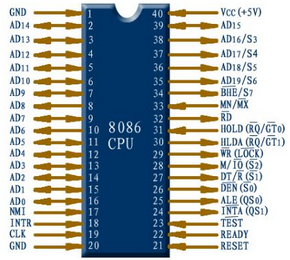
\includegraphics[scale=0.7]{fig/13.png}
\caption{8086引脚图}
\label{fig:Intel CPU 8086}
\end{figure}

⑴AD15~AD0(addressdatabus):地址/数据总线,双向,三态。\\
这是一组采用分时的方法传送地址或数据的复用引脚。根据不同时钟周期的要求,决定当前是传送要访问的存储单元或I/O端口的低16位地址,还是传送16位数据,或是处于高阻状态。\\\\
⑵A19/S6~A16/S3(address/status):地址/状态信号,输出,三态。\\
这是采用分时的方法传送地址或状态的复用引脚。其中A19~A16为20位地址总线的高4位地址,S6~S3是状态信号。S6表示CPU与总线连接的情况,S5指示当前中断允许标志IF的状态。S4,S3的代码组合用来指明当前正在使用的段寄存器。S4,S3的代码组合及对应段寄存器的情况。\\\\
⑶BHE(低)/S7(bushighenable/status):允许总线高8位数据传送/状态信号,输出,三态。\\
为总线高8位数据允许信号,当低电平有效时,表明在高8位数据总线D15~D8上传送1个字节的数据。S7为设备的状态信号。\\\\
⑷RD/(read):读信号,输出,三态,低电平有效。\\
信号低电平有效时,表示CPU正在进行读存储器或读I/O端口的操作。\\\\
⑸READY(ready):准备就绪信号,输入,高电平有效。\\
READY信号用来实现CPU与存储器或I/O端口之间的时序匹配。当READY信号高电平有效时,表示CPU要访问的存储器或I/O端口已经作好了输入/输出数据的准备工作,CPU可以进行读/写操作。当READY信号为低电平时,则表示存储器或I/O端口还未准备就绪,CPU需要插入若干个“TW状态”进行等待。\\\\
⑹INTR(interruptrequest):可屏蔽中断请求信号,输入,高电平有效。\\
8086CPU在每条指令执行到最后一个时钟周期时,都要检测INTR引脚信号。INTR为高电平时,表明有I/O设备向CPU申请中断,若IF=1,CPU则会响应中断,停止当前的操作,为申请中断的I/O设备服务。\\\\
⑺TEST/(test):等待测试控制信号,输入,低电平有效。\\
信号用来支持构成多处理器系统,实现8086CPU与协处理器之间同步协调的功能,只有当CPU执行WAIT指令时才使用。\\\\
⑻NMI(non-maskableinterrupt):非屏蔽中断请求信号,输入,高电平有效。\\
当NMI引脚上有一个上升沿有效的触发信号时,表明CPU内部或I/O设备提出了非屏蔽的中断请求,CPU会在结束当前所执行的指令后,立即响应中断请求。\\\\
⑼RESET(reset):复位信号,输入,高电平有效。\\
RESET信号有效时,CPU立即结束现行操作,处于复位状态,初始化所有的内部寄存器。复位后各内部寄存器的状态,当RESET信号由高电平变为低电平时,CPU从FFFF0H地址开始重新启动执行程序。\\\\
⑽CLK(clock):时钟信号,输入。\\
CLK为CPU提供基本的定时脉冲信号。8086CPU一般使用时钟发生器8284A来产生时钟信号,时钟频率为5MHz~8MHz,占空比为1:3。\\
⑾VCC电源输入引脚。\\
8086CPU采用单一+5V电源供电。\\\\
⑿GND:接地引脚。\\\\
⒀MN/MX/(minimum/maximum):最小/最大模式输入控制信号。\\
引脚用来设置8086CPU的工作模式。当为高电平(接+5V)时,CPU工作在最小模式;当为低电平(接地)时,CPU工作在最大模式。
\subsection{8086工作模式}
\paragraph{最小模式}
由8086单一微处理器构成的小系统。在这种方式下,由8086 CPU直接产生小系统所需要的全部控制信号。器系统特点是:总线控制逻辑直接由8086 CPU产生和控制。若有CPU以外的其他模块想占用总线,则可以向CPU提出请求,在CPU允许并响应的情况下,该模块才可以获得总线控制权,使用完后,又将总线控制权还给CPU。
\paragraph{最大模式}
用于实现多处理机系统,其中,8086CPU被称为主处理器,其他处理器被称为协处理器。在这种方式下,8086CPU不直接提供用于存储器或I/O读写的读写命令等控制信号,而是将当前要执行的传送操作类型编码为3个状态位输出,由总线控制器8288对状态信号进行译码产生相应控制信号。最大模式系统的特点是:总线控制逻辑由总线控制器8288产生和控制,即8288将主处理器的状态和信号转换成系统总线命令和控制信号。协处理器只是协助主处理器完成某些辅助工作,即被动的接受并执行来自主处理器的命令。和8086配套使用的协处理器有两个:一个是专用于数值计算的协处理器8087,另一个是专用于输入输出操作的协处理器8089。8087通过硬件实现高精度整数浮点数运算。8089有其自身的一套专门用于输入输出操作的命令系统,还可带局部存储器,可以直接为输入输出设备服务。增加协处理器,使得浮点运算和输入输出操作不再占用8086时间,从而大大提高了系统的运行效率。

\subsection{8086系统组成}
8086是一种微处理器,再加上必须的支持芯片,如时钟发生器,地址锁存器,总线驱动器,存储器和I/O接口等,才能构成一台完整的微型计算机。根据外部设备的数量和系统复杂程度,8086可以选用两种系统构成模式,最小模式和最大模式。最小模式是单CPU系统,在这种系统中,8086的MN/MX引脚接高电平,系统全部的控制信号都直接由CPU提供。最大模式是多CPU系统,此时MN/MX引脚接低电平,必须通过8288总线控制器对CPU的状态信息进行译码才能产生系统必须的控制信号。
\paragraph{地址锁存}
8086的AD15~~AD0是地址/数据复用线,即CPU与存储器进行信息交换时,首先在T1状态,先由CPU送出访问存储单元的地址信息到AD15~~AD0上,随后又用这些线来传送数据。所以在数据送上总线以前,必须先将地址锁存起来。可用8282或74LS373锁存8086的单向地址AD15~~AD0. 可以使用三片8282,这是因为8282只具有8位锁存功能,而8086具有20位地址和一根BHE信号。若系统存储器容量较小,使用不到20位地址信息,也可只用2片8282。
\paragraph{双向数据总线驱动器}
CPU可以直接将数据发送到数据总线上。而无需锁存。为了增加总线负载能力,CPU数据总线一般要加上驱动器,且要求双向驱动器,一般采用8位双向驱动器8286或74LS245.由于8086数据总线是16位的,所以要用2片8286.8286的Ai引脚接CPU的ADi,其Di引脚接到系统数据总线D1上,并将8086的DT/R接8286的T引脚,当DT/R为高电平時,数据从CPU发送到数据总线上.DT/R为低电平時,CPU从数据总线上接收数据.8286的OE脚接8086的DEN脚。当8086的DEN为低电平时,才允许数据输入或输出。
\paragraph{时钟发生器/驱动器}
8086所需时钟脉冲CLK由8284提供.8284输出时钟CLK的频率,取决X1,X2跨接石英晶体的频率。除此以外,8284还向8086提供定时和宽度符合要求的RESET复位信号及符合要求的READY信号。
\paragraph{存储器部件}
8086能直接寻址1MB存储空间。这个存储空间分为两个512KB存储体。一个存储體由奇地址单元组成,用于存储16数据的高字节,另一个存储体由偶地址单元组成,用于存储16位数据低字节。前者称为奇地址存储器,后者称为偶地址存储体。偶地址存储体的8位数据总线接CPU的数据总线D7~~D0,而奇地址存储体8位数据线接数据总线D15~~D8.地址线A19~~A1同时接到两个存储体,而A0作为偶地址选中信号即A0=0时,选中偶存储体.BHE作为奇地址片选信号,BHE=0时选中奇存储体。所以两个存储体可以同时读出或写入,也可单独选中一个存储体。
\paragraph{I/O端口}
一个完整的微机系统必须有I/O设备.I/O设备都有端口地址号.CPU通过地址总线发出端口地址,经过端口地址译码器输出,送到端口的片选引脚而选定指定的端口.8086根据执行命令是访问存储器指令还是输入输出指令,来使M/IO控制信号是高电平或是低电平,以区分地址总线上的地址是访问存储器还是访问外设.

\subsection{8086的内存管理}
8086CPU有20位地址线,那么它能寻址的范围$2^{20}$B = 1048576B = 1024KB = 1MB。但是在CPU内部的总线和寄存器都是十六位的,用它们做地址寄存器只能寻址64KB单元,它是如何管理1M的空间的呢?秘密在BIU区域存在一个地址加法器,地址线经过这个加法器之后从16位变成了20位。那么这个过程是如何实现的呢?\\\\
秘密是采用分段技术,将1MB的内存空间分成若干段,每一段的第一个地址称为段首址,并且用段首址来表示这一段的内存地址。段首址必须要能被16整除,这样的话,段首址就可以用16位来保存,低4位全部为零,高16位可放在段寄存器中。\\\\
段首址保存在段寄存器来表示,包括CS(代码段)、DS(数据段)、SS(堆栈段)和ES(附加段);偏移地址用 IP 来表示。 \\
逻辑地址:包括段首址和偏移地址,如CS:IP。\\
物理地址:实际的内存地址,用20bit表示。\\\\
那么逻辑地址是如何变成物理地址呢?公式如下:\\
物理地址 = 段首址 * 0x10 + 段内偏移量\\\\
举个例子:如果一个内存地址(物理地址)为:2304AH,段首址为2304H。那么逻辑地址为:2304H:000AH。\\\\
地址加法器就是进行这样一个运算,让16的CPU可以寻址1MB的内存空间。

%https://www.cnblogs.com/yilang/p/11321458.html
\section{80286}
\subsection{80286概述}
INTEL 1982年推出80286芯片,该芯片相比8086和8088有了飞跃式发展,虽然它仍是16位结构,但在CPU内部含有13.4万个晶体管,时钟频率由最初6MHz逐步提高到20MHz。内部和外部数据总线皆为16位,地址总线24位,可寻址内存大小达到16Mb。80286兼容了8086所有功能,并且是8086的向上兼容的微处理器,使8086的汇编语言程序可以不做任何修改地在80286上运行。同时80286的推出也是实模式和保护模式CPU的分水岭。80286微处理器内部有4个功能部件,即地址部件AU,指令部件IU,执行部件EU和总线部件BU。这四个部件的并行操作,提高了吞吐率,加快了处理速度。\\\\
\subsection{80286引脚及功能}
\begin{figure}[htbp]
\centering
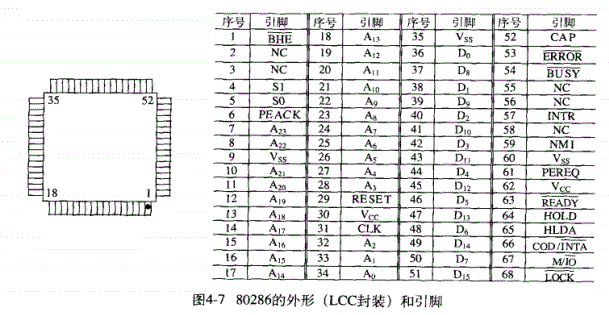
\includegraphics[scale=0.6]{fig/14.png}
\caption{80286引脚图}
\label{fig:Intel CPU 80286}
\end{figure}
80286具有68条外部引脚,可封装成PGA或LCC两种形式,它的多数引脚与8086相同,对此不在重复,下面介绍那些功能不同的引脚:\\\\
A0~A23-----24位地址\\\\
D0~D15-----16位数据线\\\\
S1、S0 --系统状态输出;\\\\
COD/INTA 代码或中断响应,输出;\\\\
M/IO  选择存储器或I/O端口\\\\
PEREQ 协处理器操作请求\\\\
PEACK 协处理器操作响应\\\\
BUSY  协处理器忙 \\\\ 
ERROR 协处理器出错\\\\
CAP 滤波电容输入\\\\
VSS  系统的参考地\\\\
NC  内部没有连接
\subsection{80286结构}
8086内部由执行单元和总线接口单元两大部分组成。而80286恰好与此不同,它由总线单元、指令单元、执行单元及地址单元四大部分组成,这些打印可以同步地并行工作,实现流水线作业,避免传统的顺序处理方式,最大限度的发挥处理器性能。
\begin{figure}[htbp]
\centering
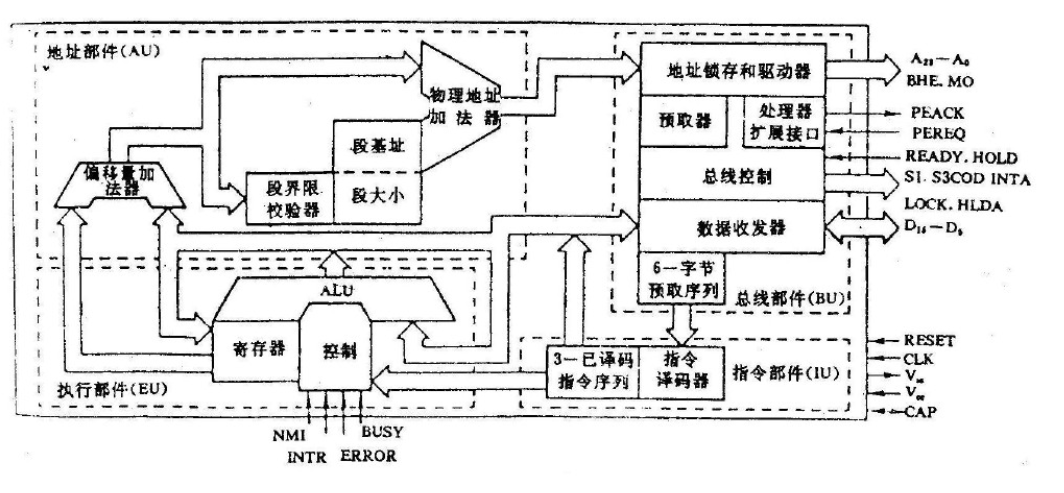
\includegraphics[scale=0.35]{fig/15.png}
\caption{80286结构图}
\label{fig:80286 component}
\end{figure}
\paragraph{地址单元}
Adress Unit, AU 由地址偏移量加法器,段基址寄存器,段容量寄存器,段限检查器和物理地址加法器等组成。同是还增加了对方式操作时的存储器管理和保护机构。地址部件的职责是根据执行部件EU的请求,从EU的寄存器中取出寻址信息,根据寻址规则形成物理址,然后把物理地址送到总线部件BU的地址锁存器和驱动器中,所长生的地址是物理存储器地址或I/O设备的端口。在地址单元中,由偏移量加法器进行有效偏移地址计算时,要对其偏移量的段界限进行检查,并且还要对段存取检查,最后才进行从虚拟地址到物理地址的转换。
\paragraph{总线单元}
总线单元(Bus Unit, BU)由地址存储器和驱动器、总线控制、数据收发器、预取器和指令预取队列以及协处理器借口等组成,他是由CPU与系统之间的一个高速接口,其任务是使CPU以最高速率从外部取代码和读/写数据。总线单元生成存储器及IO请求所必须的地址、数据、指令信号,并执行CPU的所有总线操作。
\paragraph{指令单元}
指令单元(Instruction Unit, IU)由指令译码器和已被译码的指令队列组成,其功能是不断的从总线部件BU的预取代码队列中取出指令,译码后放倒已被译码的指令队列中,为执行部件EU执行指令做好准备。IU的引入进一步改善了流水操作,IU内部始终存放着3条已译码的指令,执行部件EU执行的就是这些已经译码指令。IU和EU的并行操作,缩短了执行指令的时间。
\paragraph{执行单元}
执行单元(Execution Unit, EU)由算术逻辑部件ALU,控制器和微代码只读存储器构成,EU负责执行指令,所执行的指令时从IU中所取来的已译码的指令。
\subsection{80286工作模式}
\paragraph{实地址模式}
系统开机CPU复位时,自动进入实地址模式,A23~A20自动置为0,以 A19~A0寻址1M的存储空间。也就是8086工作模式。
\paragraph{虚地址保护模式}
当机器状态字MSW的PE位置1时,进入保护模式。该模式主要针对在多任务机制中的存储管理。其有两个方面的含义:\\\\
虚地址 —— 应用程序可以寻址一个比实际物理地址空间(16M)大得多的虚存空间(1024M)。\\
保护 —— 对存储空间的(数据和程序的)保护,保障多任务机制。\\\\
保护模式下的寻址过程:为实现“虚地址”和“保护”两大功能,系统必须提供一种“机制”或“平台”或一个“中间环节”来实施并完成上述两大功能。而这个所谓“中间平台”的核心部分,就是传说中的描述子 (Descriptor)。
描述子的作用:刻划存储段的属性(比如一个段的保护属性)并提供虚地址到实地址转化的信息。描述子的引入,使存储器的构成就由单一的存储段,转变成了若干存储段和若干存储段的描述子构成,因此存储器的组织形式就由实地址模式的单一的“存储段”变为两级结构,即:(1)一系列可变长的段(1 ~ 64K)、(2) 一系列的描述子。而对内存进行访问时,那几个段寄存器存放的再不是段基址了,而是一种用来定位段描述子的东西,叫做选择子。由选择子找到对应的段,再加上偏移量,得到最终的物理地址(从 ① 到 ④ )。
\begin{figure}[htbp]
\centering
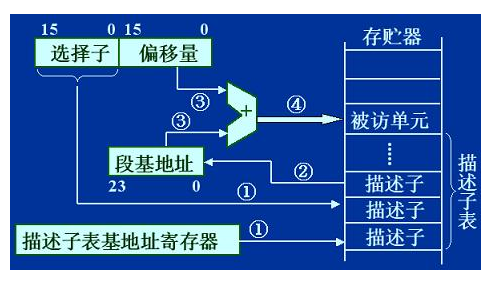
\includegraphics[scale=0.7]{fig/16.png}
\caption{80286虚地址寻址}
\label{fig:80286 virtual memory}
\end{figure}
\paragraph{数据/代码段描述子}
描述子是一个位于内存的数据结构, 用于描述所对应的(或所描述的)那个存储段的访问属性。 这些属性包括:一个存储段可以被哪一特权级的任务访问、该段的大小、该段的读写/可执行权限、该段的基地址。\\\\
\begin{figure}[htbp]
\centering
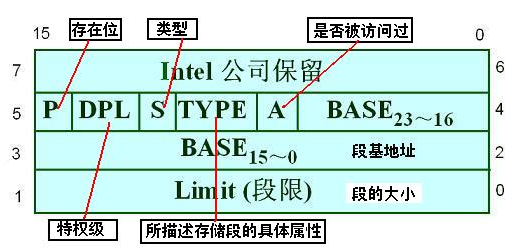
\includegraphics[scale=0.7]{fig/17.png}
\caption{80286数据/代码段描述符}
\label{fig:80286 Segment Discriptor}
\end{figure}
BASE23~16 BASE15~0 : 描述子所描述的那个段的段基地址。\\
Limit (段限): 该段的最后一个字节的偏移量,指明了该段的大小。\\
A: 该段是否被访问,该段已被访问过,则 A←1;该段未被访问过,则 A←0。该位与操作系统的时钟相结合,可进行段淘汰算法。\\
S: 描述子类型,1 代表数据代码段描述子;0 代表系统描述子(如门描述子/任务状态段描述子)\\
DPL: 共两位,规定可以访问该描述子所描述的那个段的任务的最低特权级。\\
P: 0 表示该描述子所描述的段不在物理空间;1 表示该描述子所描述的段在物理空间。\\
TYPE:由三位构成,即数据段(E, ED, W) 或代码段(E, C, R)。这个TYPE对所描述的存储段的具体属性有着极其重要的意义。\\
若该段为数据段,则 E=0,需要配合TYPE的ED和W。ED为0则段向上生长,所以要求偏移量小于Limit(段限);ED为1则段向下生长,所以要求偏移量大于Limit(段限);W为0则该数据段只能读,不能写;如果W为1则该数据段可读、可写。\\
若该段为代码段,则E=1,需要配合TYPE的C和R(ED变成了C,W变成了R)。C为0则非一致性代码段访问和被访问代码段特权级相同;C为1则一致性代码段访问和被访问代码段特权级可以不同;R为0则代码段只能执行,不能读;R为1代码段可以执行,也可以读。
\paragraph{选择子}
选择子主要扮演以下三个角色:\\\\
◆ 指明使用该选择子的任务的特权级\\
◆ 指明所要访问的描述子在描述子表中的偏移量(索引)\\
◆ 指明访问全局描述子表还是访问局部描述子\\\\
\begin{figure}[htbp]
\centering
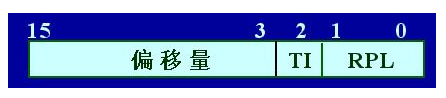
\includegraphics[scale=0.7]{fig/18.png}
\caption{80286 选择子}
\label{fig:80286 Segment Selector}
\end{figure}
RPL: 请求特权级,用以表示使用该选择子的任务的特权级。当前运行任务的特权级称为当前特权级CPL。一般有: RPL= CPL\\
TI: 区分访问全局描述子还是局部描述子:TI为0——访问全局描述子;TI为1——访问局部描述子。\\
偏移量D15~D3:所要访问的描述子在描述子表中的偏移量。
\paragraph{门描述子}
门描述子也是描述子的一种,但它并不用于描述某个存储段的属性,而是控制同一个任务内不同代码段之间的转移,或用于控制任务之间的切换。门描述子有四种类型:调用门、中断门、自陷门、任务门。前三者是控制同一个任务内不同代码段之间的转移,定义在IDT表中;后一个是控制任务之间的切换,可在LDT、GDT和IDT任何一个表中,如果将任务门放在IDT表中, 即可以通过访问IDT表来访问任务门, 则可以达到由于中断而发生任务切换的目的。
\begin{itemize}
\item 调用门 → 主程序调用子程序、转移指令
\item 中断门 → 中断引起的代码段转移
\item 自陷门 → 自陷引起的代码段转移。与中断门区别仅在于调用中断门时要将IF置0, 调用自陷门则不管IF标志。
\end{itemize}
中断/自陷/调用门的使用场合:在保护模式下, 同一任务的不同代码段, 也有不同的特权级, 意味着主调代码段与被调代码段可能处于不同的特权级, 因此需要指明目标代码段特权级, 并由此实现这同一任务的特权级的改变。为实现特权级的改变, 通过 “门”这样一个描述子中提供目标代码段描述子的选择子, 该选择子的低2位(RPL)指明目标代码段的特权级。
\begin{itemize}
\item 同级特权级之间转移:可以使用也可以不使用“门”。不使用意味着在指令中直接引用目标代码段描述子的选择子。
\item 向更低特权级转移:可以使用也可以不使用调用门, 但不管使用与否, 都只能发生在RET或IRET两种情况。可以直接引用目标代码段描述子的选择子, 此时,该选择子中的RPL将成为新的CPL2。
\item 向更高级转移:向更高特权级转移, 必须“门”来实现。举个例子,假设:源代码段的特权级为CPL1;目标代码段的特权级为CPL2;
\end{itemize}
\begin{figure}[htbp]
\centering
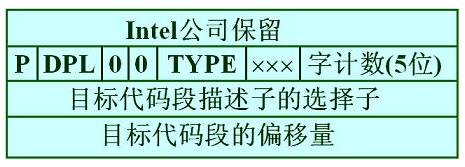
\includegraphics[scale=0.7]{fig/20.png}
\caption{80286门描述符}
\label{fig:80286 Gate Discriptor}
\end{figure}
门描述子的格式如下:
\begin{itemize}
\item P: 1位,0表示该描述子内容无效;1表示该描述子内容有效;
\item DPL:2位,规定可以访问该描述子所描述的那个段的任务的最低特权级;
\item TYPE: 3位,为4(0b100)表示调用门、为5(0b101)表示任务门、为6(0b110)表示中断、为7(0b111)表示自陷门;
\item 字计数:5位,仅调用门使用;
\item 目标代码段描述子的选择子:16位;若是任务门,则表示TSS描述子的选择子;
\item 目标代码段偏移量:16位;对任务门无效。
\end{itemize}
通过描述符中的DPL设定,“门”为目标代码段提供了保护,如果不允许低优先级的代码来访问,可以把“门”给关闭。
\paragraph{任务状态段描述子}
任务状态段(Task State Segment 简称TSS)是用于存放在任务被切换时刻的处理器现场的一个存储段。注意,它是一个段,跟代码段,数据段一样,而且每个任务都有一个TSS。TSS中的内容随着任务的执行不断发生变化。 TSS的内容主要包括:该任务断点各寄存器的内容,指向该任务的LDT选择子, 任务在特权级0、1、2的堆栈指针以及指向前一个任务的TSS的选择子等。
\paragraph{任务切换方式}
直接切换 —— 直接引用目标任务状态段描述子的选择子\\
同特权级之间或向更低的特权级切换, 可采用直接切换。直接切换方式不使用任务门,直接引用任务状态段描述子的选择子来访问TSS,以实现任务切换。\\
间接切换 —— 从引用任务门开始, 由任务门提供目标任务状态段描述子的选择子。间接切换则可以向任何特权级切换。需要使用任务门。
\paragraph{任务切换的引起}
任务切换可由JMP、CALL指令或中断(INT)指令,异常或外部中断引起。JMP、CALL指令可以直接引用一个任务状态段, 也可以先引用一个GDT或LDT中的任务门, 再由任务门的目标选择子引用任务状态段而实现任务转换。中断类的指令则必须先从IDT中引用任务门,再由任务门的目标选择子引用状态任务段而实现任务转换。IRET指令通过引用IDT中的任务门而返回到原任务中去。
\subsection{80286内存管理}
\paragraph{虚存空间的计算} 80286有两种工作模式,在实模式下,跟8086内存管理一样,只能管理和寻址1MB物理内存。而在保护模式下,不仅可以管理$2^{24}=16$MB物理内存,而且最多可访问1GB的虚拟空间:描述子数量 * 描述子对应的段长。
\begin{enumerate}
\item 段的度对应段描述符中16位的limit,对应最大值$2^{16}$ = 64K;\\
\item 段的数量对应可有选择子访问到的描述子的数量,选择子偏移量13bit,可以访问的描述子的数量为$2^{13}$ = 8K (个描述子)\\
\item 选择子的TI位区分了全局描述子或局部描述子,可访问的描述子的总数为全局描述子或局部描述子之和:8K + 8K = 16K
\end{enumerate}
因此,可访问的虚地址空间为: 16K × 64K = 1000M = 1G \\\\
\begin{figure}[htbp]
\centering
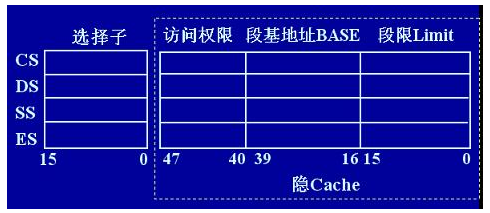
\includegraphics[scale=0.7]{fig/19.png}
\caption{80286 段寄存器和隐Cache}
\label{fig:80286 Segment Registor and Cache}
\end{figure}
在保护模式下访存时,首先需要访问选择子,再得到描述子。为了加快访问速度,从80286开始,每个段寄存器都配备了一个高速缓冲寄存器,称之为段描述子高速缓冲寄存器(隐Cache)。当将一个选择子装入某个段寄存器时,处理器将自动从描述子表中取出相应的描述子,将描述子的信息保存到对应高速缓冲寄存器中。 以后对该段进行访问时,处理器都使用对应高速缓冲寄存器中的描述子信息,从而不再从描述子表中取描述子。隐Cache位于CPU内部,其内容随着段寄存器的修改而被重新装入,这种装入操作对程序员透明。\\\\
假设一个32位的虚地址:005E0100H,其中选择子为005EH, 低3位为0b110, 其中TI=1,访问局部描述子表(LDT); RPL=2(10);由于每个描述子为8个字节, 则选择子中的偏移量*8即为所对应描述子(偏移8个字节);也即将选择子低3位置为0, 0058H即为描述子相对LDT基地址的偏移。虚地址的偏移量为0100H。
我们假设 LDTR=100000H\\\\
第一步:将描述子表基地址LDTR+选择子偏移量 = 100000H + 0058H = 100058H\\
第二步:由物理地址100058H访问并得到相应的描述子,检查对该描述子访问的合法性(比较CPL和DPL),假设DPL=3, 则CPL=RPL=2≤DPL(数值上),访问是合法的。\\
第三步:由描述子中的TYPE,若为数据段,将虚地址中的偏移量(即0100H)与描述子中的段限Limit进行比较,以确定访问是否越界,假设描述子中给出的段基地址为046000H, Limit=2000H, 有偏移量0100≤段限2000H,未越界。\\
第四步:形成物理地址046000+0100=046100H(24位),以此访问存储单元的物理地址,得到所需要的数据。
%https://www.cnblogs.com/yilang/p/11322645.html
\section{80386}
\subsection{80386概述}
80386处理器被广泛应用在1980年代中期到1990年代中期的IBM PC相容机中。这些PC机称为「80386电脑」或「386电脑」,有时也简称「80386」或「386」。80386的广泛应用,将PC机从16位时代带入了32位时代。80386的强大运算能力也使PC机的应用领域得到巨大扩展,商业办公、科学计算、工程设计、多媒体处理等应用得到迅速发展。它的数据总线和地址总线都是32位,直接寻址的内存空间4GB,虚拟地址空间为64TB。芯片上集成了27.5万个晶体管,主频16-33MHz。它是X86第一个真正的32位CPU,它能提供真正的多任务处理和建立虚拟系统的能力。
\subsection{80386的引脚及功能}
\begin{figure}[htbp]
\centering
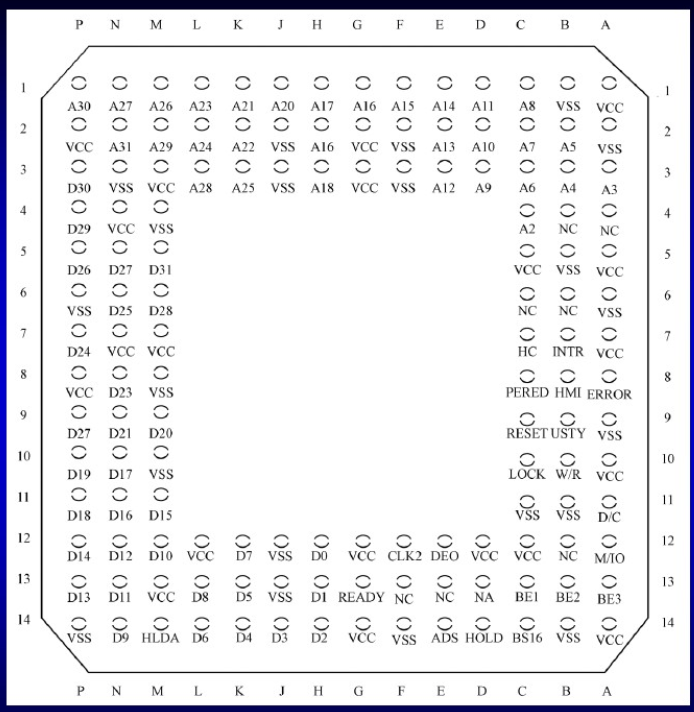
\includegraphics[scale=0.4]{fig/21.png}
\caption{80386引脚图}
\label{fig:Intel CPU 80386}
\end{figure}
80386 DX有132根引脚,采用PGA(Pin Grid Array,引脚网格阵列)封装,采用这种封装工艺单根引脚所占用的面积较双列直插时小,因此引脚数目可以多一些,不必再采用引脚复用技术。因此,在80386中数据线和地址线是分开设置的,控制信号和状态信号也不再复用引脚。其中34 条地址线(A31~A2、BE3~BE0),32 条数据线(D31~D0),3 条中断线,1条时钟线,13 条控制线,20 条电源线VCC,21条地线VSS,还有8 条为空。\\\\
与8086/8088 相比,需要说明以下几点:\\
1)时钟( CLK2): 80386 的基本定时信号由CLK2 提供。CLK2 的频率是80386 内部时钟信号频率的两倍,输入该信号与82384 时钟信号同步,经80386 内部2 分频之后得到80386 的工作基准频率信号。\\
2)数据总线(D31~D0):为80386 和其他设备之间提供数据通路,32 位数据总线,双向三态,一次可传送8 位、16 位或32 位数据,由输入信号(BE3~BE0)和BE16确定。在任何写操作周期(包括暂停周期和停机周期),80386 总是驱动数据总线的所有32 位信号,而不管当前总线的实际宽度。\\
3)地址总线(A31~A2,BE3~BE0) 。\\
A31~A2:地址总线,输出三态,和BE3~BE0相结合起到32位地址的作用。80386地址总线包含A2~A31地址线和字节选通线BE3~BE0。BE3~BE0线的功能与8086和80286系统的A0和BHE非常相似,它们是内部地址信号A0和A1的译码。由于80386有一个32位数据总线,所以内存可以建立4B宽的存储体。BE3~BE0信号是用来选通这4B个存储体。这些单独选通可以使80386 的内存传送或者接收字节、字或者双字。\\
BE3~BE0:字节选通信号。用于选通在当前的传送操作要涉及4B数据中的哪几个字节。BE0对应于D0~D7,BE1对应于D8~D15,BE2对应于D16~D23,BE3对应于D24~D31。\\
4)总线周期定义信号(M/IO,W/R,D/C,LOCK,三态,输出,用来定义正在进行的总线周期类型)。\\
M/IO:存储器/输入输出选择信号,输出信号。高电平时访问存储器,低电平时访问I/O 端口。80386 直接I/O 端口简单地把8086 和80286 端口结构扩充成32 位端口。32 位I/O 端口可以通过并联8 位I/O 端口设备(如8255A)来构成。80386 可以使用所有8 位端口地址的IN 或OUT 指令来编址256 个8 位端口、128 个16 位端口、64 个32 位端口。使用DX 寄存器存放16 位端口地址,80386 可以编址64K 个8 位端口、32K 个16 位端口或8K 个32 位端口。\\
W/R:读/写控制输出信号,高电平时写入,低电平时读出。\\
D/C:数据/指令控制信号,输出。高电平时传送数据,低电平时传送指令代码,D/C指示总线操作是一个数据读/写还是控制字传输(如取一个操作码)。\\
W/R、D/C、M/IO是总线周期定义信号。当80386 驱动ADS(地址状态)输出信号有效时,这3个信号被驱动为有效,根据3 个信号的功能可得到总线周期定义。\\
LOCK:总线周期封锁信号,低电平有效。\\
5)总线控制信号(ADS,READY,NA,BE16)。\\
这组信号用来表示总线周期何时开始,以及数据总线的宽度和总线周期的终结。\\   ADS:地址选通信号,三态输出,低电平有效。当有效时,表示总线周期中地址信号有效。当有效地址、BE信号和总线周期定义信号均在总线上时,ADS信号将被设置。因为80386 地址总线是不可复用的,所以8086 类型的ALE 信号是不需要的。但是,在某些80386 系统中,ADS信号用于一种称为地址流水线的模式,将地址传送到外部锁存器。地址流水线的原理:如果一个地址保持在外部锁存器的输出端,80386 就可以把地址引脚上的“老”地址清除,并在总线周期的前期输出下一个操作的地址。外部控制芯片通过设置下一个地址信号来通知80386 何时为下一个操作输出地址。对一个有SRAM 高速缓冲的系统,流水线地址模式通常不是必需的,因为SRAM 高速缓冲已足够快了,不需要等待状态。\\
READY:准备就绪,输入信号,低电平有效。READY有效时表示当前总线周期已完成。信号用来在总线周期中根据低速的内存或I/O 设备接口的需要插入等待状态。\\
NA:下一个地址请求信号,输入信号,低电平有效。允许地址流水线操作,当其有效时,表示当前执行中的周期结束之后,下一个总线周期的地址和状态信号可变为有效。\\
BE16:输入信号,低电平有效,指定16 位数据总线。BE16输入端允许80386以16位和/或32位数据总线工作。如果设置了BE16,那么80386只将数据传送到32位数据总线的低16位上。如果设置了BE16并且要从16位宽内存中读一个32位的操作数,那么80386将自动产生一个第二总线周期来读第二个字。对于未调整的传输,如果设置了BE16,那么80386 也产生所需数目的总线周期。\\
6)总线仲裁信号(HOLD,HLDA) :由总线请求主设备来控制该组信号。\\
HOLD:总线请求信号,输入信号,高电平有效。\\
HLDA:总线保持响应信号,输出信号,有效时,CPU 让出总线。\\
7)协处理器接口信号(PEREQ,BUSY,ERROR) :控制80386 同80287 或80387 之间的通信。\\
PEREQ:来自协处理器的请求信号,输入信号,表示80387 要求80386 控制它们与存储器之间的信息传送。PEREQ 信号是由一个像80387 浮点处理器这样的协处理器输出的,它通知80386 为协处理器取数据字的第一部分,然后协处理器将接管总线并读数据字的其余部分。\\
BUSY:协处理器忙,输入信号,低电平有效。BUSY信号由协处理器使用。以避免80386 在协处理器结束当前指令之前又继续下一条指令。\\
ERROR:协处理器错误信号,输入信号,低电平有效。如果协处理器设置了ERROR 信号,80386 将执行类型为16 的异常中断。\\
8)中断信号( INTR,NMI,RESET) :用来引起中断或中止80386 正在执行的指令流。\\
INTR:可屏蔽中断请求,输入信号。80386 响应INTR 请求时,完成两个连续的中断响应周期,在整个响应周期,LOCK信号有效。在第二个周期末,D0~D7数据线上送出8位中断类型码,以识别中断源。INTR信号可以由80386的标志寄存器中的IF位屏蔽。\\
NMI:非屏蔽中断请求,输入信号。80386对NMI的处理不运行中断响应周期,而是自动产生一个中断类型2。\\
RESET:复位信号,输入信号,当RESET 有效时,将中止80386 正在执行的一切操作,并置于一个已知的复位状态。\\
80386有许多VCC 脚,也有许多标为VSS 的地线,这些引脚均被接到PC板合适的电平上。
\subsection{80386内部结构}
\begin{figure}[htbp]
\centering
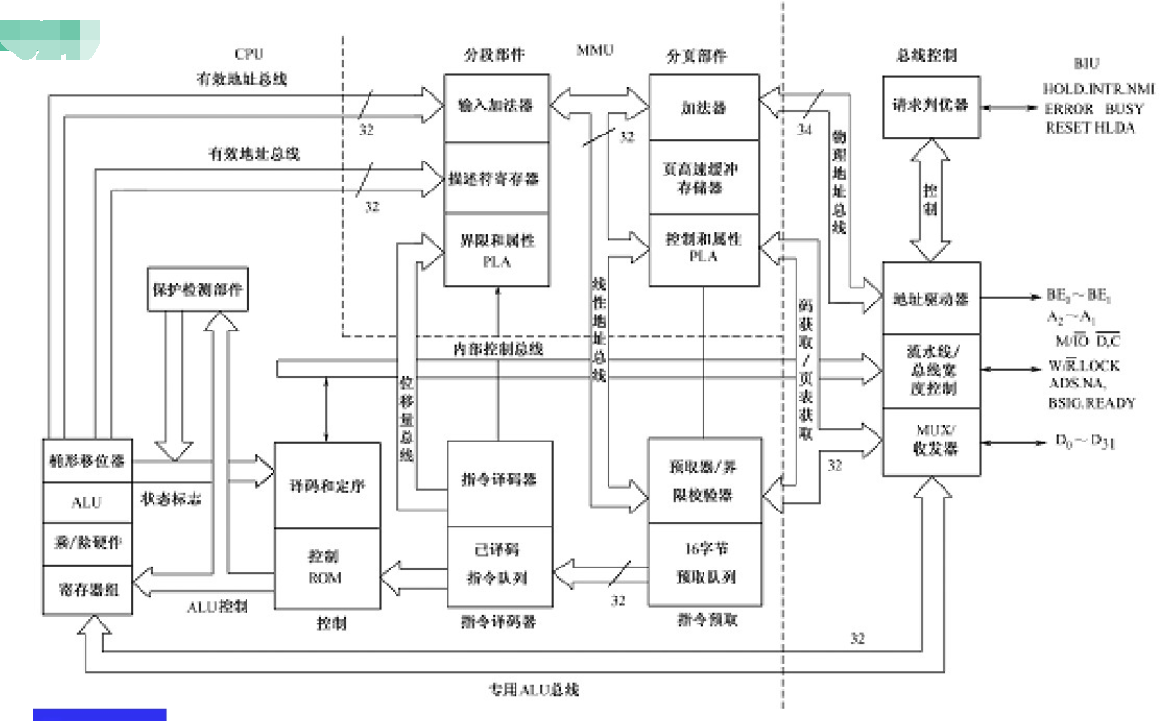
\includegraphics[scale=0.3]{fig/22.png}
\caption{80386结构图}
\label{fig:80386 component}
\end{figure}
总线接口部件  它通过数据总线、地址总线、控制总线来与外部环境联系,包括从存储器中预取指令、读写数据,从I/O端口读写数据,以及其他的控制功能。数据总线和地址总线都是32位的,由于它们是分开的,所以从存储器中存储数据最快也需要两个时钟周期内完成。\\\\
指令预取部件   IPU:它将存放在存储器中的指令经BIU取到16字节长的预取指令队列中,并向指令译码部件输送指令。\\\\
指令译码部件   IDU :从IPU中取出指令进行译码分析,然后将其放入IDU中的译码指令队列中,供执行部件使用。(容纳3条以译码的指令)\\\\
执行部件  EU: 执行部件EU包含算数逻辑单元ALU,8个32位的通用寄存器,一个64位的多位移位加法器,执行数据处理和运算操作\\\\
存储管理部件(MMU)由分段部件和分页机构组成,实现了从逻辑地址到物理地址的转换,既支持段式存储管理、页式存储管理,也支持段页存储管理。它存储器采用段、页式结构,80386首次将分页机制引入到80X86结构,每页大小为4KB。\\\\
分段部件  SU: 按指令要求,分段部件SU将指令中的逻辑地址转换成线性地址。\\\\
分页部件  PU:分页部件PU将分段部件SU产生的线性地址转换成物理地址,每页容量4KB.当系统不使用分页功能时,线性地址就是物理地址。
\subsection{80386的寄存器}
80386微处理器共有7类34个寄存器,通用寄存器组、段寄存器、指令指针和标志寄存器、系统地址寄存器、控制寄存器、调试寄存器、测试寄存器。\\\\
(1)通用寄存器组:共有8个32位寄存器 EAX EBX ECX EDX ESP EBP ESI EDI 它们由8086的16位寄存器扩展而来,它们的低16位与8086使用方法相同。\\\\
(2)段寄存器:共有6个16位的段寄存器CS、DS、SS、ES、FS、GS。与这6个段寄存器对应的有6个64位描述符寄存器,它是80X86处理器提供的一种附加的非编程的寄存器,用来装64的段描述符,每当一个段选择符被装入段寄存器是,相应的段描述符就由内存装入到对应的非编程的CPU寄存器。其中CS、DS、SS、ES与8086的段寄存器完全相同,在实地址方式下,使用方法也与8086相同;在虚地址保护方式下,这些寄存器中的值是“段选择符”,需要查全局描述符表(GDT)或者局部描述符表(LDT)来获得段的基地址,再加上偏移地址才能得到线性地址。 FS和GS是新加的附加数据段寄存器,可以由用户将FS、GS定义为其他数据段。\\\\
(3)指令指针和标志寄存器:指令指针寄存器EIP,由8086的IP寄存器扩展而来。标志寄存器EFLAGS包含一组状态标志、一个控制标志、一组系统标志。
\begin{figure}[htbp]
\centering
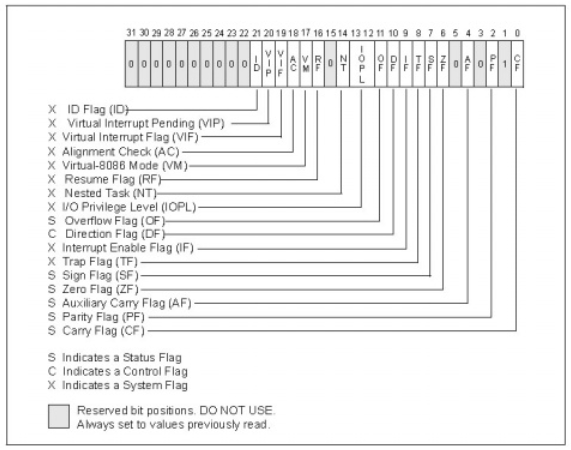
\includegraphics[scale=0.5]{fig/23.png}
\caption{80386 EFLAGS寄存器}
\label{fig:80386 EFLAGS}
\end{figure}
标志寄存器EFLAGS的低12位与8086的标志寄存器FLAGS一样。IOPL位表示特权标志位,定义当前任务的特权层。NT位表示任务嵌套标志位,当NT位为1时表明当前执行的任务嵌套在另外一个任务中,否则NT位为0。NT位控制IRET指令的运行,如果NT=0,用栈中保存的值恢复EFLAGS、CS和EIP执行常规的中断返回; 如果NT=1,中断返回用一任务转换代替上述过程。RF位表示重新启动标志位,与调试寄存器一起用于断点和单步操作,RF位为1时表明下一条指令的调试故障将被忽略,不产生中断异常;RF位位0时表示调试故障被接受并产生中断异常。由于调测失败后强迫程序恢复执行;在每条指令成功执行后,RF自动复位。VM位表示虚拟模式标志位,VM位为1时表明80386工作在保护虚拟地址方式。前4个定义从80286开始,后面的2个定义从80386开始存在。另外的三个标志是Pentium以后的CPU才有的。VIF(Virtual interrupt flag)表示虚拟中断标志。当VIF=1时,可以使用虚拟中断,当VIF=0时不能使用虚拟中断。该标志要和下面的VIP和CR4中的VME配合使用。VIP(Virtual interrupt pending flag)表示虚拟中断挂起标志。当VIP=1时,VIF有效,VIP=0时VIF无效。ID(Identification flag)表示鉴别标志。该标志用来只是Pentium CPU是否支持CPUID的指令。\\\\
(4) 系统地址寄存器和系统段寄存器:系统地址寄存器有全局描述符表寄存器GDTR、中断描述符表寄存器IDTR。系统段寄存器有局部描述符表寄存器LDTR和任务寄存器TR。这些寄存器保存相应的描述符表的地址。\\\\
(5) 控制寄存器:4个32位的控制寄存器CR0,CR1,CR2,CR3,它们保存全局性的机器状态。从Pentium开始,又增加了一个CR4。\\
\begin{figure}[htbp]
\centering
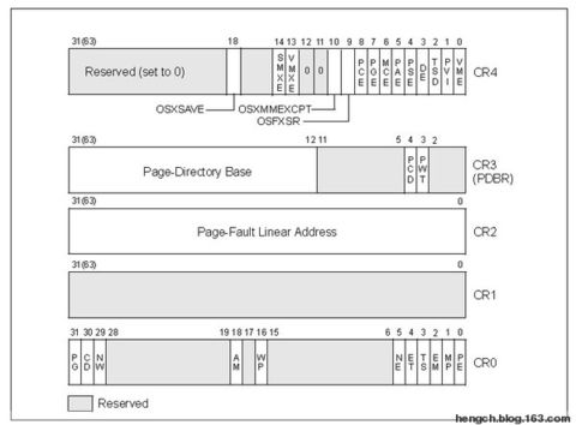
\includegraphics[scale=0.5]{fig/24.png}
\caption{80386 控制寄存器}
\label{fig:80386 CR regeisters}
\end{figure}
(1)CR0的低16位包含了与80286的MSW一致的位定义,保持了和80286的兼容,同时也兼容了从80286开始的两条指令LMSW/SMSW。指令LMSW和SMSW分别用于装入和保存机器状态字信息,可以通过MOV指令对CR0进行读写操作。CR0中各位含义如下:\\
PE(Protection Enable)保护模式允许位,用来启动CPU进入虚地址保护方式。PE=0表示CPU工作在实地址方式;PE=1表示CPU工作在虚地址保护方式。\\
MP(Monitor Coprocessor)监控协处理器,MP=1表示协处理器在工作;MP=0表示协处理器未工作。 \\
EM(Emulation)协处理器仿真,当MP=0,EM=1时,表示正在使用软件仿真协处理器工作。 \\
TS(Task Switched)任务转换,每当进行任务转换时,TS=1;任务转换完毕,TS=0。TS=1时不允许协处理器工作。  \\
ET(Extension Type)处理器扩展类型,反映了所扩展的协处理器的类型,ET=0为80287,ET=1为80387。 \\
PG(Paging)页式管理机制使能,PG=1时页式管理机制工作,否则不工作。\\
NE(Numeric Error)数值异常中断控制,NE=1时,如果运行协处理器指令发生故障,则用异常中断处理,NE=0时,则用外部中断处理。 \\
WP(Write Protect)写保护,当WP=1时,对只读页面进行写操作会产生页故障。\\
AM(Alignment Mask)对齐标志,AM=1时,允许对齐检查,AM=0时不允许,关于对齐,在EFLAGS的AC标志时介绍过,在80486以后的CPU中,CPU进行对齐检查需要满足三个条件,AC=1、AM=1并且当前特权级为3。 \\
NW(Not Write-through)和CD(Cache Disable),这两个标志都是用来控制CPU内部的CACHE的,当NW=0且CD=0时,CACHE使能,其它的组合比较复杂。
前4个定义从80286开始,接着的2个定义从80386开始存在, 后面4个是从80486开始定义的。\\
(2)CR1寄存器用来保留给Intel微处理器将来开发使用;CR2寄存器包含一个32位的线性地址,指向发生最后一次也故障的地址,只有在PG=1时,CR2才有效,当页故障处理程序被激活时,压入页故障处理程序堆栈中的错误码提供页故障的状态信息;\\
(3)CR3寄存器中包含页物理目录表的物理基地址,由于每4KB为一页,80386中的页目录表总在页的整数边界上,CR3的低13位总是为0,只有当CR0中的PG=1时,CR3的页目录基地址才有效。\\\\
(6) 调试寄存器:共8个排错寄存器DR0~DR7。DR0~DR3可以分别设置4个断点的线性地址,DR4~DR5保留未用,DR6是断点状态寄存器,DR7是断点控制寄存器(包括断点类型、断点长度,断点开放/禁止)。\\\\
(7) 测试寄存器:2个32位的测试寄存器TR6和TR7,用于控制转换后援缓冲器中的RAM测试,其中TR6为命令测试寄存器,TR7为测试数据寄存器。
\subsection{80386工作模式}
80386有三种工作模式:实地址模式、保护虚拟地址模式和虚拟8086模式。常用的WINDOWS,LINUX 就是工作在处理器的保护模式底下.为了兼容以前在实模式底下工作的软件,80386支持实模式,但是在实模式底下不能支持多任务处理,所以V86模式应运而生.
\paragraph{实模式} 
80386工作在时模式底下时 A0--------A19的20根地址线是可用的,寻址空间为1MB,这个时候80386和8086,8088的寻址方式是一样的,即段寄存器内容左移4位作为段地址,在加上段内偏移地址就构成了20位的物理地址,每个段的最大长度是64K,所以实模式底下物理地址的最高为是0XFFFFFH,若超除了就会被丢弃.在这种模式底下,80386不支持优先级,所以程序都可执行特权指令,不支持硬件上多任务的切换,是单操作系统.定位中断服务子程序,需要中断向量表,中断向量号乘以4得到中断向量号,再在表中查找中断向量,中断向量有4个字节组成,分别是两个字节的段地址和两个字节的偏移地址,就可得到中断服务程序的入口地址. 这种模式底下可以直接对I/O地址空间,数据段,代码段进行读写.这时的80386和8086非常相似,80386就象是一个快速的8086,只不过80386有32位的数据线和32位的通用寄存器而8086是16位的.准确的说是准16位的系统
\paragraph{保护模式} 
在保护模式底下,逻辑地址由段寄存器和偏移地址组成,不过要得到物理地址可不是实模式底下的方法,首先,段寄存器中存放的不是段基址,而是选择子,系统通过选择子来得到真正的段基地址,然后段基地址和偏移地址相加后得到线性地址,这是通过分段机制实现的,然后再通过分页机制把线性地址转化成物理地址.但是分页机制是可选的.在保护模式底下,32条地址线全部有效,最大寻址空间可达4GB.支持多任务处理,使用一条指令或者一个中断就可以在任务内或任务间切换.提供了0---3共4个特权级,操作系统运行在最高级上即0级,应用程序运行低级上,不但实现资源共享,而且实现数据和代码的安全.不再使用中断向量表来实现中断功能,而是通过各种控制描述符来和特权级检查来完成多任务的实现即中断功能.以前那些I/O操作的指令不能对I/O端口进行读写,通过特权级和I/O许可位来进行安全检查.
\paragraph{V86模式} 
V86模式就是想利用保护模式的优点来运行8086下的程序.它是在保护模式底下工作的,也称虚拟8086模式.v86模式底下寻址和实模式相同,但20位地址不是真实的物理地址,而是线性地址,寻址空间为1MB,为了使多个虚8086任务不使用同一个位置的1MB地址空间,系统使用了分页机制将不同的V8086任务映射到不同的物理空间上去.每个V86任务认为自己在0-1MB的空间上运行.这样8086下的程序可以在80386的V86模式底下运行,但是它的一部分指令是是受到保护的,如果执行将发生异常,V86模式受到了V86监控程序的控制,v86监控程序和硬件组成了"8086虚拟机"。V86监控程序控制外部界面,中断,I/O,硬件提供最底端的1MB虚拟存储.,在80386中每个V86模式是相对的,这样就充分发挥了处理器的能力
%https://www.cnblogs.com/yilang/p/11330767.html
\subsection{80386的描述符}
\begin{figure}[htbp]
\centering
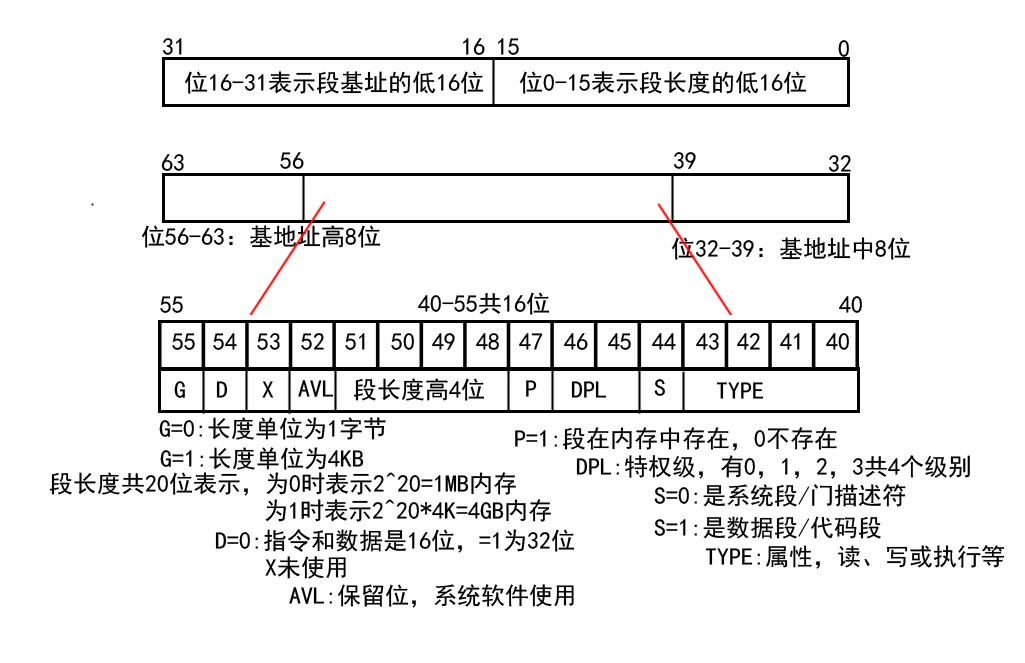
\includegraphics[scale=0.4]{fig/25.jpeg}
\caption{80386 描述符结构}
\label{fig:80386 Segment Descriptor}
\end{figure}
对比80286的描述符结构,可以看出,前48bit基本一致(A bit包含在Type中了)。从49到64的16bit,在80286中是保留的bit,在80386中扩展,其中4bit用于扩充段长,8bit用于扩充段的基地址。TYPE段的详细解释:\\
位0:A(accessed)位,表明描述符是否已被访问;把选择子装入段寄存器时,该位被标记为1;\\
位3:E(EXECUTABLE?)位,0说明所描述段为数据段;1为可执行段(代码段);\\
当为数据段时, 位1为W位,说明该数据段是否可写(0只读,1可写),位2为ED位,说明该段的扩展方向(0向高位扩展,1向低位扩展);\\
当为可执行段时, 位1为R位,说明该执行段是否可读(0只执行,1可读);位2为C位,0说明该段不是一致码段(普通代码段),1为一致码段 。
\subsection{一致和非一致代码段}
一致代码段:简单理解就是操作系统拿出来被共享的代码段,可以被低特权级的用户程序直接调用访问的代码段,这些代码段,通常是不去访问受保护的资源和某些类型异常处理。一致代码段访问限制:\\
特权级高的程序不允许访问特权级第的数据:即内核态不允许调用用户态的数据。\\
特权级低的程序可以访问到特权级高的程序,但是特权级不会改变,即不会从用户态切换到内核态。\\\\
非一致代码段:为了避免低特权级的访问而被操作系统保护起来的系统代码。非一致代码段访问限制:\\
只允许同特权级访问。\\
绝对禁止不同特权级直接访问:内核态不去用户态,用户态也不使用内核态。\\
通常低特权级代码必须通过门调用来实现对高特权级代码段的访问和调用。
\part{IO端口}
\section{IO端口地址范围}
X86将外设的寄存器看成一个独立的地址空间,对外设寄存器的读/写设置专用指令,如IN和OUT指令。这种就是所谓的“I/O端口”方式,即独立编址。
\begin{list}{•}{•}
\item 端口地址范围  分配说明
\item 0x000-0x01f 8237A DMA控制器1
\item 0x020-0x03f 8259A 可编程中断控制器1
\item 0x040-0x05f 8253/8254|A 定时计数器
\item 0x060-0x06f 8042键盘控制器
\item 0x070-0x07f 访问CMOS RAM/实时时钟RTC(Real Time Clock)端口
\item 0x080-0x09f DMA页面寄存器访问端口
\item 0x0a0-0x0bf 8259 可编程中断控制器2
\item 0x0c0-0x0df 8237A DMA控制器2
\item 0x0f0-0x0ff 协处理器访问端口
\item 0x170-0x177 IDE硬盘控制器1
\item 0x1f0-0x1f7 IDE硬盘控制器2
\item 0x278-ox27f 并行打印机端口2
\item 0x2f8-0x2ff 串行控制器2
\item 0x378-0x38f 并行打印机端口1 
\item 0x3b0-0x3bf 单色MDA显示控制器
\item 0x3c0-0x3cf 彩色CGA显示控制器
\item 0x3d0-0x3df 彩色EGA/VGA显示控制器
\item 0x3f0-0x3f7 软盘控制器
\item 0x3f8-0x3ff 串行控制器1
\end{list}{•}{•}
具体的,020-02F为8259A Master Programmable Interrupt Controller:
\begin{list}{•}{•}
\item 020 8259 Command port (see 8259)
\item 021 8259 Interrupt mask register (see 8259)
\end{list}{•}{•}
040-05F为8253 or 8254 Programmable Interval Timer:
\begin{list}{•}{•}
\item 040 8253 channel 0, counter divisor
\item 041 8253 channel 1, RAM refresh counter
\item 042 8253 channel 2, Cassette and speaker functions
\item 043 8253 mode control (see 8253)
\item 044 8254 PS/2 extended timer
\item 047 8254 Channel 3 control byte
\end{list}{•}{•}
060-06f为8042 Keyboard Controller (AT,PS2):
\begin{list}{•}{•}
\item 060 8042 Keyboard input/output buffer register
\item 061 8042 system control port (for compatability with 8255)
\item 064 8042 Keyboard command/status register
\end{list}{•}{•}
\part{中断控制器}
可编程中断控制器(PIC - Programmable Interrupt Controller)是微机系统中管理设备中断请求的管理者。当PIC向处理器的INT引脚发出一个中断信号时,处理器会立刻停下当时所做的事情并询问PIC需要执行哪个中断服务请求。PIC则通过向数据总线发出与中断请求对应的中断号来告知处理器要执行哪个中断服务过程。处理器则根据读取的中断号通过查询中断向量表(在32位保护模式下是中断描述符表)取得相关设备的中断向量(即中断服务程序的地址)并开始执行中断服务程序。当中断服务程序执行结束,处理器就继续执行被中断信号打断的程序。
\section{8259A芯片}
早期的IBM PC/XT只有一个8259A,一个8259A芯片可以管理8个中断源。这样就只能处理8种IRQ。但很快就发现这根本不能满足需求,所以到了IBM PC/AT,又以级连的方式增加了一个8259A,这样就可以多处理7种IRQ。原来的8259A被称作Master PIC,新增的被称作Slave PIC。但由于CPU只有1根中断线,Slave PIC不得不级连在Master PIC上,占用了IRQ2,设计者从Slave PIC的IRQ中挑出IRQ9,要求软件设计者将原来的IRQ2重定向到IRQ9上,也就是说IRQ9的中断服务程序需要去调用原来IRQ2的中断服务程序。这样,将原来接在IRQ2上的设备现在接在IRQ9上,在软件上只需要增加IRQ9的中断服务程序,由它调用IRQ2的中断服务程序,就可以和原有系统保持兼容。而在当时,增加的IRQ9中断服务程序是由PC开发商开发的BIOS提供的,不需要用户进行另外设置,所以就从根本上保证了兼容。
\begin{figure}[htbp]
\centering
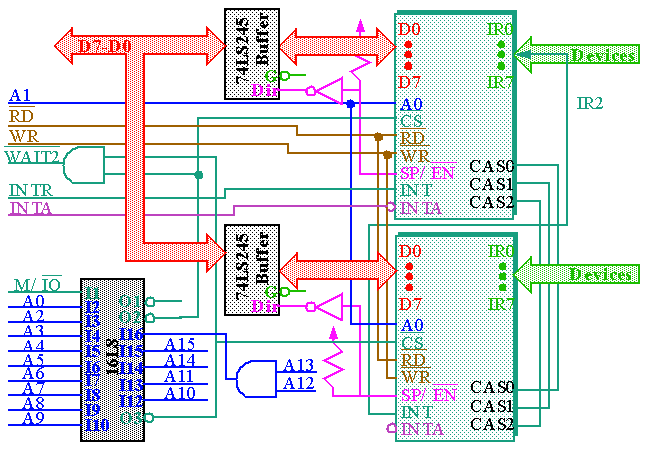
\includegraphics[scale=0.4]{fig/8.png}
\caption{8259及其级联}
\label{fig:8259 and its cascading}
\end{figure}
\begin{list}{•}{•}
\item WR: Connects to a write strobe signal (one of 8 for the Pentium).
\item RD: Connects to the IORC signal.
\item INT: Connects to the INTR pin on the microprocessor.
\item INTA: Connects to the INTA pin on the microprocessor.
\item A0: Selects different command words in the 8259A.
\item CS: Chip select - enables the 8259A for programming and control.
\item SP/EN: Slave Program (1 for master, 0 for slave)/Enable Buffer (controls the data bus transievers when in buffered mode).
\item CAS2-CAS0: Used as outputs from the master to the slaves in cascaded systems.
\end{list}
A0线用于选择操作的寄存器。在PC/AT微机系统中,当A0=0时芯片的端口地址是0x20(主芯片)和0xA0(从芯片);当 A0=1时端口就是0x21(主芯片)和0xA1(从芯片)。 
\section{8259A的状态}
在总线控制器控制下,8259A芯片可以处于编程状态和操作状态。编程状态是CPU使用IN或OUT指令对8259A芯片进行初始化编程的状态。一旦完成了初始化编程,芯片即进入操作状态,此时芯片即可随时响应外部设备提出的中断请求(IRQ0 -IRQ15),同时系统还可以使用操作命令字随时修改其中断处理方式。
\section{8259A的初始化}
在8259A可以正常工作之前,必须首先设置初始化命令字 ICW (Initialization Command Words)寄存器组的内容。
%http://ece-research.unm.edu/jimp/310/slides/8086_interrupts.html
\begin{lstlisting}[breaklines]
There are 4 ICWs.
    At power-up, ICW1, ICW2 and ICW4 must be sent.
    If ICW1 indicates cascade mode, then ICW3 must also be sent.
\end{lstlisting}
\begin{figure}[htbp]
\centering
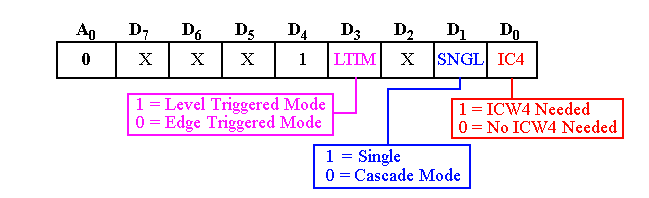
\includegraphics[scale=0.4]{fig/2.png}
\caption{ICW1}
\label{fig:8259 ICW1}
\end{figure}
在此,ICW1 被设置为 0x11。表示中断请求是边沿触发、多片 8259A 级联并且需要发送 ICW4。在对主芯片设置了ICW1之后,0x00eb,0x00eb 和jmp short \$+2 差不多,都是因为 I/O 的端口延时, 延时几微秒给端口一个反应时间。\\\\
接下来对 ICW2 进行设置,8259A主芯片的端口地址是0x21,从芯片的端口地址是0xA1。ICW2的 T7~T3 是中断号的高5位,与 8259A 芯片自动设置的低3位(8259A 按 IR0~IR7 三位编码值自动填入)组成一个8位的中断号。
\begin{figure}[htbp]
\centering
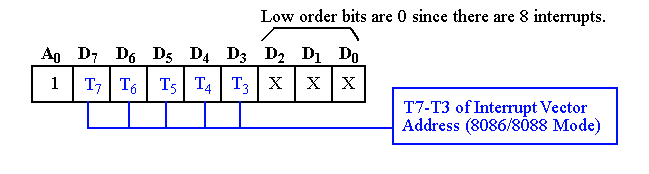
\includegraphics[scale=0.5]{fig/3.png}
\caption{ICW2}
\label{fig:8259 ICW2}
\end{figure}
这里把主片的 ICW2 设置为 0x20,表示主片中断请求0~7级对应的中断号是 0x20~0x27;把从片的 ICW2 设置成 0x28,表示从片中断请求8~15级对应的中断号是 0x28~0x2f。 \\\\
接下来是ICW3:
\begin{figure}[htbp]
\centering
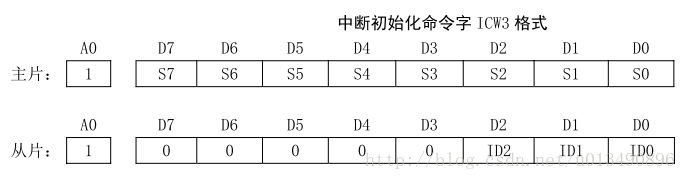
\includegraphics[scale=0.6]{fig/4.png}
\caption{ICW3}
\label{fig:8259 ICW3}
\end{figure}
这里把8259A主片的 ICW3 设置为 0x04,即 S2=1,其余各位为0。表示主芯片的 IR2 引脚连接一个从芯片。从芯片的 ICW3 被设置为 0x02,即其标识号为2。表示此从片连接到主片的IR2引脚。 因此,中断优先级的排列次序为:0级最高,1级次之,接下来是从片上的 8~15 级,最后是主片的 3~7 级。 \\\\
接下来是ICW4:
\begin{figure}[htbp]
\centering
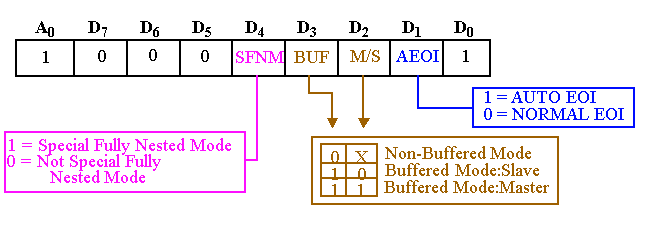
\includegraphics[scale=0.5]{fig/5.png}
\caption{ICW4}
\label{fig:8259 ICW4}
\end{figure}
这里送往8259A主芯片和从芯片的 ICW4 命令字的值均为 0x01。表示 8259A 芯片被设置成普通全嵌套、非缓冲、非自动结束中断方式,并且用于 8086 及其兼容系统。
\section{8259A的工作状态}
在对 8259A 设置了初始化命令字后,芯片就已准备好接收设备的中断请求信号了。在 8259A 工作期间,我们也可以利用操作命令字 OCW1~OCW3 来监测 8259A 的工作状况,或者随时改变初始化时设定的 8259A 的工作方式。操作命令字OCW1~OCW3的设置没有规定其先后顺序,使用时可根据需要灵活选择不同的操作命令字写入到8259A中。\\\\
\begin{figure}[htbp]
\centering
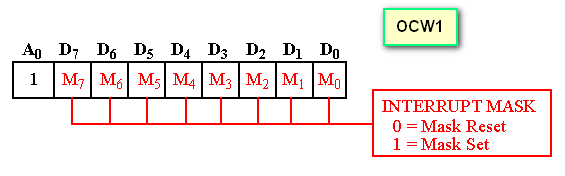
\includegraphics[scale=0.6]{fig/6.png}
\caption{OCW1}
\label{fig:8259 OCW1}
\end{figure}
这里在设置好相关的设备驱动程序后就会利用该操作命令字屏蔽中断请求。
\part{键盘控制器}
\section{8042/8048芯片}
和键盘相关的最重要的硬件是两个芯片,一个是 intel 8042 芯片,位于主板上,CPU 通过 IO 端口直接和这个芯片通信;另一个是 intel 8048 芯片或者其兼容芯片,位于键盘中,这个芯片主要作用是从键盘的硬件中得到被按的键所产生的扫描码,与 8042 通信,控制键盘本身。所以对于驱动来说,直接发生联系的只有 8042。
\section{8042的寄存器}
8042 有 4 个 8 bits 的寄存器,他们是 Status Register(状态寄存器),Output Buffer(输出缓冲器),Input Buffer(输入缓冲器),Control Register(控制寄存器)。使用两个 IO 端口,60h (数据端口)和 64h(命令端口)。代码中首先在64h端口上写入D1h,表示准备写Output端口。随后通过60h端口写入的字节,会被放置在Output Port中;然后在60h端口上写入了0xDF。
\section{端口61h}
通过0x61端口可读入键盘状态,设置禁止单板工作,然后再恢复,起到复位键盘的作用。61H早期用于8255B口,bit 7用于应答键盘(仅早期pc机),bit 0~1用于开关8253/4输出到SPEAKER,其他的位不要去动。
\section{8042的读写命令}
驱动对键盘控制器发送命令是通过写端口64h实现的,共有12条命令:
\begin{list}{•}{•}
\item 20h 准备读取8042芯片的Command Byte;其行为是将当前8042 Command Byte的内容放置于Output Register中,下一个从60H端口的读操作将会将其读取出来。
\item 60h 准备写入8042芯片的Command Byte;下一个通过60h写入的字节将会被放入Command Byte。
\item A4h 测试一下键盘密码是否被设置;测试结果放置在Output Register,然后可以通过60h读取出来。测试结果可以有两种值:FAh=密码被设置;F1h=没有密码。
\item A5h 设置键盘密码。其结果被按照顺序通过60h端口一个一个被放置在Input Register中。密码的最后是一个空字节(内容为0)。
\item A6h 让密码生效。在发布这个命令之前,必须首先使用A5h命令设置密码。
\item AAh 自检。诊断结果放置在Output Register中,可以通过60h读取。55h=OK。
\item ADh 禁止键盘接口。Command Byte的bit-4被设置。当此命令被发布后,Keyboard将被禁止发送数据到Output Register。
\item AEh 打开键盘接口。Command Byte的bit-4被清除。当此命令被发布后,Keyboard将被允许发送数据到Output Register。
\item C0h 准备读取Input Port。Input Port的内容被放置于Output Register中,随后可以通过60h端口读取。
\item D0h 准备读取Outport端口。结果被放在Output Register中,随后通过60h端口读取出来。
\item D1h 准备写Output端口。随后通过60h端口写入的字节,会被放置在Output Port中。
\item D2h 准备写数据到Output Register中。随后通过60h写入到Input Register的字节会被放入到Output Register中,此功能被用来模拟来自于Keyboard发送的数据。如果中断被允许,则会触发一个中断。

\part{可编程计数器/定时器}
\section{8253芯片}
intel8253是NMOS工艺制成的可编程计数器/定时器,有几种芯片型号,外形引脚及功能都是兼容的,只是工作的最高计数速率有所差异,例如8253(2.6MHz),8253-5(5MHz)。8253内部有三个完全独立的计数器,分别称为计数器0、计数器1和计数器2,他们的机构完全相同。每个计数器通过三个引脚和外部联系,一个为时钟输入端CLK,一个为门控信号输入端GATE,另一个为输出端OUT。

\begin{figure}[htbp]
\centering
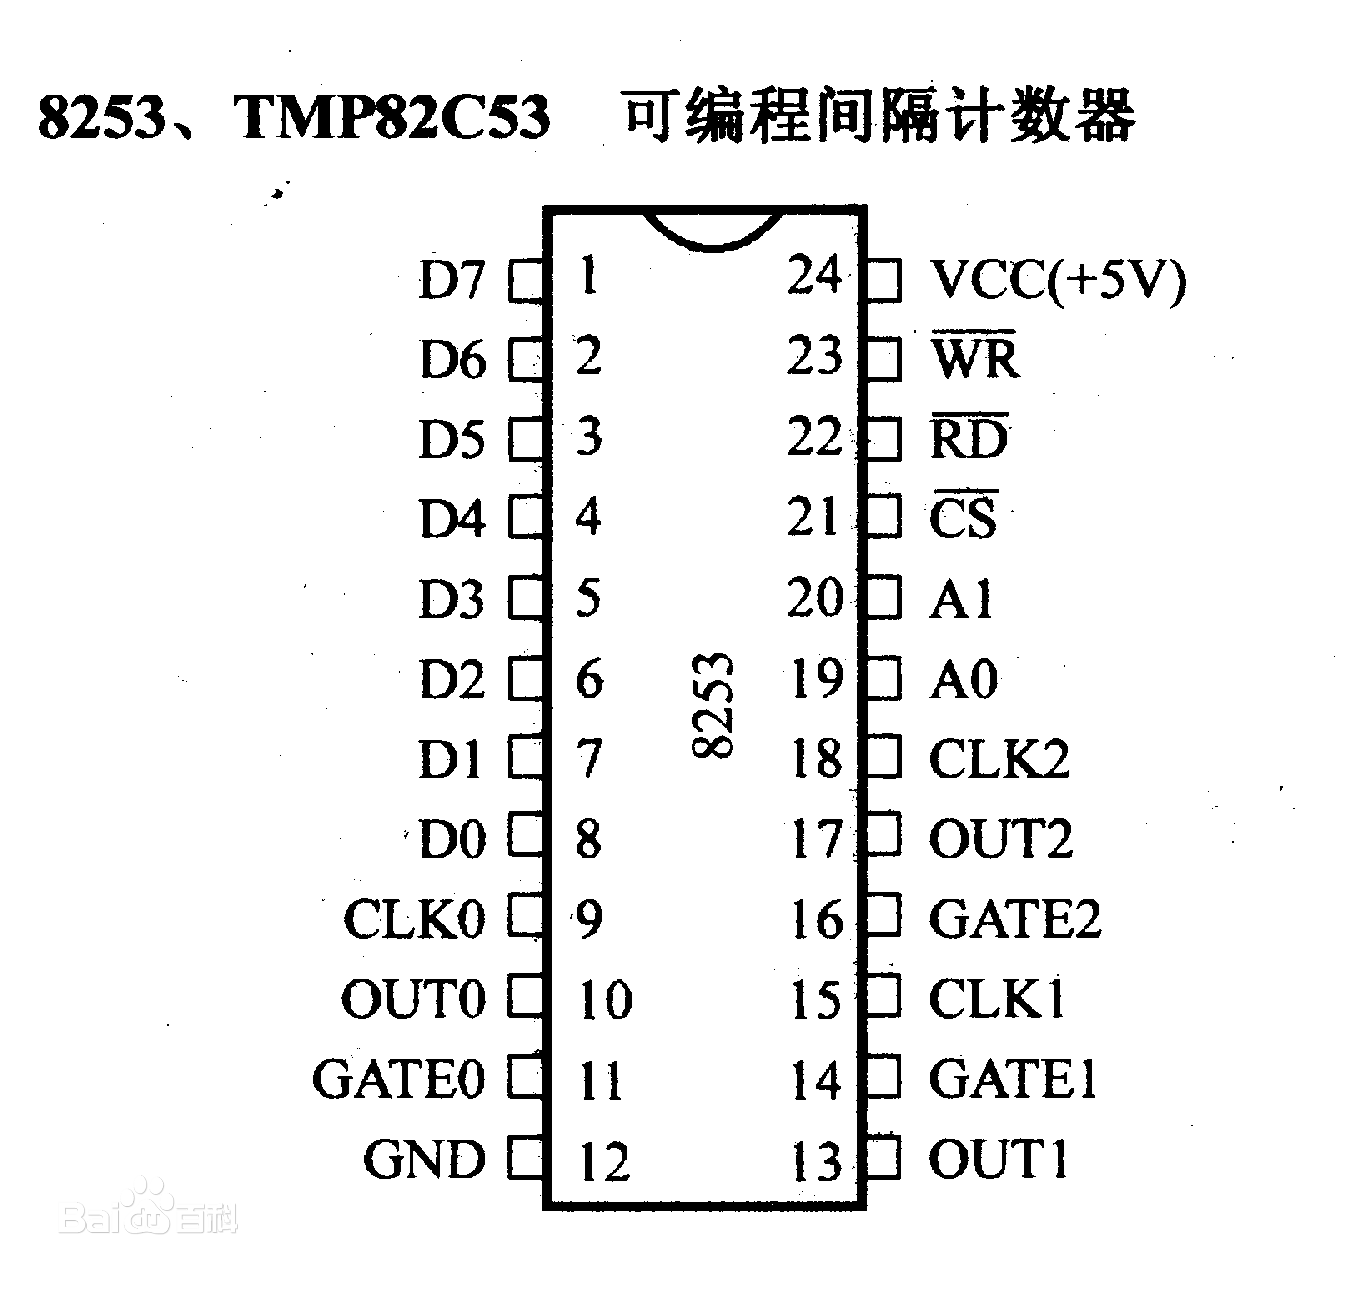
\includegraphics[scale=0.15]{fig/26.png}
\caption{8253芯片引脚定义}
\label{fig:Intel 8253 Chip outlook}
\end{figure}

\begin{enumerate}
\item D0~D7, 数据总线缓冲器与系统总线连接,8位双向,与CPU交换信息的通道。这是8253与CPU之间的数据接口,它由8位双向三态缓冲存储器构成,是CPU与8253之间交换信息的必经之路。
\item A0A1,端口选择信号,由CPU输入。8253内部有3个独立的通道,加上控制字寄存器,构成8253芯片的4个端口,CPU可对3个通道进行读/写操作3对控制字寄存器进行写操作。
\item CS\#,片选信号,由CPU输入,低电平有效,通常由端口地址的高位地址译码形成。
\item RD\#、WR\#,读/写控制命令,由CPU输入, 低电平有效。RD\#效时,CPU读取由A1A0所选定的通道内计数器的内容。WR\#有效时,CPU将计数值写入各个通道的计数器中, 或者是将方式控制字写入控制字寄存器中。
\end{enumerate}

\section{8253的通道和端口}
8253内部有3个独立的通道,加上控制字寄存器,构成8253芯片的4个端口。
\begin{figure}[htbp]
\centering
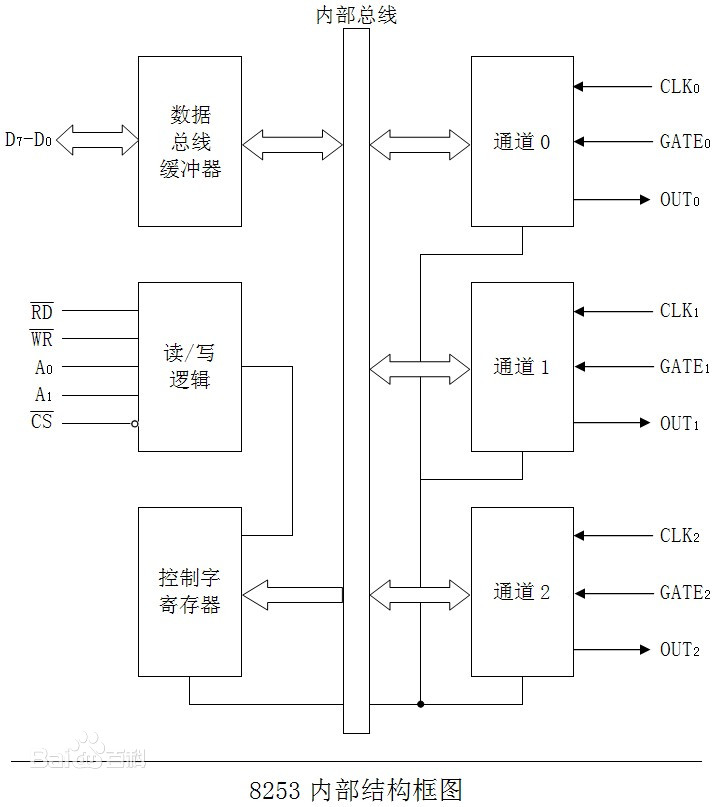
\includegraphics[scale=0.4]{fig/27.jpeg}
\caption{8253内部结构框图}
\label{fig:Intel 8253 inner structure}
\end{figure}

每个计数器内部有一个8位的控制寄存器,还有一个16位的计数初值寄存器CR、一个计数执行部件CE和一个输出锁存器OL。每个计数器的输入和输出都决定于设置在控制寄存器中的控制字,互相之间工作完全独立。
\\\\
计数器可进行二进制或十进制(BCD码)计数。采用二进制计数时, 写入的初值范围为0000H~0FFFFH,最大计数值是0000H,代表65536。 采用BCD码计数时,写入的初值范围为0000~9999,最大计数值是0000,代表10000。与此计数器相对应,每个通道内设有一个16位计数值锁存器。必要时可用来锁存计数值。(特别说明:8253计数器的值先减1再判断是否为0,为0就中断了,所以最大初始值为0,这样减1以后,不为0,所以为最大的,取决于CF标志位)。
\\\\
8253中各通道可有6种可供选择的工作方式, 以完成定时、计数或脉冲发生器等多种功能。当用作计数器时,应将要求计数的次数预置到该通道的计数器中、被计数的事件应以脉冲方式从CLK端输入, 每输入一个计数脉冲,计数器内容减“1”,待计数值计到“0”。 OUT端将有输出,表示计数次数到;当用作定时器时。 由CLK输入一定频率的时钟脉冲。根据要求定时的时间长短确定所需的计数值,并预置到计数器中。每输入一个时钟脉冲,计数器内容减“1”, 待计数值计到“0”,OUT将有输出,表示定时时间到。允许从CLK输入的时钟频在1~2MHz范围内。8253的各种工作方式如下:
\begin{enumerate}
\item 方式0:计数结束则中断。当CPU利用输出指令向该通道写入计数值WR\#有效时,OUTi保持低电平,然后计数器开始减“1”计数, 直到计数值为“0”,此刻OUTi将输出由低电平向高电平跳变,可用它向CPU发出中断请求,OUTi端输出的高电平一直维持到下次再写入计数值为止
\item 方式1:单脉冲发生器。CPU装入计数值n后OUTi输出高电平,不管此时的GATE输入是高电平还是低电平,都不开始减“1”计数,必须等到GATE由低电平向高电平跳变形成一个上升沿后,计数过程才会开始。与此同时,OUTi输出由高电平向低电平跳变,形成了输出单脉冲的前沿,待计数值计到“0”, OUTi输出由低电平向高电平跳变,形成输出单脉冲的后沿, 因此,由方式l所能输出单脉冲的宽度为CLKi周期的n倍。
\item 方式2:速率波发生器。装入计数值n后如果GATE为高电平,则立即开始计数,OUTi保持为高电平不变; 待计数值减到“1”和“0”之间, OUTi将输出宽度为一个CLKi周期的负脉冲,计数值为“0”时,自动重新装入计数初值n,实现循环计数,OUTi将输出一定频率的负脉冲序列, 其脉冲宽度固定为一个CLKi周期, 重复周期为CLKi周期的n倍。
\item 方式3:方波发生器。如果当GATE为高电平,则立即开始减“1”计数,OUTi保持为高电平,若n为偶数,则当计数值减到n/2时,OUTi跳变为低电平,一直保持到计数值为“0”,系统才自动重新置入计数值n,实现循环计数。这时OUTi端输出的周期为n×CLKi周期,占空比为1:1的方波序列; 若n为奇数, 则OUTi端输出周期为n×CLKi周期,占空比为((n+1)/2)/((n-1)/2)的近似方波序列。
\item 方式4:软件触发方式计数。装入计数值n后, 如果GATE为高电平,则立即开始减“1”计数,直到计数值减到“0”为止,OUTi输出宽度为一个CLKi周期的负脉冲。由软件装入的计数值只有一次有效,如果要继续操作, 必须重新置入计数初值n。
\item 方式5:硬件触发方式计数。硬件触发信号由GATE端引入。 因此,开始时GATE应输入为0, 装入计数初值n后,减“1”计数并不工作,一定要等到硬件触发信号由GATE端引入一个正阶跃信号,减“1”计数才会开始,待计数值计到“0”, OUTi将输出负脉冲,其宽度固定为一个CLKi周期,表示定时时间到或计数次数到。
\end{enumerate}

\section{8253的控制寄存器}
8253的初始化编程就是对其工作方式的确定。具体实现就是在8253上电后,由CPU向8253的控制寄存器写入一个控制字,就可以规定8253的工作方式、计数值的长度以及计数所用的数制等,另外根据要求将计数值写入8253的相应通道。8253的一个方式控制字只决定一个技术通道的工作模式。

\begin{figure}[htbp]
\centering
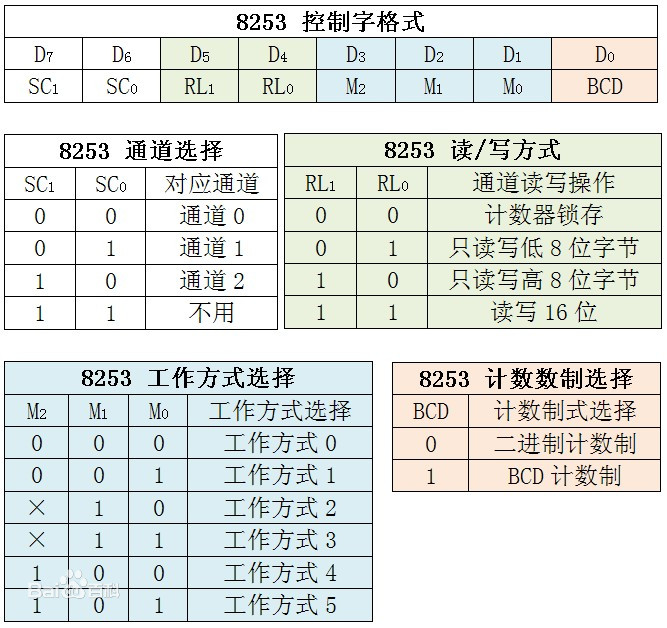
\includegraphics[scale=0.5]{fig/28.jpeg}
\caption{8253控制器格式}
\label{fig:Intel 8253 control word format}
\end{figure}
例如,若设置通道0以读写16位的方式、工作在方式3、计数器值采用二进制,则控制字应为00110110。PC默认分配给8253三个计数器的端口地址分别为40H~42H,控制字寄存器的端口址为43H。则首先向控制器寄存器端口写入控制字,把计数器通道0设置成每隔10毫秒向中断控制器发送一个中断请求信号;然后向计数器通道0写入计数器初始值。
\begin{lstlisting}   
	movb $0x36, %al #00110110
	movl $0x43, %edx
	outb %al, %dx
	movl $11930, %eax # timer frequency 100 HZ 
	movl $0x40, %edx
	outb %al, %dx
	movb %ah, %al
	outb %al, %dx
\end{lstlisting}

\end{list}{•}{•}
\part{Vim设置}
\section{给Vim增加tag功能}
\subsection{安装ctags}
sudo apt-get install ctags \\
实际安装的是:exuberant-ctags
\subsection{建立文件索引}
在想要建立索引文件的文件夹目录下执行\\
sudo ctags -R *
\subsection{通过tag跳转}
运行vim的时候,必须在"tags"文件所在的目录下运行。否则,运行vim的时候还要用":set tags="命令设定"tags"文件的路径,这样vim才能找到"tags"文件。\\\\
把光标移到变量名或函数名上,然后按下"Ctrl-]"。用"Ctrl-o"退回原来的地方。
\subsection{安装taglist}
taglist的下载路径:\\
\url {https://www.vim.org/scripts/script.php?script_id=273} \\\\
解压文件,复制到vim的目录下\\
sudo cp taglist.vim /usr/share/vim/vim81/plugin/ \\
sudo cp taglist.txt /usr/share/vim/vim81/doc/
\subsection{打开和关闭taglist窗口}
启动vim,用“:TlistToggle”来打开和关闭taglist窗口;
\end{CJK}
\end{document}